% SPDX-License-Identifier: CC-BY-SA-4.0
% Author: Matthieu Perrin

\title[Programmation concurrente en multi-threads]{Programmation concurrente en multi-threads}

\author[Matthieu Perrin]{
  \structure{Matthieu \textsc{Perrin}}\\[2mm]
  Nantes Université\\
  Laboratoire des Sciences du Numérique de Nantes \\
  UMR CNRS 6004\\
  Bureau 410, bâtiment 34 \\
  \url{matthieu.perrin@univ-nantes.fr}\\
}

\date{
  Nantes Université\\
  Master en Informatique, première année\\
  Parcours ALMA\\
  2025-2026
}

\begin{document}

\begin{frame}[plain,noframenumbering]
  \titlepage
  \on[text, bottom=-5mm]{\scriptsize
    \begin{description}
    \item[Licence :] \href{https://creativecommons.org/licenses/by-sa/4.0/}{CC BY-SA 4.0} (\ccbysa{}) — Matthieu Perrin
    \item[Code source :]\vspace{-.5mm}  \url{https://github.com/ProgrammationMultiThread/}
    \end{description}
  }
\end{frame}

\part{Introduction}

\begin{frame}{Vue générale}

  \begin{shadequote}{Ancienne documentation de Java}
    If you can get away with it, avoid using threads. Threads can be difficult to use, and they make programs harder to debug.
  \end{shadequote}
  
  \begin{alertblock}{But du cours}
    \begin{itemize}
    \item Comprendre les problèmes inhérents aux systèmes répartis
    \item Apprendre à raisonner sur la concurrence
    \item Déjouer les fausses intuitions
    \item Être en mesure de lire les documentations officielles
    \item Mettre en œuvre les solutions les plus simples
    \end{itemize}
  \end{alertblock}
  \begin{alertblock}{Langages}
    \begin{itemize}
    \item Principalement Java
    \item Généralisations bienvenues
    \end{itemize}
  \end{alertblock}
\end{frame}

\begin{frame}{Bibliographie}
  %\vfill
  \begin{block}{Sites Web}
    \begin{itemize}
    \item \href{http://docs.oracle.com/javase/tutorial/essential/concurrency/index.html}{docs.oracle.com/javase/tutorial/essential/concurrency/index.html}
    \item \href{https://jenkov.com/tutorials/java-concurrency/index.html}{https://jenkov.com/tutorials/java-concurrency/index.html}
    \end{itemize}
  \end{block}

  \vfill

  \begin{block}{Ouvrages}
    \begin{itemize}
    \item \textit{The Art of Multiprocessor Programming}\\ Maurice Herlihy \& Nir Shavit (Morgan Kaufmann 2008)
    \item \textit{Concurrent Programming -- Algorithms, Principles, and Foundations}\\ Michel Raynal (Springer 2013)
    \item \textit{Concurrent Programming in Java: Design Principles and Patterns}\\ Doug Lea (Addison-Wesley 1996)
    \end{itemize}
  \end{block}
  
  \vfill
  \vfill
  
  \begin{citing}
  \item Les articles et ouvrages sont sur Madoc.
    \jitem Les exemples de code du cours et les TP sont dans un projet sur Madoc.
  \end{citing}
\end{frame}


\section{Du parallélisme à la concurrence}
\subsection{Motivations}
\mode*


%%%%%%%%%%%%%%%%%%%%%%%%%%%%%%%%%%%%%%%%%%%%%%%%%%%%%%%%%%%%%%%%%%%%%%%%% 


\begin{frame}
  \frametitle{Fin de la loi de Moore ?}
  \begin{center}
    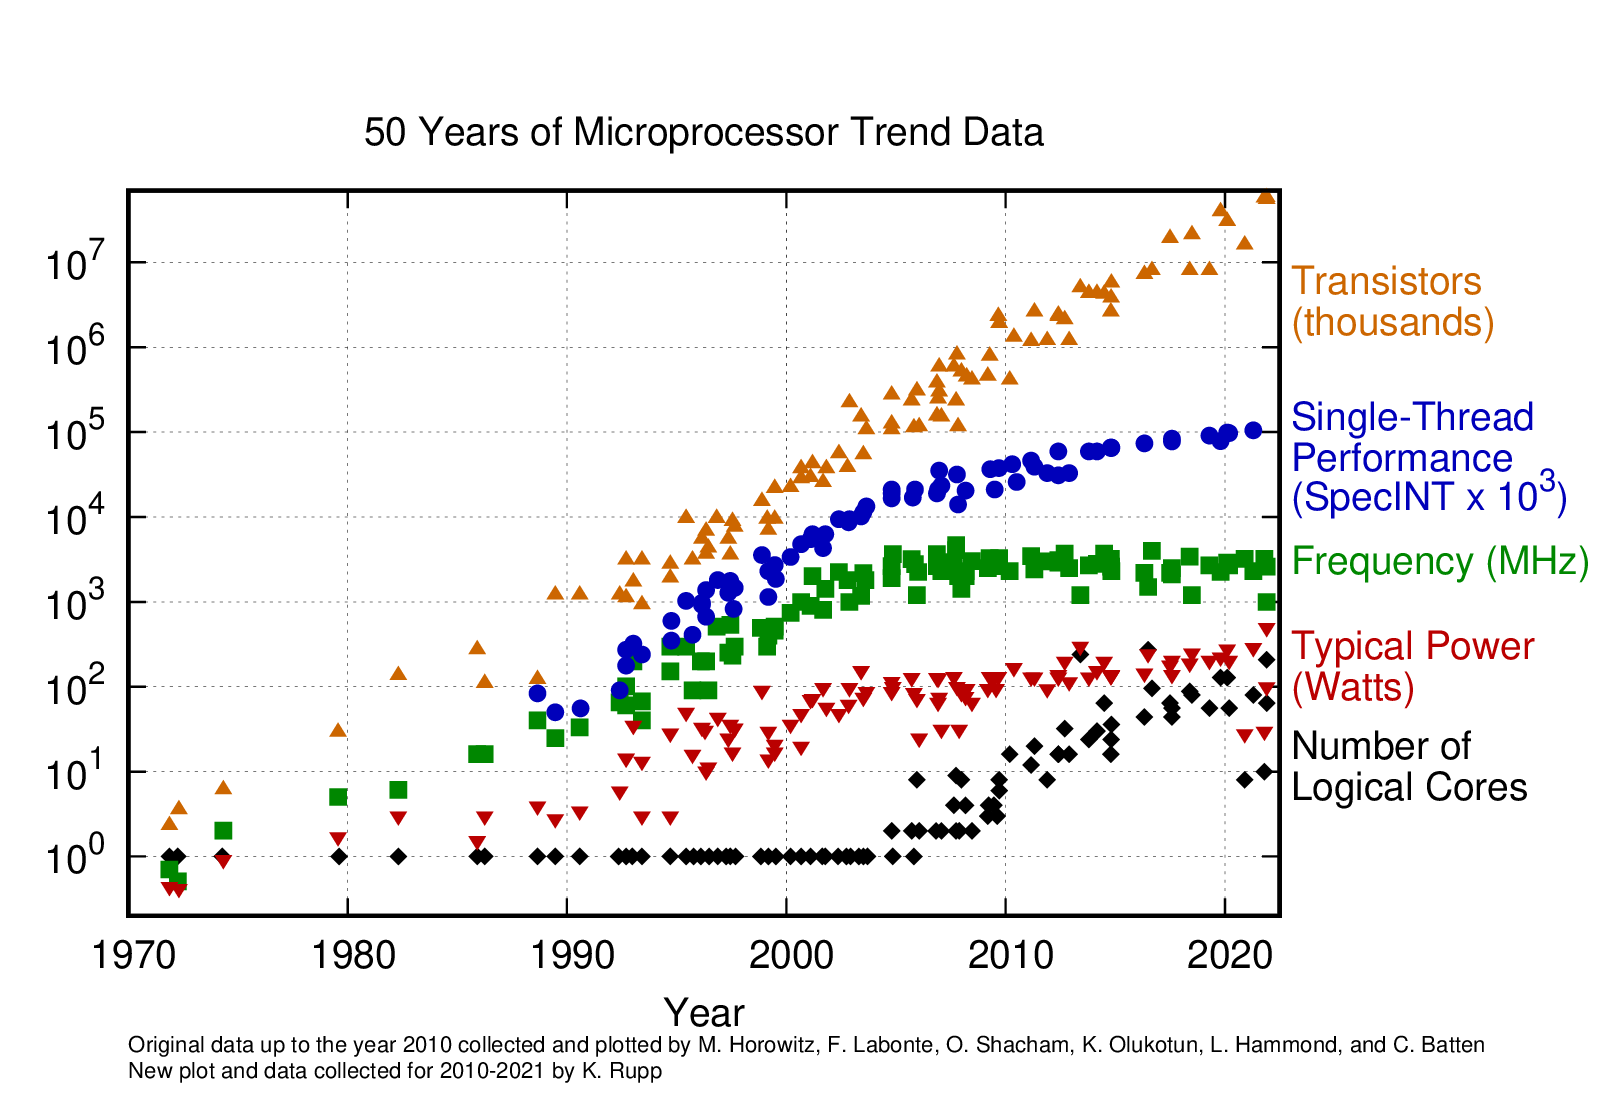
\includegraphics[width=.7\textwidth]{50-years-processor-trend.png}
    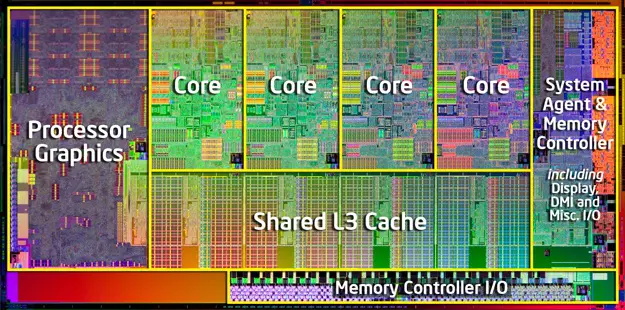
\includegraphics[width=.4\textwidth]{multic.png}
  \end{center}
\end{frame}


\begin{frame}{Buts de la programmation multi-c\oe urs}
   \begin{tikzpicture}[remember picture,overlay]
   \draw (5.5,2.2) node{\begin{minipage}{\textwidth}
      \begin{exampleblock}{Calculs coûteux}
         \begin{itemize}
         \item En temps de processeur (simulations scientifiques, \dots)
         \item<2-> En entrées/sorties (recherche dans les fichiers, \dots)
         \end{itemize}
      \end{exampleblock}
      \end{minipage}
   };

   \draw<1> (5.5,-1) node{
      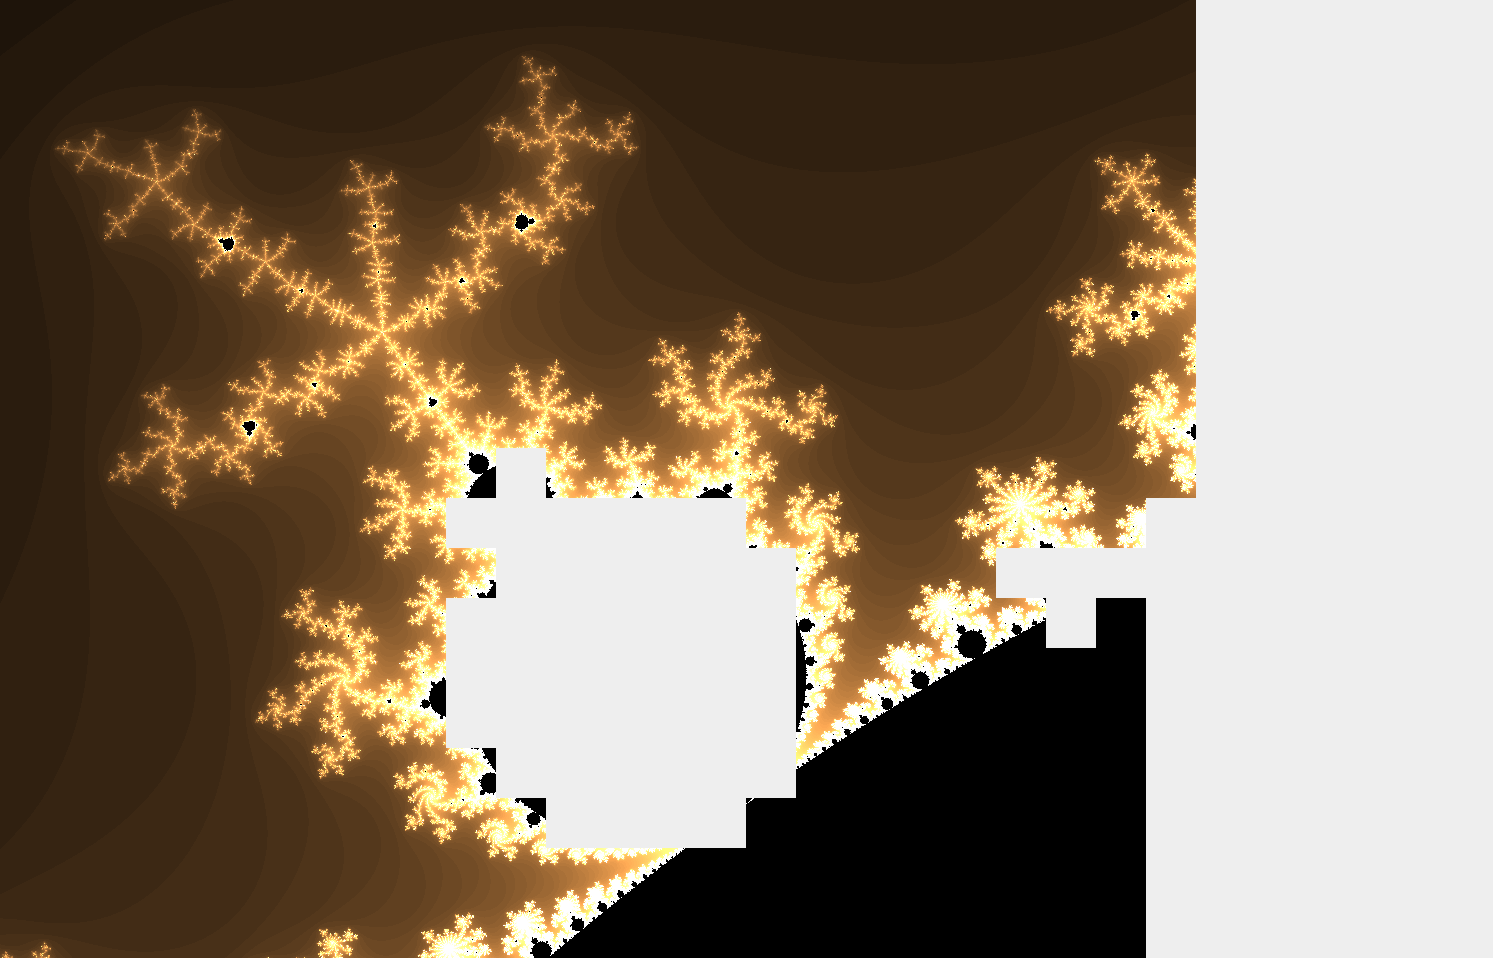
\includegraphics[height=.4\textwidth]{distanciel.png}
   };

   \draw<2> (5.5,-1) node{
        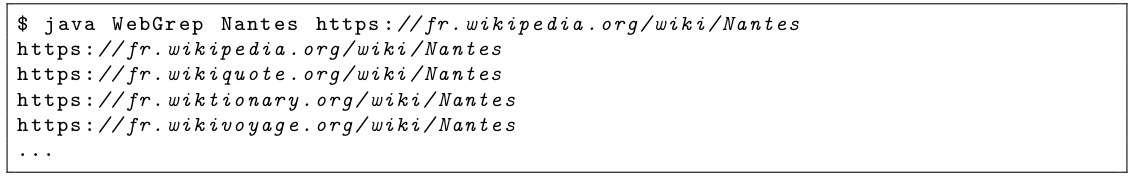
\includegraphics[width=.8\textwidth]{TP3.png}
   };

   \draw<3> (5.5,-1) node{\begin{minipage}{\textwidth}
     \begin{exampleblock}{Activités coopérantes}
        \begin{itemize}
        \item Interface réactive (compilation à la volée, \dots)
        \item Traitement de requêtes sur un serveur, \dots
        \end{itemize}
     \end{exampleblock}
     \begin{block}{Stratégie de parallélisation}
        \begin{itemize}
        \item Découper le problème en tâches indépendantes
        \item Associer des tâches à chaque c\oe ur 
        \item S'assurer que les c\oe urs collaborent correctement
        \end{itemize}
     \end{block}
      \end{minipage}
   };
   \end{tikzpicture}
\end{frame}

\mode<all>



\subsection{Programmation parallèle}
\mode*

\begin{frame} {Approches pour la programmation parallèle}
    \begin{shadequote}{C.A.R Hoare}
    A primary aim of an operating system is to share a computer installation among many programs making unpredictable demands upon its resources.
    \end{shadequote}

    \vfill

    \begin{block}{Processus versus thread}
        \begin{itemize}
        \item \alert{Informatique} = traitement auto\alert{matique} de l'\alert{informat}ion
        \item Le système d'exploitation abstrait le \alert{processeur} et la \alert{mémoire}
            \begin{description}\footnotesize
            \item[Processus :] contexte d'exécution d'un programme (partage de mémoire)
            \item[Thread :] description d'une exécution séquentielle (partage du processeur)
            \end{description}
        \item Chaque processus contient un ou plusieurs threads
        \end{itemize}
    \end{block}
\end{frame}

\begin{frame} {Approches pour la programmation parallèle}
    \begin{exampleblock}{Programmation multi-processus}
       \begin{itemize}
         \item Plusieurs processus, un thread par processus
         \item Communication par passage de messages
         \item Avantages : 
       \begin{description}
         \item [Robustesse :] les processus sont isolés les uns des autres par l'OS
         \item [Répartition :] on peut répartir les processus sur un réseau de machines (passage à l'échelle)
       \end{description}
       \end{itemize}
     \end{exampleblock}
        
    \vfill
    \begin{exampleblock}{Programmation multi-threads}
       \begin{itemize}
         \item Un seul processus, plusieurs threads au sein du même processus
         \item Communication par mémoire partagée
         \item Avantages : 
        \begin{description}
        \item [Efficacité :] données et références partagées (pas de copie) %communication et commutation de contexte en espace utilisateur.
        \item [Simplicité :] intégration presque transparente au sein des langages de programmation %(communication par référence et par valeur)
        \end{description}
       \end{itemize}
    \end{exampleblock}
\end{frame}

\begin{frame}{Intégration aux langages de programmation}
  
\vfill
  \begin{block}{Java}
        La JVM est une machine multi-thread. Le \texttt{GC} est un thread.

    \begin{description}
    \item[API historique] Définition de tâches, de threads et outils basiques pour la synchronisation
    \item[Depuis Java 5] La bibliothèque \href{https://docs.oracle.com/javase/8/docs/api/java/util/concurrent/package-summary.html}{\lstinline{java.util.concurrent}}
    repose en grande partie sur les travaux de Doug Lea (\url{http://gee.cs.oswego.edu/dl/index.html})
    \end{description}
    \end{block}
\vfill
\begin{block}{C++}
    Donne accès aux threads du système.
    \begin{description}
    \item[Avant C++11] accès direct aux threads système (\structure{POSIX pthread} et \structure{WINAPI thread} depuis les années 1990).
    \item[Depuis C++11] intégration d'une API à la bibliothèque standard.
    \end{description}
    \end{block}
\vfill

\end{frame}


\begin{frame}[fragile]{Tâche}

  \begin{itemize}
  \item Code exécuté par un thread.
  \end{itemize}

  \begin{exampleblock}{C++}
    N'importe quelle fonction (pointeur de fonction)
    \begin{lstlisting}[numbers=none]
  void printer (string message) {
    cout << message << endl;
  }
    \end{lstlisting}
  \end{exampleblock}

  \begin{exampleblock}{Java}
  Implémentation de l'interface fonctionnelle \lstinline{Runnable}
     \begin{lstlisting}[numbers=none]
  public record Printer (String message) implements Runnable {

    public void run () {
      System.out.println(message);
    }

  }
    \end{lstlisting}
\end{exampleblock}
\end{frame}


\begin{frame}[fragile]{Thread et contexte d'exécution}

  \begin{block}{Java : classe \lstinline{java.lang.Thread}}
     \begin{lstlisting}[numbers=none]
var task = new Printer("hello world");
//Runnable task = () -> System.out.println("hello world");
var thread = new Thread(task);
thread.start();
    \end{lstlisting}
    \end{block}

  \begin{block}{C++ : classe \lstinline{std::thread}}
    \begin{lstlisting}[numbers=none]
thread t(printer, "hello world");
// Started by constructor
   \end{lstlisting}
  \end{block}


  \begin{exampleblock}{Exemple}
    \begin{lstlisting}[numbers=none]
var messages = new String[]{"Hello", "Multithreaded", "World"};
for(var message : messages) {
  new Thread(()->System.out.print(message)).start();
}
   \end{lstlisting}
  \end{exampleblock}
\begin{citing}
\jitem \lstinline{cm1/HelloWorld.java}
\end{citing}
\end{frame}



\begin{frame}[fragile]
  \frametitle{Principales méthodes de la classe gérant les threads}

  \vfill
\begin{block}{Obtenir la référence sur le thread qui contrôle la tâche en cours}
   \structure{Java :} \lstinline|Thread.currentThread()| \hfill
   \structure{C++ :} \lstinline|std::this_thread|
\end{block}
\pause
  \vfill
  \vfill
\begin{block}{Endormir le thread \lstinline{t} pour \lstinline{ms} millisecondes}
   \structure{Java :} \lstinline|t.sleep(ms)| \hfill
   \structure{C++ :} \lstinline|t.sleep_for(std::chrono::milliseconds(ms))|
 \end{block}
  \vfill
  \vfill
\pause
\begin{block}{Attente de la terminaison d'un thread \lstinline{t}}
 \begin{description}
 \item[Java ou C++ :] \lstinline|t.join()|
  \item [\alert{ attention :}] en C++, un thread doit être détaché avant la terminaison du thread qui l'a lancé (\lstinline|t.detach()|). 
 \end{description}
\end{block}
  \vfill
\end{frame}

\begin{frame}[fragile]{Interrompre proprement un thread}

  \begin{alertblock}{Forcer un thread à s'arrêter}
  Impossible : \lstinline|public void stop()| est dépréciée !
  \end{alertblock}
  \vfill
  \begin{block}{Méthode \lstinline|public void interrupt()|}
    Demande la terminaison.
    \begin{itemize}
    \item Lève un drapeau booléen pour avertir le thread.
    \item La tâche peut (doit) vérifier régulièrement les demandes d'interruption
    \begin{itemize}
    \item \lstinline|public static boolean interrupted()| ou
    \item \lstinline|public boolean isInterrupted()|.
    \end{itemize}
  \item \lstinline|interrupted()| et \lstinline|isInterrupted()| rebaissent le drapeau.
  \item Si le thread est bloqué ou en attente,  \lstinline|InterruptedException| est lancée.
    \end{itemize}
  \end{block}
  \vfill
  \begin{exampleblock}{Pas d'équivalent en C++}
    Utiliser une variable booléenne comme drapeau.
  \end{exampleblock}
\end{frame}



\begin{frame}[fragile]{L'interface \texttt{ExecutorService}}

\begin{block}{Association tâche / contexte d'exécution}
  \texttt{java.util.concurrent} offre les outils pour construire \structure{simplement} des associations $n \leftrightarrow m$ avec différentes stratégies

  \begin{lstlisting}
public interface ExecutorService {
  void execute (Runnable task);
  Future<?> submit (Runnable task);
  Future<T> submit (Callable<T> task);
  List<Future<T>> invokeAll (Collection<Callable<T>> tasks)
    throws InterruptedException;
  T invokeAny (Collection<Callable<T>> tasks)
    throws InterruptedException, ExecutionException;
}
  \end{lstlisting}
\end{block}

  \begin{exampleblock}{Exemple}
  \begin{lstlisting}
var threadPool = Executors.newFixedThreadPool(5);
for(int i = 0; i < 50; ++i){
  threadPool.execute(() -> System.out.println(i));
}
  \end{lstlisting}
  \end{exampleblock}
  
\end{frame}


\begin{frame}[fragile]{Tâche retournant un résultat}

  \begin{block}{L'interface \lstinline{Callable}}
    Version générique d'une tâche qui retourne un résultat.

    \begin{lstlisting}[numbers=none]
public interface Callable<V> {
  V call() throws Exception;
}
    \end{lstlisting}
  \end{block}
  
  \bigskip

  \begin{block}{L'interface \lstinline{Future}}
    Version générique du résultat d'un calcul \textit{asynchrone}. 

    \begin{lstlisting}[numbers=none]
public interface Future<V> {
  boolean cancel( boolean evenIfRunning );
  V get() throws InterruptedException, ExecutionException;
  V get( long timeout, TimeUnit unit ) throws...;
  boolean isCancelled();
  boolean isDone();
}
    \end{lstlisting}
  \end{block}
\end{frame}

\begin{frame}[fragile]{Implémentations de \texttt{ExecutorService}}
  \begin{block}{Classe \lstinline{java.util.concurrent.Executors}}
    \textit{Factory} qui permet d'instancier simplement
    des \lstinline{ExecutorService}, dont :
    \begin{itemize}
    \item \structure{\lstinline{ThreadPoolExecutor} :} implante différentes variantes basées sur le concept de \textit{pool} de \lstinline{Thread} : \textit{single}, \textit{fixed}, \textit{cached}
    \item \structure{\lstinline{ScheduledThreadPoolExecutor} :} stratégie permettant de préciser un délai lors de la soumission, à écouler entre la soumission et le début de l'exécution de la tâche
    \item \structure{\lstinline{ForkJoinPool} :} stratégie particulière pour exécuter des \lstinline{ForkJoinTask}, qui créent elles-mêmes des tâches
    \item \structure{\lstinline{VirtualThreadPerTaskExecutor} :} ``green threads'' gérés par le langage et non par le système
    \end{itemize}
  \end{block}
\end{frame}

\begin{frame}{Quelle stratégie est la plus efficace ?}
  \begin{block}{Ça dépend de l'application !} 
    \begin{itemize}
    \item Trop peu de threads et on n'exploite pas les capacités de calcul. 
    \item Trop de threads et on perd du temps à leur manipulation.
    \end{itemize}
  \end{block}
  
  \begin{block}{Ça dépend de la plate-forme !}
    \begin{itemize}
    \item Machine : nombre de c{\oe}urs, hiérarchie mémoire, etc.
    \item OS : politique d'ordonnancement des threads côté noyau.
    \item JVM : implémentation des stratégies, politique d'ordonnancement des threads côté utilisateur.
    \end{itemize}
  \end{block}
  
  \begin{center}
  \alert{Mesurer les performances !}
  \end{center}
\end{frame}





\mode<all>



\subsection{Limites de la parallélisation}
\mode*

\begin{frame}{Limites de la parallélisation}
  \vFill
  \begin{center}
      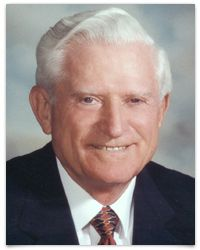
\includegraphics[height=4cm]{gene_amdahl}\\
      Gene M. Amdahl
    \end{center}
  \vFill
  \begin{citing}
  \item[A67] Gene M. Amdahl. \textit{Validity of the Single Processor Approach to Achieving Large-Scale Computing Capabilities.} AFIPS (1967)
  \end{citing}
\end{frame}
 
\begin{frame}{Limites de la parallélisation}
  \begin{alertblock}{Question}
    \begin{itemize}
    \item Un sondeur a besoin de 22 jours pour interroger 1000 sondés.
    \item Combien de temps faut-il à 22 sondeurs pour faire le même sondage ?
    \end{itemize}
  \end{alertblock}
  \pause
  \begin{alertblock}{Question}
    \begin{itemize}
    \item Une éléphante a besoin de 22 mois pour donner la vie.
    \item Combien de temps faut-il à 22 éléphantes pour faire le même éléphanteau ?
    \end{itemize}
  \end{alertblock}
  \pause
  \begin{block}{Cas géneral}
    \begin{itemize}
    \item Une proportion $p$ du programme peut être parallélisée.
    \item Une proportion $1-p$ ne le peut pas.
    \end{itemize}
  \end{block}
\end{frame}
 
\begin{frame}{La loi d'Amdahl}
    \begin{description}
    \item[$p$: ] Proportion du programme parallélisable 
    \item[$T(n)$: ] Temps nécessaire à $n$ threads
    \item[$S(n)$: ] Accélération (Speedup) $S(n) = \frac{T(1)}{T(n)}$ 
    \end{description}
    \pause
    \hspace{\fill}
    \begin{minipage}{.6\textwidth}
    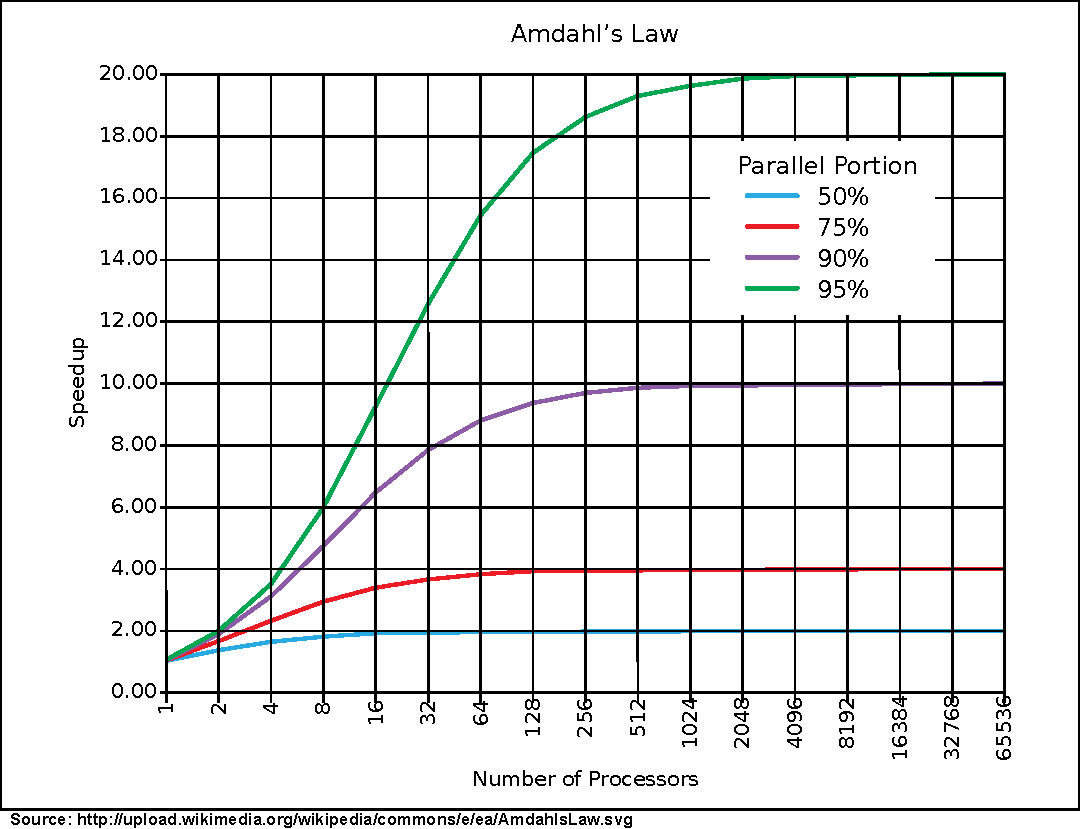
\includegraphics[width=\textwidth]{amdahl-law}
    \end{minipage}
    \hspace{\fill}
    \begin{minipage}{.35\textwidth}
      \vspace{-1cm}
      $$
      \begin{array}{rcl}
        \displaystyle S(n) &\displaystyle =& \displaystyle \frac{1}{1-p + \frac{p}{n}}\\
        \\
        \displaystyle S(n) &\displaystyle <& \displaystyle\frac{1}{1-p}\\
        \\
        \displaystyle \lim_{n\rightarrow \infty} S(n) &\displaystyle =& \displaystyle \frac{1}{1-p}
      \end{array}
      $$
    \end{minipage}
    \hspace{\fill}
\end{frame}
 
\begin{frame}{Limites de la loi d'Amdahl}
  \begin{block}{Hypothèses cachées :}
    \begin{itemize}
    \item Parallélisation imparfaite
    \begin{itemize}
    \item $p$ dépend des données (loi de Gustafson)
    \item $p$ dépend de l'algorithme
    \end{itemize}
    $$S_p(n) \le n$$
  \item Synchronisation non-parallélisable
    \begin{itemize}
    \item Gestion de la concurrence
    \end{itemize}
    $$S_c(n) \le 1$$
    \end{itemize}
  \end{block}
  \begin{block}{Formule plus réaliste}
    $$
    S(n) = \frac{1}{\frac{1-p}{S_c(n)} + \frac{p}{S_p(n)}} \le \frac{1}{1-p + \frac{p}{n}}
    $$
    \begin{center}
      \alert{Mesurez vos performances !}
    \end{center}
  \end{block}
\end{frame}



\mode<all>



\subsection{Introduction à la concurrence}
\mode*

\begin{frame}{Problématique du cours}
    \begin{shadequote}{Maurice Herlihy \& Nir Shavit}
    For many of the applications you may wish to parallelize, you will find that there are significant parts that can easily be determined
    as executable in parallel because they do not require any form of coordination or communication. However, (...)
    \alert{there is no cookbook recipe for identifying these parts}. This is where the application designer needs to use
    his or her accumulated understanding of the algorithm being parallelized. Luckily, in many cases it is obvious how to find such parts.
    
    \vspace{4mm}
    \alert{The more substantial problem} (...)
    \alert{is how to deal with the remaining parts of the program.} As noted earlier, these are the parts that cannot be easily parallelized
    because the program must access shared data and requires interprocess coordination and communication in an essential way.
    \end{shadequote}
\end{frame}

\begin{frame}{Du parallélisme à la concurrence}
\begin{center}
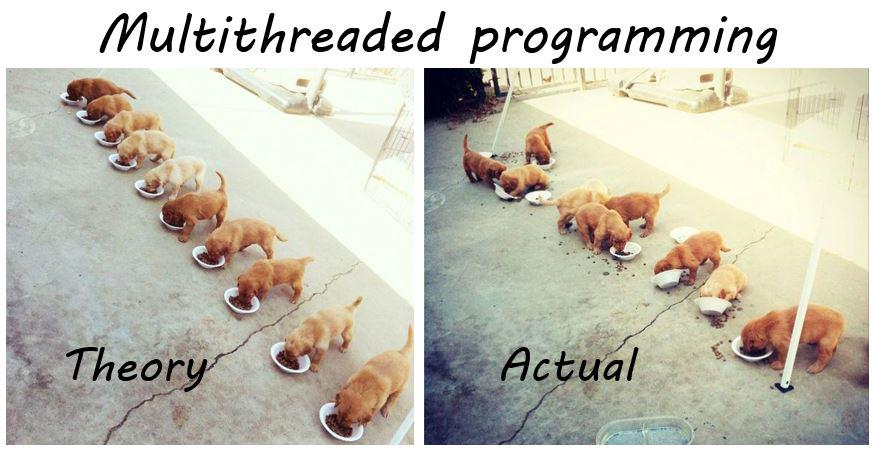
\includegraphics[width=\textwidth]{pupies}
\end{center}
\end{frame}


%%%%%%%%%%%%%%%%%%%%%%%%%%%%%%%%%%%%%%%%%%%%%%%%%%%%%%%%%%%%%%%%%%%%%%%%%

\begin{frame}{Parallélisme versus concurrence}
  \vFill
  \begin{block}{Principale difficulté}
    \begin{description}
    \item[Parallélisme :] Identifier les tâches indépendantes
    \item[Concurrence :] Gérer l'incertitude
    \end{description}
    \begin{shadequote}{Leslie Lamport}
    A distributed system is one in which the failure of a computer you didn't even know existed can render your own computer unusable.
    \end{shadequote}
  \end{block}
  \vFill
  \uncover<2->{
  \begin{block}{Contexte d'exécution}
    \begin{description}
    \item[Parallélisme :] Choisi en fonction du problème à résoudre
    \item[Concurrence :] Imposé \textit{a priori} par le problème
    \end{description}
  \end{block}
  }
  \vFill
  \uncover<3->{
  \begin{block}{Passage à l'échelle}
    \begin{minipage}{.5\textwidth}
      \begin{description}
      \item[Parallélisme :] $S_p(n) = \Omega(n)$
      \end{description}
    \end{minipage}\begin{minipage}{.45\textwidth}
      \begin{description}
      \item[Concurrence :] $S_c(n) = \Omega(1)$
      \end{description}
    \end{minipage}
  \end{block}
  }
  \vFill
  \begin{citing}
  \item[R15] Michel Raynal. \textit{Parallel Computing vs. Distributed Computing: A Great Confusion? (Position Paper).} Euro-Par Workshops (2015).
  \end{citing}
\end{frame}

\begin{frame}{Point vocabulaire}
  \begin{tabular}{ccc}
    &Une seule unité d'exécution & Plusieurs unités d'exécution
    \\
    
\begin{tikzpicture}
        \draw[white] (0, 0) rectangle (2,3);
        \draw (1, 1.75) node{Problème};
        \draw (1, 1.25) node{Séquentiel};
    \end{tikzpicture}
&
    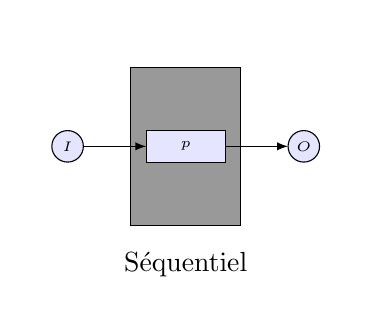
\begin{tikzpicture}

        \draw[white] (-0.5, -0.3) rectangle (3.5,3);
        \draw (1.5, 0) node{Séquentiel};

        \draw[fill=black!40] (0.8, 0.5) rectangle (2.2,2.5);
        \draw[fill=blue!10] (1.5, 1.5) +(-0.5, -.2) rectangle +(0.5, .2) +(0,0) node{\tiny $p$};

        \draw[-latex] (0.2, 1.5) -- (1,1.5);
        \draw[-latex] (2, 1.5) -- (2.8,1.5);

        \draw[fill=blue!10] (0, 1.5) circle (2mm) node{\tiny $I$};
        \draw[fill=blue!10] (3, 1.5) circle (2mm) node{\tiny $O$};
      \end{tikzpicture}
&
      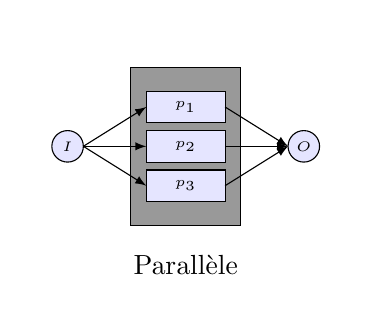
\begin{tikzpicture}
        \draw[white] (-0.5, -0.3) rectangle (3.5,3);
        \draw (1.5, 0) node{Parallèle};

        \draw[fill=black!40] (0.8, 0.5) rectangle (2.2,2.5);
        \draw[fill=blue!10] (1.5, 2) +(-0.5, -.2) rectangle +(0.5, .2)   +(0,0) node{\tiny $p_1$};
        \draw[fill=blue!10] (1.5, 1.5) +(-0.5, -.2) rectangle +(0.5, .2) +(0,0) node{\tiny $p_2$};
        \draw[fill=blue!10] (1.5, 1) +(-0.5, -.2) rectangle +(0.5, .2)   +(0,0) node{\tiny $p_3$};

        \draw[-latex] (0.2, 1.5) -- (1,2);
        \draw[-latex] (0.2, 1.5) -- (1,1.5);
        \draw[-latex] (0.2, 1.5) -- (1,1);

        \draw[-latex] (2, 2)   -- (2.8,1.5);
        \draw[-latex] (2, 1.5) -- (2.8,1.5);
        \draw[-latex] (2, 1)   -- (2.8,1.5);

        \draw[fill=blue!10] (0, 1.5) circle (2mm) node{\tiny $I$};
        \draw[fill=blue!10] (3, 1.5) circle (2mm) node{\tiny $O$};
      \end{tikzpicture}
    \\
    
\begin{tikzpicture}
        \draw[white] (0, 0) rectangle (2,3);
        \draw (1, 1.75) node{Problème};
        \draw (1, 1.35) node{de};
        \draw (1, 0.95) node{concurrence};
    \end{tikzpicture}
    &
      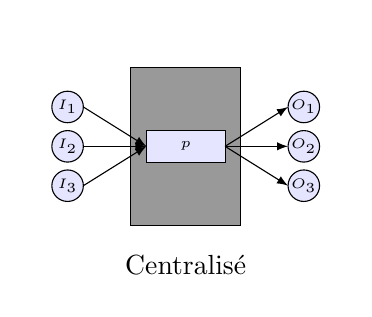
\begin{tikzpicture}
        \draw[white] (-0.5, -0.3) rectangle (3.5,3);
        \draw (1.5, 0) node{Centralisé};

        \draw[fill=black!40] (0.8, 0.5) rectangle (2.2,2.5);
        \draw[fill=blue!10] (1.5, 1.5) +(-0.5, -.2) rectangle +(0.5, .2) +(0,0) node{\tiny $p$};

        \draw[-latex] (0.2, 2) -- (1,1.5);
        \draw[-latex] (0.2, 1.5) -- (1,1.5);
        \draw[-latex] (0.2, 1) -- (1,1.5);

        \draw[-latex] (2, 1.5) -- (2.8,2);
        \draw[-latex] (2, 1.5) -- (2.8,1.5);
        \draw[-latex] (2, 1.5) -- (2.8,1);

        \draw[fill=blue!10] (0, 2) circle (2mm)   node{\tiny $I_1$};
        \draw[fill=blue!10] (0, 1.5) circle (2mm) node{\tiny $I_2$};
        \draw[fill=blue!10] (0, 1) circle (2mm)   node{\tiny $I_3$};

        \draw[fill=blue!10] (3, 2) circle (2mm)   node{\tiny $O_1$};
        \draw[fill=blue!10] (3, 1.5) circle (2mm) node{\tiny $O_2$};
        \draw[fill=blue!10] (3, 1) circle (2mm)   node{\tiny $O_3$};
      \end{tikzpicture}
      &
      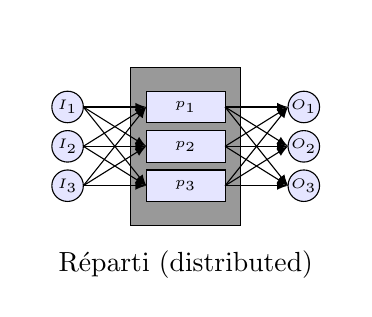
\begin{tikzpicture}
        \draw[white] (-0.5, -0.3) rectangle (3.5,3);
        \draw (1.5, 0) node{Réparti (distributed)};

        \draw[fill=black!40] (0.8, 0.5) rectangle (2.2,2.5);
        \draw[fill=blue!10] (1.5, 2) +(-0.5, -.2) rectangle +(0.5, .2)   +(0,0) node{\tiny $p_1$};
        \draw[fill=blue!10] (1.5, 1.5) +(-0.5, -.2) rectangle +(0.5, .2) +(0,0) node{\tiny $p_2$};
        \draw[fill=blue!10] (1.5, 1) +(-0.5, -.2) rectangle +(0.5, .2)   +(0,0) node{\tiny $p_3$};

        \draw[-latex] (0.2, 2) -- (1,2);
        \draw[-latex] (0.2, 2) -- (1,1.5);
        \draw[-latex] (0.2, 2) -- (1,1);

        \draw[-latex] (0.2, 1.5) -- (1,2);
        \draw[-latex] (0.2, 1.5) -- (1,1.5);
        \draw[-latex] (0.2, 1.5) -- (1,1);
                         
        \draw[-latex] (0.2, 1) -- (1,2);
        \draw[-latex] (0.2, 1) -- (1,1.5);
        \draw[-latex] (0.2, 1) -- (1,1);

        \draw[-latex] (2, 2)   -- (2.8,2);
        \draw[-latex] (2, 2)   -- (2.8,1.5);
        \draw[-latex] (2, 2)   -- (2.8,1);
                                    
        \draw[-latex] (2, 1.5) -- (2.8,2);
        \draw[-latex] (2, 1.5) -- (2.8,1.5);
        \draw[-latex] (2, 1.5) -- (2.8,1);
                                    
        \draw[-latex] (2, 1)   -- (2.8,2);
        \draw[-latex] (2, 1)   -- (2.8,1.5);
        \draw[-latex] (2, 1)   -- (2.8,1);

        \draw[fill=blue!10] (0, 2) circle (2mm)   node{\tiny $I_1$};
        \draw[fill=blue!10] (0, 1.5) circle (2mm) node{\tiny $I_2$};
        \draw[fill=blue!10] (0, 1) circle (2mm)   node{\tiny $I_3$};

        \draw[fill=blue!10] (3, 2) circle (2mm)   node{\tiny $O_1$};
        \draw[fill=blue!10] (3, 1.5) circle (2mm) node{\tiny $O_2$};
        \draw[fill=blue!10] (3, 1) circle (2mm)   node{\tiny $O_3$};
      \end{tikzpicture}
      \end{tabular}
\end{frame}

\begin{frame}{Exercice}

  \begin{alertblock}{Problème de parallélisme ou de concurrence ?}
    \begin{enumerate} 
    \item Éviter les collisions sur la route.
    \item Optimiser la vitesse de production d'une usine (Fordisme).
    \item Élire le président de la république.
    \item Massively multiplayer online role-playing game.
    \item Prévoir la météo.
    \item Les projets semestriels en groupe.
    \item Un orchestre symphonique.
    \end{enumerate} 
  \end{alertblock}
\end{frame}

\mode<all>



 
\section{Exécutions d'un programme concurrent}
\mode*


\subsection{Notion d'asynchronisme}

\begin{frame}[fragile]{Un premier exemple}

    \begin{lstlisting}[numbers=none]
var t1 = new Thread(() -> {
  System.out.print("Hello ");
  System.out.print("World ");
});
var t2 = new Thread(() -> {
  System.out.print("Multithreaded ");
});
 
t1.start();
t2.start();

t1.join();
t2.join();

System.out.println("!");
    \end{lstlisting}
\vfill
\begin{block}{Expérience}
   \begin{itemize}
      \item Lancer le programme plusieurs fois. Qu'observe-t-on ? 
   \end{itemize}
\end{block}
\begin{citing}
\jitem \lstinline{cm2/HappensBefore.java}
\end{citing}
\end{frame}



%%%%%%%%%%%%%%%%%%%%%%%%%%%%%%%%%%%%%%%%%%%%%%%%%%%%%%%%%%%%%%%%%%%%%%%%% 

\begin{frame}[fragile]{Non déterminisme des sorties du programme}

    \begin{block}{Une exécution possible}
%    \begin{itemize}
%    \item  Toute action a un instant de début et un instant de fin
%    \end{itemize}
\scalebox{.7}{
      \begin{tikzpicture}
        \draw[alertColor,   -latex] (0,2) node[left]{$t1$}   +(3.4,0) -- (8.5,2);
        \draw[structure,    -latex] (0,1) node[left]{$main$}          -- (13.4,1);
        \draw[exampleColor, -latex] (0,0) node[left]{$t2$}   +(3,0) -- (8,0);
        \draw[->] (0,-.5) node[left]{temps réel}   -- (13.4,-.5);

        \draw[structure   , fill=structure!20, rounded corners]    (1.5 ,1)  +(-.8,-0.3) rectangle +(.8,0.3) +(0,0) node{$t1.start()$};
        \draw[structure   , fill=structure!20, rounded corners]    (3.2 ,1)  +(-.8,-0.3) rectangle +(.8,0.3) +(0,0) node{$t2.start()$};
        \draw[structure   , fill=structure!20, rounded corners]    (6.6 ,1)  +(-2.5,-0.3) rectangle +(2.5,0.3) +(0,0) node{$t1.join()$};
        \draw[structure   , fill=structure!20, rounded corners]    (10  ,1)  +(-.8,-0.3) rectangle +(.8,0.3) +(0,0) node{$t2.join()$};
        \draw[structure   , fill=structure!20, rounded corners]    (11.9,1)  +(-1,-0.3) rectangle +(1,0.3) +(0,0) node{$println(!)$};

        \draw[alertColor  , fill=alertColor!20, rounded corners]   (4.9 ,2)  +(-1,-0.3) rectangle +(1,0.3) +(0,0) node{$print(hello)$};
        \draw[alertColor  , fill=alertColor!20, rounded corners]   (7.0 ,2)  +(-1,-0.3) rectangle +(1,0.3) +(0,0) node{$print(world)$};
        \draw[exampleColor, fill=exampleColor!20, rounded corners] (5.5 ,0)  +(-2,-0.3) rectangle +(2,0.3) +(0,0) node{$print(multithreaded)$};

        \end{tikzpicture}
}
  \end{block}

  \begin{block}{Asynchronisme}
    Il est impossible de prévoir la vitesse d'exécution :
    \begin{itemize}
    \item  d'un thread par rapport à un autre,
    \item  d'une portion de code exécutée par un thread par rapport à une autre,
    \item  d'une exécution d'un thread par rapport à une autre.
    \end{itemize}
  \end{block}
  \begin{alertblock}{Question}
    \begin{itemize}
    \item Un programme n'est correct que si toutes ses exécutions le sont.
    \item Comment raisonner sur les exécutions concurrentes ?
    \end{itemize}
  \end{alertblock}
\end{frame}

\subsection{Relation happened before}

\begin{frame}{Causalité et concurrence}
  \vfill
  \begin{center}
     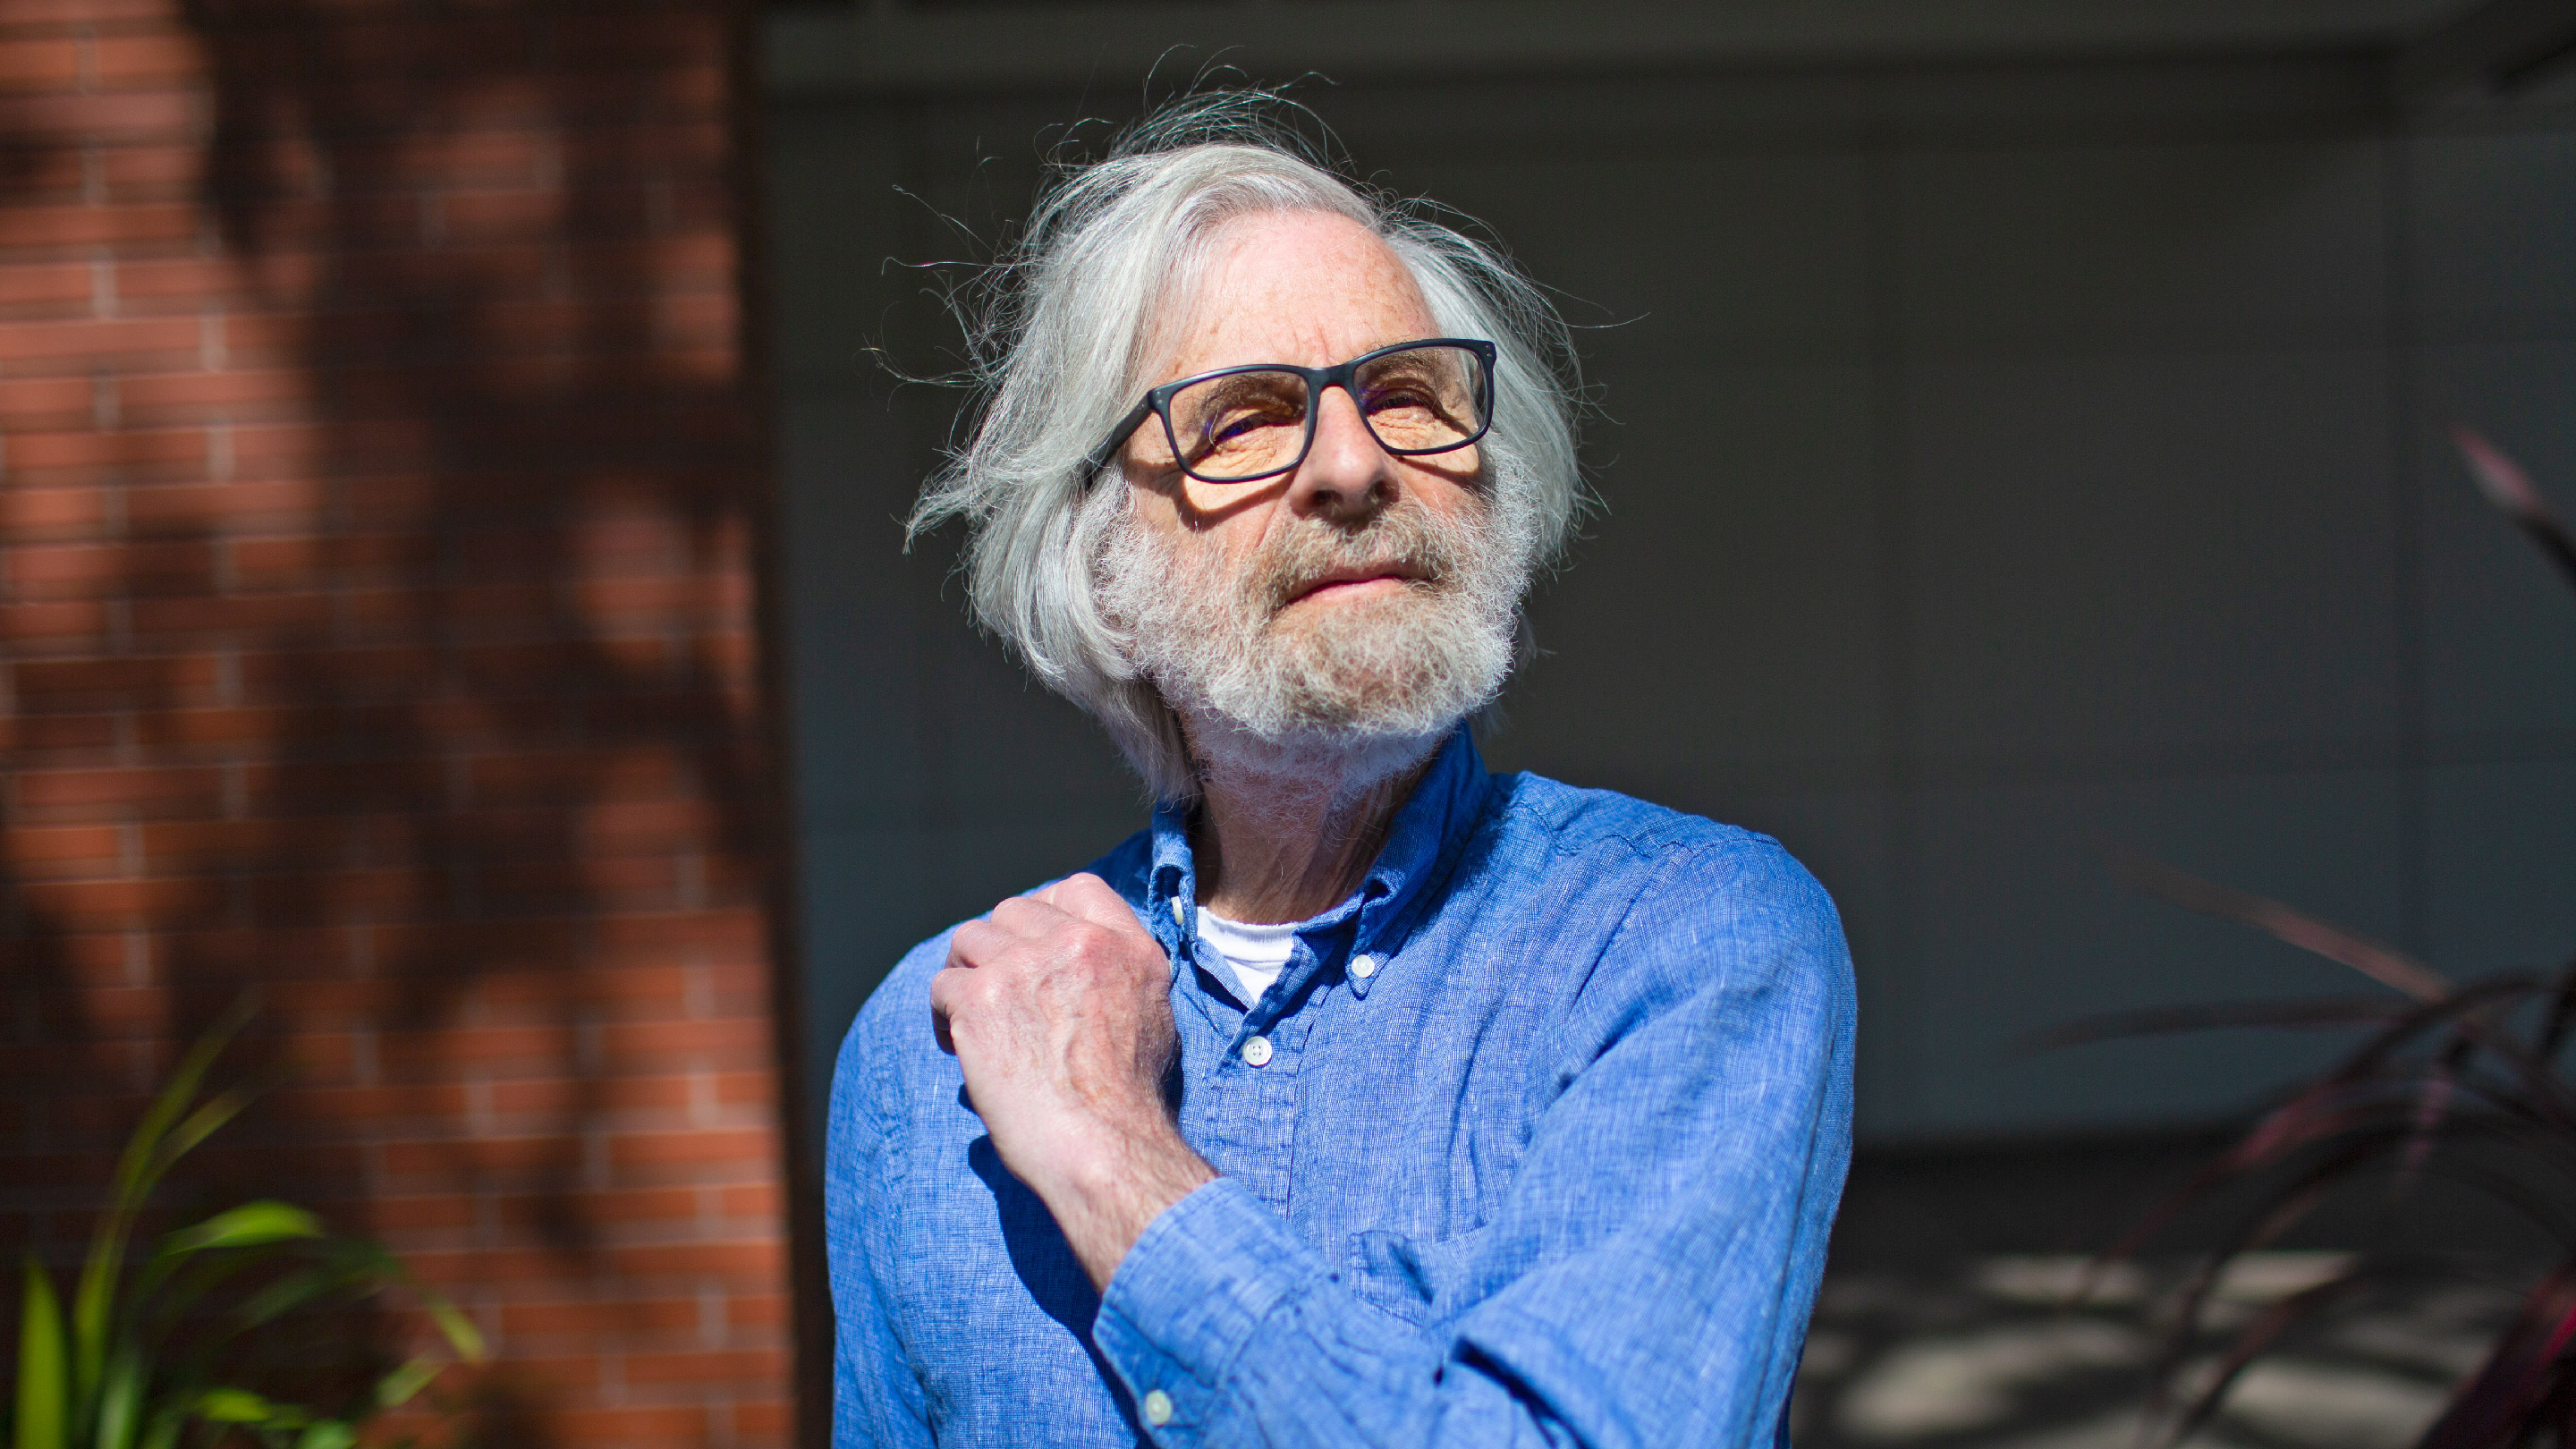
\includegraphics[height=5cm]{Lamport.jpg}\\
     Leslie Lamport\\
     Prix Turing 2013
  \end{center}
  \vfill
  \begin{citing}
  \item[L78] Leslie Lamport. \textit{Time, clocks, and the ordering of events in a distributed system.} CACM (1978)
  \item[L79] Leslie Lamport. \textit{How to make a multiprocessor computer that correctly executes multiprocess programs.} IEEE ToC (1979)
  \end{citing}
\end{frame}

\begin{frame}{La relation ``happened before'' (ordre causal)}
    \begin{shadequote}{Leslie Lamport}
    \small
    The \alert{concept of time} is fundamental to our way of
    thinking. \alert{It is derived} from the more basic concept of
    the \alert{order in which events occur}. (...)

    However, we will see that this concept must be carefully reexamined when considering events in a distributed system. (...)

    In a distributed system, it is sometimes impossible to
    say that one of two events occurred first. \alert{The relation
    "happened before" is therefore only a partial ordering
    of the events in the system.}
    \end{shadequote}

\begin{block}{Définitions}
    \begin{itemize}
    \item $e\mapsto e'$ si l'une des trois conditions s'applique :    
       \begin{itemize}
       \item \structure{Ordre de programme :} le même thread produit $e$ puis $e'$
       \item \structure{Précédence sémantique :} (précisé plus tard)
       \begin{itemize}
       \item Par exemple, $e = t.start()$ et $e'$ produit par $t$
       \item Par exemple, $e$ produit par $t$ et $e' = t.join()$
       \end{itemize}
       \item \structure{Transitivité :} $\exists e'', e\mapsto e'' \mapsto e'$
       \end{itemize}
    \item $e$ et $e'$ sont \structure{concurrents} $(e || e')$ si $e\not\mapsto e'$ et $e'\not\mapsto e$.
    \end{itemize}
    \end{block}
    \alert{Attention :} $\mapsto$ est seulement un ordre \alert{partiel} !

  \vfill
  \begin{citing}
  \item[L78] Leslie Lamport. \textit{Time, clocks, and the ordering of events in a distributed system.} CACM (1978)
  \end{citing}
\end{frame}

\begin{frame}{Exemple}
\begin{center}
\begin{tikzpicture}

   \draw[alertColor]   (0,1.5)   node[left]{$t1 :$};
   \draw[structure]    (0,1)   node[left]{$main :$};
   \draw[exampleColor] (0,0.5)   node[left]{$t2 :$};

   \draw[alertColor]   (3,1.5) node{\footnotesize$print(Hello)$};
   \draw[alertColor]   (5,1.5) node{\footnotesize$print(World)$};
   \draw[structure]    (.5,1) node{\footnotesize$main()$};
   \draw[structure]    (2,1)   node{\footnotesize$t1.start()$};
   \draw[structure]    (4,1) node{\footnotesize$t2.start()$};
   \draw[structure]    (6,1)   node{\footnotesize$t1.join()$};
   \draw[structure]    (7.5,1) node{\footnotesize$t2.join()$};
   \draw[structure]    (9.1,1)   node{\footnotesize$println(!)$};
   \draw[exampleColor] (5.75,0.5)   node{\footnotesize$print(Multithreaded)$};

   \draw[|->] (3.8,1.5) -- (4.2,1.5);
   \draw[|->, densely dotted] (1,1) -- (1.4,1);
   \draw[|->] (2.6,1) -- (3.4,1);
   \draw[|->] (4.6,1) -- (5.5,1);
   \draw[|->] (6.5,1) -- (6.9,1);
   \draw[|->] (8.1,1) -- (8.5,1);

   \draw[|->, rounded corners] (1.9,1.25) -- (1.9,1.5) -- (2.2,1.5);
   \draw[|->, rounded corners] (5.8,1.5) -- (6.1,1.5) -- (6.1,1.25);

   \draw[|->, rounded corners] (4,.75) -- (4,.5) -- (4.5,.5);
   \draw[|->, rounded corners] (7,.5) -- (7.5,.5) -- (7.5,.75);

   \end{tikzpicture}
   \end{center}
   \begin{block}{Observations}
     \begin{itemize}
     \item L'écriture ``Hello'' se produit avant l'écriture ``World'' 
     \item Les deux écritures de $t1$ sont concurrentes à l'écriture de $t2$ 
     \item Les trois se produisent avant l'écriture ``!''
     \end{itemize}
   \end{block}
\begin{block}{Projection sur l'objet \lstinline{System.out}}
\begin{center}
\begin{tikzpicture}

   \draw[alertColor]   (3,1.5) node{\footnotesize$print(Hello)$};
   \draw[alertColor]   (5,1.5) node{\footnotesize$print(World)$};
   \draw[structure]    (7,1)   node{\footnotesize$println(!)$};
   \draw[exampleColor] (4,0.5)   node{\footnotesize$print(Multithreaded)$};

   \draw[|->] (3.8,1.5) -- (4.2,1.5);

   \draw[|->, rounded corners] (5.8,1.5) -- (7,1.5) -- (7,1.25);
   \draw[|->, rounded corners] (5.3,.5) -- (7,.5) -- (7,.75);

   \end{tikzpicture}
   \end{center}
\end{block}
\end{frame}

\subsection{Cohérence séquentielle}

\begin{frame}[fragile]{Cohérence séquentielle}

\begin{block}{Il faudrait que...}
    \begin{shadequote}{Leslie Lamport}
    The result of any execution is the same as if the operations of all the processors were executed in some sequential order,
    and the operations of each individual processor appear in this sequence in the order specified by its program.
   \end{shadequote}
\end{block}
  \vfill
\begin{block}{Entrelacement}
        Un \structure{entrelacement} d'un ordre partiel $\le$ est un ordre total qui contient $\le$. 
\end{block}
\begin{block}{Cohérence séquentielle}
  Une exécution est \structure{séquentiellement cohérente} si son \structure{résultat observable} est \alert{le même que} celui d'un \structure{entrelacement} de son ordre ``happened before''.
\end{block}

\vfill
  \begin{citing}
  \item[L79] Leslie Lamport. \textit{How to make a multiprocessor computer that correctly executes multiprocess programs.} IEEE ToC (1979)
  \end{citing}
\end{frame}

\begin{frame}[fragile]{Exemple}

\begin{block}{Relation happened before}
\begin{center}
\begin{tikzpicture}

   \draw[alertColor]   (3,1.5) node{\footnotesize$print(Hello)$};
   \draw[alertColor]   (5,1.5) node{\footnotesize$print(World)$};
   \draw[structure]    (7,1)   node{\footnotesize$println(!)$};
   \draw[exampleColor] (4,0.5)   node{\footnotesize$print(Multithreaded)$};

   \draw[|->] (3.8,1.5) -- (4.2,1.5);

   \draw[|->, rounded corners] (5.8,1.5) -- (7,1.5) -- (7,1.25);
   \draw[|->, rounded corners] (5.3,.5) -- (7,.5) -- (7,.75);

   \end{tikzpicture}
\end{center}
\end{block}

\begin{block}{Entrelacements possibles}
  \begin{itemize}
   \item $\alert{print(Hello);~ } \alert{print(World);~ } {\color{exampleColor}print(Multithreaded);~ } \structure{println(!); }$
  \begin{description}
   \item[Résultat :] Hello World Multithreaded !
  \end{description}
   \item\vspace{2mm} $\alert{print(Hello);~ } {\color{exampleColor}print(Multithreaded);~ } \alert{print(World);~ } \structure{println(!); }$
  \begin{description}
   \item[Résultat :] Hello Multithreaded World !
  \end{description}
   \item\vspace{2mm} ${\color{exampleColor}print(Multithreaded);~ } \alert{print(Hello);~ } \alert{print(World);~ } \structure{println(!); }$
  \begin{description}
   \item[Résultat :] Multithreaded Hello World !
  \end{description}
  \end{itemize}
\end{block}
\end{frame}

\subsection{Machine à états d'un programme}

\begin{frame}[fragile]{Machine à états d'un programme}

Si l'exécution est séquentiellement cohérente, l'ensemble des exécutions est défini par une machine à états non-déterministe.

\begin{block}{États du système}
  À chaque instant, la \alert{configuration globale} est définie par :
  \begin{itemize}
    \item Un ensemble de threads
    \item L'état local de chaque thread
      \begin{itemize}
        \item valeur de ses variables locales
        \item prochaine instruction à exécuter
        \item peut-il exécuter sa prochaine instruction ? 
      \end{itemize}
    \item L'état de la mémoire
      \begin{itemize}
        \item ensemble de variables partagées
        \item valeur de chacune d'entre elles
      \end{itemize}
  \end{itemize}
  \end{block}

  \begin{block}{Transitions}
    Un \alert{ordonnanceur} décide quel thread exécutera sa prochaine instruction.
  \end{block}
\end{frame}

\begin{frame}{Machine à états de l'exemple}
\begin{center}
\begin{tikzpicture}

   \draw[fill=black!10, ultra thin, rounded corners] (-3,6)    +(-.5,-.15) rectangle +(1.1,.15);
   \draw[structure]    (-3,6)   node[left]{\tiny$main$} node {\tiny:} node[right]{\tiny$main()$};

   \draw[fill=black!10, ultra thin, rounded corners] (0,6)    +(-.5,-.35) rectangle +(1.1,.35);
   \draw[structure]    (0,6.2)  node[left]{\tiny$main$} node {\tiny:} node[right]{\tiny$t1.start()$};
   \draw               (0,6)    node[left]{\tiny$t1$} node {\tiny:} node[right]{\tiny\textsc{new}};
   \draw               (0,5.8)  node[left]{\tiny$t2$} node {\tiny:} node[right]{\tiny\textsc{new}};
                   
   \draw[fill=black!10, ultra thin, rounded corners] (0,5)    +(-.5,-.35) rectangle +(1.1,.35);
   \draw[structure]    (0,5.2)  node[left]{\tiny$main$} node {\tiny:} node[right]{\tiny$t2.start()$};
   \draw[alertColor]        (0,5)    node[left]{\tiny$t1$} node {\tiny:} node[right]{\tiny$print(hello)$};
   \draw               (0,4.8)  node[left]{\tiny$t2$} node {\tiny:} node[right]{\tiny\textsc{new}};
                   
   \draw[fill=black!10, ultra thin, rounded corners] (3,4.5)    +(-.5,-.35) rectangle +(1.1,.35);
   \draw[structure]    (3,4.7)  node[left]{\tiny$main$} node {\tiny:} node[right]{\tiny$t2.start()$};
   \draw[alertColor]        (3,4.5)  node[left]{\tiny$t1$} node {\tiny:} node[right]{\tiny$print(world)$};
   \draw               (3,4.3)  node[left]{\tiny$t2$} node {\tiny:} node[right]{\tiny\textsc{new}};

   \draw[fill=black!10, ultra thin, rounded corners] (6,4.0)    +(-.5,-.35) rectangle +(1.1,.35);
   \draw[structure]    (6,4.2)  node[left]{\tiny$main$} node {\tiny:} node[right]{\tiny$t2.start()$};
   \draw               (6,4.0)  node[left]{\tiny$t1$} node {\tiny:} node[right]{\tiny\textsc{terminated}};
   \draw               (6,3.8)  node[left]{\tiny$t2$} node {\tiny:} node[right]{\tiny\textsc{new}};

   \draw[fill=black!10, ultra thin, rounded corners] (0,4)    +(-.5,-.35) rectangle +(1.1,.35);
   \draw               (0,4.2)  node[left]{\tiny$main$} node {\tiny:} node[right]{\tiny$t1.join()$};
   \draw[alertColor]        (0,4)    node[left]{\tiny$t1$} node {\tiny:} node[right]{\tiny$print(hello)$};
   \draw[exampleColor] (0,3.8)  node[left]{\tiny$t2$} node {\tiny:} node[right]{\tiny$print(multi.)$};

   \draw[fill=black!10, ultra thin, rounded corners] (-3,3.5)    +(-.5,-.35) rectangle +(1.1,.35);
   \draw               (-3,3.7) node[left]{\tiny$main$} node {\tiny:} node[right]{\tiny$t1.join()$};
   \draw[alertColor]        (-3,3.5) node[left]{\tiny$t1$} node {\tiny:} node[right]{\tiny$print(hello)$};
   \draw               (-3,3.3) node[left]{\tiny$t2$} node {\tiny:} node[right]{\tiny\textsc{terminated}};

   \draw[fill=black!10, ultra thin, rounded corners] (3,3.5)    +(-.5,-.35) rectangle +(1.1,.35);
   \draw               (3,3.7)  node[left]{\tiny$main$} node {\tiny:} node[right]{\tiny$t1.join()$};
   \draw[alertColor]        (3,3.5)  node[left]{\tiny$t1$} node {\tiny:} node[right]{\tiny$print(world)$};
   \draw[exampleColor] (3,3.3)  node[left]{\tiny$t2$} node {\tiny:} node[right]{\tiny$print(multi.)$};

   \draw[fill=black!10, ultra thin, rounded corners] (6,3.0)    +(-.5,-.35) rectangle +(1.1,.35);
   \draw[structure]    (6,3.2)  node[left]{\tiny$main$} node {\tiny:} node[right]{\tiny$t1.join()$};
   \draw               (6,3.0)  node[left]{\tiny$t1$} node {\tiny:} node[right]{\tiny\textsc{terminated}};
   \draw[exampleColor] (6,2.8)  node[left]{\tiny$t2$} node {\tiny:} node[right]{\tiny$print(multi.)$};

   \draw[fill=black!10, ultra thin, rounded corners] (0,3)    +(-.5,-.35) rectangle +(1.1,.35);
   \draw               (0,3.2)  node[left]{\tiny$main$} node {\tiny:} node[right]{\tiny$t1.join()$};
   \draw[alertColor]        (0,3  )  node[left]{\tiny$t1$} node {\tiny:} node[right]{\tiny\tiny$print(world)$};
   \draw               (0,2.8)  node[left]{\tiny$t2$} node {\tiny:} node[right]{\tiny\textsc{terminated}};

   \draw[fill=black!10, ultra thin, rounded corners] (3,2.5)    +(-.5,-.35) rectangle +(1.1,.35);
   \draw[structure]    (3,2.7)  node[left]{\tiny$main$} node {\tiny:} node[right]{\tiny$t1.join()$};
   \draw               (3,2.5)  node[left]{\tiny$t1$} node {\tiny:} node[right]{\tiny\textsc{terminated}};
   \draw               (3,2.3)  node[left]{\tiny$t2$} node {\tiny:} node[right]{\tiny\textsc{terminated}};
 
   \draw[fill=black!10, ultra thin, rounded corners] (6,2.0)    +(-.5,-.35) rectangle +(1.1,.35);
   \draw               (6,2.2)  node[left]{\tiny$main$} node {\tiny:} node[right]{\tiny$t2.join()$};
   \draw               (6,2.0)  node[left]{\tiny$t1$} node {\tiny:} node[right]{\tiny\textsc{terminated}};
   \draw[exampleColor] (6,1.8)  node[left]{\tiny$t2$} node {\tiny:} node[right]{\tiny$print(multi.)$};

   \draw[fill=black!10, ultra thin, rounded corners] (3,1.5)    +(-.5,-.35) rectangle +(1.1,.35);
   \draw[structure]    (3,1.7)  node[left]{\tiny$main$} node {\tiny:} node[right]{\tiny$t2.join()$};
   \draw               (3,1.5)  node[left]{\tiny$t1$} node {\tiny:} node[right]{\tiny\textsc{terminated}};
   \draw               (3,1.3)  node[left]{\tiny$t2$} node {\tiny:} node[right]{\tiny\textsc{terminated}};

   \draw[fill=black!10, ultra thin, rounded corners] (3,0.5)    +(-.5,-.35) rectangle +(1.1,.35);
   \draw[structure]    (3,0.7)  node[left]{\tiny$main$} node {\tiny:} node[right]{\tiny$print(!)$};
   \draw               (3,0.5)  node[left]{\tiny$t1$} node {\tiny:} node[right]{\tiny\textsc{terminated}};
   \draw               (3,0.3)  node[left]{\tiny$t2$} node {\tiny:} node[right]{\tiny\textsc{terminated}};

   \draw[fill=black!10, ultra thin, rounded corners] (6,0.5)    +(-.55,-.2) rectangle +(1.15,.2);
   \draw[fill=black!10, ultra thin, rounded corners] (6,0.5)    +(-.5,-.15) rectangle +(1.1,.15);
   \draw               (6,0.5)  node[left]{\tiny$main$} node {\tiny:} node[right]{\tiny\textsc{terminated}};


   \draw[-latex]    (-2.7,6.5) -- (-2.7,6.15) ;
   \draw[structure, -latex, densely dotted]    (-1.9,6) -- (-.5,6) ;
   \draw[structure, -latex]    (0.3,5.65) -- (0.3,5.35) ;
   \draw[structure, -latex]    (0.3,4.65) -- (0.3,4.35) ;
   \draw[structure, -latex]    (3.3,4.15) -- (3.3,3.85) ;
   \draw[structure, -latex]    (3.3,2.15) -- (3.3,1.85) ;
   \draw[structure, -latex]    (3.3,1.15) -- (3.3,0.85) ;
   \draw[structure, -latex]    (6.3,3.65) -- (6.3,3.35) ;
   \draw[structure, -latex]    (6.3,2.65) -- (6.3,2.35) ;
   \draw[structure, -latex]    (4.1,.5) -- (5.45,.5) ;  \draw[structure] (4.75,.5) node[above]{\scriptsize!} ;

   \draw[exampleColor, -latex] (2.5,3.4) -- (1.1,3.1) ;  \draw[exampleColor] (1.6,3.25) node[above]{\scriptsize multithreaded} ;
   \draw[exampleColor, -latex] (-.5,3.9) -- (-1.9,3.6);  \draw[exampleColor] (-1.4,3.75) node[above]{\scriptsize multithreaded} ;
   \draw[exampleColor, -latex] (5.5,2.9) -- (4.1,2.6) ;  \draw[exampleColor] (4.6,2.75) node[above]{\scriptsize multithreaded} ;
   \draw[exampleColor, -latex] (5.5,1.9) -- (4.1,1.6) ;  \draw[exampleColor] (4.6,1.75) node[above]{\scriptsize multithreaded} ;

   \draw[alertColor, -latex] (-1.9,3.4) -- (-.5,3.1);  \draw[alertColor] (-1.2,3.25) node[above]{\scriptsize hello} ;
   \draw[alertColor, -latex] (1.1,4.9) -- (2.5,4.6) ;  \draw[alertColor] (1.8,4.75) node[above]{\scriptsize hello} ;
   \draw[alertColor, -latex] (1.1,3.9) -- (2.5,3.6) ;  \draw[alertColor] (1.8,3.75) node[above]{\scriptsize hello} ;
   \draw[alertColor, -latex] (1.1,2.9) -- (2.5,2.6) ;  \draw[alertColor] (1.8,2.75) node[above]{\scriptsize world} ;
   \draw[alertColor, -latex] (4.1,4.4) -- (5.5,4.1) ;  \draw[alertColor] (4.8,4.25) node[above]{\scriptsize world} ;
   \draw[alertColor, -latex] (4.1,3.4) -- (5.5,3.1) ;  \draw[alertColor] (4.8,3.25) node[above]{\scriptsize world} ;


   \end{tikzpicture}
\end{center}
\end{frame}

\begin{frame}{Mise en garde}
  \begin{shadequote}{John Carmack}
    A large fraction of the flaws in software development are due to programmers not fully understanding all the possible states their code may execute in.

    \structure{In a multithreaded environment}, the lack of understanding and the resulting problems are greatly amplified, \structure{almost to the point of panic if you are paying attention}.
  \end{shadequote}

\begin{alertblock}{Limitation des états mutables partagés}
\begin{itemize}
\item Identifier les objets partagés
\begin{itemize}
\item En minimiser l'utilisation
\item S'assurer qu'ils sont \textit{thread-safe}
\end{itemize}
\item Utiliser des structures de données immuables
\begin{itemize}
\item Éliminer les accesseurs
\item Déclarer les champs \lstinline{final}
\end{itemize}
\item Favoriser les fonctions pures
\end{itemize}
\end{alertblock}        

\end{frame}


\mode<all>



 
\section{Synchronisation bloquante}
\subsection{Section critique et verrouillage}
\mode*

\begin{frame}[fragile]{Exemple de programme parallèle}
  \begin{block}{Calcul de $\pi$ par la méthode de Monte-Carlo}
    \begin{center}
      \begin{tikzpicture}
        \draw[->] (0,-0.5) -- (0,2.5);
        \draw[->] (-0.5,0) -- (2.5,0);

        \draw[fill=alertColor!30] (0,0) rectangle (2,2);
        \draw[fill=exampleColor!30] (0,0) -- (2,0) arc (0:90:2) -- (0,0);
        \draw[alertColor] (1.7,1.7) node{$\mathcal{A_\mathcal{C}}$};
        \draw[exampleColor] (0.3,0.3) node{$\mathcal{A_\mathcal{D}}$};
        \draw (0,2) node[left]{1};
        \draw (2,0) node[below]{1};
        \draw (0,0) node[below left]{0};
        \draw (2.5,1.5) node[right]{$\mathcal{A_\mathcal{C}} = 1$};
        \draw (2.5,1) node[right]{$\mathcal{A_\mathcal{D}} = \frac{\pi}{4}$};
        \draw (2.5,0.5) node[right]{$\pi = 4\times \mathbb{P}(x^2 + y^2 < 1 | (x, y) \in [0; 1]^2) $};
      \end{tikzpicture}
    \end{center}
  \end{block}
  \begin{exampleblock}{Expérience}
    \begin{itemize}
    \item Tirer \lstinline{nbIterations} points dans l'intervalle $[0; 1]^2$
    \item Paralléliser entre \lstinline{nbThreads} threads
    \item Mesurer le temps d'exécution en fonction de \lstinline{nbIterations} et \lstinline{nbThreads}
    \end{itemize}
  \end{exampleblock}
\begin{citing}
\jitem Comparer \lstinline{cm3/Pi1_Sequential.java} et \lstinline{cm3/Pi2_Parallel.java}
\end{citing}
\end{frame}


\begin{frame}[fragile]{Tirer des nombres aléatoires en Java}
  \begin{shadequote}{Javadoc de \lstinline{java.util.Random}}
    Instances of \lstinline{java.util.Random} are threadsafe.
    However, the concurrent use of the same \lstinline{java.util.Random}
    instance across threads may encounter contention and consequent poor performance.
    Consider instead using \lstinline{ThreadLocalRandom} in multithreaded designs.
  \end{shadequote}

  \begin{block}{Définition -- thread safety}
    Un objet est \structure{thread safe} s'il a été conçu pour s'exécuter dans un environnement concurrent

    \begin{itemize}
    \item Pas de spécification formelle
    \item Tout objet partagé entre plusieurs threads doit être thread-safe
    \item Tout objet immutable est thread-safe
    \item Tout objet mutable thread-safe a des coûts liés à la synchronisation
    \end{itemize}
  \end{block}

\end{frame}



\begin{frame}[fragile]{Expérience : 8 threads tirent 10 000 000 pièces}
\vspace{-2mm}
\begin{enumerate}
\item Expérience : \uncover<2->{\structure{$7736ms$}}

\vspace{-3mm}
  \begin{tikzpicture}
    \fill[structure!20, rounded corners] (2.45,5.54) rectangle (6.95,5.84);
    \draw (5,5) node{\begin{minipage}{5cm}\begin{lstlisting}[numbers=none]
var random = new Random();
for(int i = 0; i < 8; i++) new Thread(() -> {
  for(int j = 0; j < 10000000; j++)
    random.nextBoolean();
}).start();
\end{lstlisting}\end{minipage}};
  \end{tikzpicture}

  \vspace{-2mm}
\item Expérience : \uncover<2->{\structure{$126ms$}}

\vspace{-3mm}
  \begin{tikzpicture}
    \fill[structure!20, rounded corners] (2.8,5.2) rectangle (7.31,5.5);
    \draw (5,5) node{\begin{minipage}{5cm}\begin{lstlisting}[numbers=none]
for(int i = 0; i < 8; i++) new Thread(() -> {
  var random = new Random();
  for(int j = 0; j < 10000000; j++)
    random.nextBoolean();
}).start();
\end{lstlisting}\end{minipage}};
  \end{tikzpicture}

\vspace{-2mm}
\item Expérience : \uncover<2->{\structure{$17ms$}}

\vspace{-3mm}
  \begin{tikzpicture}
    \fill[structure!20, rounded corners] (2.8,5.2) rectangle (10,5.5);
    \draw (5,5) node{\begin{minipage}{5cm}\begin{lstlisting}[numbers=none]
for(int i = 0; i < 8; i++) new Thread(() -> {
  var random = ThreadLocalRandom.current();
  for(int j = 0; j < 10000000; j++)
    random.nextBoolean();
}).start();
\end{lstlisting}\end{minipage}};
  \end{tikzpicture}
\end{enumerate}

\vspace{-2mm}
  \begin{citing}
  \jitem \lstinline{cm3/RandomExperiment.java}
  \end{citing}
\end{frame}



\begin{frame}[fragile]{Retour sur le calcul de $\pi$}
  \vfill
\vspace{-3mm}
  \begin{tikzpicture}
    \fill[structure!20, rounded corners] (3.6,4.3) rectangle (11.2,6.4);
    \fill[alertColor!20, rounded corners] (5.9,8.0) rectangle (7.9,8.3);
    \fill[alertColor!20, rounded corners] (7.3,4.7) rectangle (9.1,5);
    \fill[alertColor!20, rounded corners] (6.2,2.0) rectangle (7.4,2.3);
    \draw (5,5) node{\begin{minipage}{5cm}\begin{lstlisting}[numbers=none]
private static int result = 0;

public void pi(int nbThreads, int nbIterations) {
  threads = new Thread[n];
  for(int i = 0; i<nbThreads; i++) {
     threads[i] = new Thread(() -> {
       var random = ThreadLocalRandom.current();
       for(int i = 0; i<nbIterations; i++) {
         double x = random.nextDouble();
	 double y = random.nextDouble();
	 if(x*x + y*y < 1) result++;
       }
     });
  }
   
  for(var t : threads) t.start();
  for(var t : threads) t.join();
   
  System.out.println(result);
}
\end{lstlisting}\end{minipage}};
  \end{tikzpicture}
  \vfill
\begin{citing}
\jitem \lstinline{cm3/Pi3_ThreadLocalRandom.java}
\end{citing}
\end{frame}

\begin{frame}[fragile]{Explications}
  \begin{block}{Code simplifié}
\vspace{-3mm}
\begin{lstlisting}[numbers=none]
class Task implements Runnable {
  static int result = 0;
  public void run() {
    result++;
  }
}
\end{lstlisting}
\color{exampleColor}{On lance deux fois la tâche en parallèle, que devrait valoir \lstinline{result} à la fin ?}
  \end{block}
\pause
\vfill
  \begin{block}{Code décompilé : \lstinline[language=bash]{javap -c Task.class}}
  \vspace{-3mm}
\begin{verbatim}
public void run();
   Code:
      0: getstatic   #2    // Field result:I
      3: iconst_1
      4: iadd
      5: putstatic   #2    // Field result:I
      8: return
\end{verbatim}
  \end{block}
\end{frame}

\begin{frame}{Ce que l'on a}
\begin{center}
\begin{tikzpicture}

   \draw[fill=black!10, ultra thin, rounded corners]
     (0,6)    +(-.6,-.35) rectangle +(.7,.35);
   \draw[exampleColor]
     (0,6)  +(0,.2)   node[left]{\tiny$t1$}    node {\tiny:} node[right]{\tiny$\mathit{get()}$};
   \draw[alertColor]
     (0,6)  +(0,0)    node[left]{\tiny$t2$}    node {\tiny:} node[right]{\tiny$\mathit{get()}$};
   \draw
     (0,6)  +(0,-.2)  node[left]{\tiny$result$} node {\tiny=} node[right]{\tiny 0};

   \draw[fill=black!10, ultra thin, rounded corners]
     (2,6)    +(-.6,-.35) rectangle +(.7,.35);
   \draw[exampleColor]
     (2,6)  +(0,.2)   node[left]{\tiny$t1$}    node {\tiny:} node[right]{\tiny$\mathit{put(1)}$};
   \draw[alertColor]
     (2,6)  +(0,0)    node[left]{\tiny$t2$}    node {\tiny:} node[right]{\tiny$\mathit{get()}$};
   \draw
     (2,6)  +(0,-.2)  node[left]{\tiny$result$} node {\tiny=} node[right]{\tiny 0};

   \draw[fill=black!10, ultra thin, rounded corners]
     (6,6)    +(-.6,-.35) rectangle +(.7,.35);
   \draw
     (6,6)  +(0,.2)   node[left]{\tiny$t1$}    node {\tiny:} node[right]{\tiny$\textsc{term.}$};
   \draw[alertColor]
     (6,6)  +(0,0)    node[left]{\tiny$t2$}    node {\tiny:} node[right]{\tiny$\mathit{get()}$};
   \draw
     (6,6)  +(0,-.2)  node[left]{\tiny$result$} node {\tiny=} node[right]{\tiny 1};

%%%%%%%%%%%%%%%%%%%%%%%%%%%%%%%%%%%%%%%%%%%%%%%%%%%%%%%%%%
   \draw[fill=black!10, ultra thin, rounded corners]
     (0,5)    +(-.6,-.35) rectangle +(.7,.35);
   \draw[exampleColor]
     (0,5)  +(0,.2)   node[left]{\tiny$t1$}    node {\tiny:} node[right]{\tiny$\mathit{get()}$};
   \draw[alertColor]
     (0,5)  +(0,0)    node[left]{\tiny$t2$}    node {\tiny:} node[right]{\tiny$\mathit{put(1)}$};
   \draw
     (0,5)  +(0,-.2)  node[left]{\tiny$result$} node {\tiny=} node[right]{\tiny 0};

   \draw[fill=black!10, ultra thin, rounded corners]
     (2,5)    +(-.6,-.35) rectangle +(.7,.35);
   \draw[exampleColor]
     (2,5)  +(0,.2)   node[left]{\tiny$t1$}    node {\tiny:} node[right]{\tiny$\mathit{put(1)}$};
   \draw[alertColor]
     (2,5)  +(0,0)    node[left]{\tiny$t2$}    node {\tiny:} node[right]{\tiny$\mathit{put(1)}$};
   \draw
     (2,5)  +(0,-.2)  node[left]{\tiny$result$} node {\tiny=} node[right]{\tiny 0};

   \draw[fill=black!10, ultra thin, rounded corners]
     (4,5)    +(-.6,-.35) rectangle +(.7,.35);
   \draw
     (4,5)  +(0,.2)   node[left]{\tiny$t1$}    node {\tiny:} node[right]{\tiny$\textsc{term.}$};
   \draw[alertColor]
     (4,5)  +(0,0)    node[left]{\tiny$t2$}    node {\tiny:} node[right]{\tiny$\mathit{put(1)}$};
   \draw
     (4,5)  +(0,-.2)  node[left]{\tiny$result$} node {\tiny=} node[right]{\tiny 1};

   \draw[fill=black!10, ultra thin, rounded corners]
     (6,5)    +(-.6,-.35) rectangle +(.7,.35);
   \draw
     (6,5)  +(0,.2)   node[left]{\tiny$t1$}    node {\tiny:} node[right]{\tiny$\textsc{term.}$};
   \draw[alertColor]
     (6,5)  +(0,0)    node[left]{\tiny$t2$}    node {\tiny:} node[right]{\tiny$\mathit{put(2)}$};
   \draw
     (6,5)  +(0,-.2)  node[left]{\tiny$result$} node {\tiny=} node[right]{\tiny 1};

%%%%%%%%%%%%%%%%%%%%%%%%%%%%%%%%%%%%%%%%%%%%%%%%%%%%%%%%%%

   \draw[fill=black!10, ultra thin, rounded corners]
     (2,4)    +(-.6,-.35) rectangle +(.7,.35);
   \draw[exampleColor]
     (2,4)  +(0,.2)   node[left]{\tiny$t1$}    node {\tiny:} node[right]{\tiny$\mathit{put(1)}$};
   \draw
     (2,4)  +(0,0)    node[left]{\tiny$t2$}    node {\tiny:} node[right]{\tiny$\textsc{term.}$};
   \draw
     (2,4)  +(0,-.2)  node[left]{\tiny$result$} node {\tiny=} node[right]{\tiny 1};

   \draw[alertColor, fill=alertColor!20, ultra thin, rounded corners]
     (4,4)    +(-.65,-.4) rectangle +(.75,.4);
   \draw[alertColor, fill=alertColor!20, ultra thin, rounded corners]
     (4,4)    +(-.6,-.35) rectangle +(.7,.35);
   \draw
     (4,4)  +(0,.2)   node[left]{\tiny$t1$}    node {\tiny:} node[right]{\tiny$\textsc{term.}$};
   \draw
     (4,4)  +(0,0)    node[left]{\tiny$t2$}    node {\tiny:} node[right]{\tiny$\textsc{term.}$};
   \draw
     (4,4)  +(0,-.2)  node[left]{\tiny$result$} node {\tiny=} node[right]{\tiny 1};

%%%%%%%%%%%%%%%%%%%%%%%%%%%%%%%%%%%%%%%%%%%%%%%%%%%%%%%%%%

   \draw[fill=black!10, ultra thin, rounded corners]
     (0,3)    +(-.6,-.35) rectangle +(.7,.35);
   \draw[exampleColor]
     (0,3)  +(0,.2)   node[left]{\tiny$t1$}    node {\tiny:} node[right]{\tiny$\mathit{get()}$};
   \draw
     (0,3)  +(0,0)    node[left]{\tiny$t2$}    node {\tiny:} node[right]{\tiny$\textsc{term.}$};
   \draw
     (0,3)  +(0,-.2)  node[left]{\tiny$result$} node {\tiny=} node[right]{\tiny 1};

   \draw[fill=black!10, ultra thin, rounded corners]
     (2,3)    +(-.6,-.35) rectangle +(.7,.35);
   \draw[exampleColor]
     (2,3)  +(0,.2)   node[left]{\tiny$t1$}    node {\tiny:} node[right]{\tiny$\mathit{put(2)}$};
   \draw
     (2,3)  +(0,0)    node[left]{\tiny$t2$}    node {\tiny:} node[right]{\tiny$\textsc{term.}$};
   \draw
     (2,3)  +(0,-.2)  node[left]{\tiny$result$} node {\tiny=} node[right]{\tiny 1};

   \draw[structure, fill=structure!10, ultra thin, rounded corners]
     (6,3)    +(-.65,-.4) rectangle +(.75,.4);
   \draw[structure, fill=structure!10, ultra thin, rounded corners]
     (6,3)    +(-.6,-.35) rectangle +(.7,.35);
   \draw
     (6,3)  +(0,.2)   node[left]{\tiny$t1$}    node {\tiny:} node[right]{\tiny$\textsc{term.}$};
   \draw
     (6,3)  +(0,0)    node[left]{\tiny$t2$}    node {\tiny:} node[right]{\tiny$\textsc{term.}$};
   \draw
     (6,3)  +(0,-.2)  node[left]{\tiny$result$} node {\tiny=} node[right]{\tiny 2};

%%%%%%%%%%%%%%%%%%%%%%%%%%%%%%%%%%%%%%%%%%%%%%%%%%%%%%%%%%


   \draw[-latex] (-.8,6)  -- (-.6,6) ;
   \draw[exampleColor,-latex] (0.7,6)  -- (1.4,6) ;
   \draw[exampleColor,-latex] (2.7,6)  -- (5.4,6) ;

   \draw[exampleColor,-latex] (0.7,5)  -- (1.4,5) ;
   \draw[exampleColor,-latex] (2.7,5)  -- (3.4,5) ;
   \draw[exampleColor,-latex] (4.7,5)  -- (5.4,5) ;

   \draw[exampleColor,-latex] (2.7,4)  -- (3.35,4) ;

   \draw[exampleColor,-latex] (0.7,3)  -- (1.4,3) ;
   \draw[exampleColor,-latex] (2.7,3)  -- (5.35,3) ;

   \draw[alertColor,-latex] (0,5.65)  -- (0,5.35) ;
   \draw[alertColor,-latex] (0,4.65)  -- (0,3.35) ;

   \draw[alertColor,-latex] (2,5.65)  -- (2,5.35) ;
   \draw[alertColor,-latex] (2,4.65)  -- (2,4.35) ;
   \draw[alertColor,-latex] (2,3.65)  -- (2,3.35) ;

   \draw[alertColor,-latex] (4,4.65)  -- (4,4.4) ;

   \draw[alertColor,-latex] (6,5.65)  -- (6,5.35) ;
   \draw[alertColor,-latex] (6,4.65)  -- (6,3.4) ;

     \end{tikzpicture}
   \end{center}
  \begin{block}{Quelques entrelacements possibles}
    \begin{itemize}
    \item ${\color{exampleColor}t_1:get();~} {\color{exampleColor}t_1:put(1);~} {\color{alertColor}t_2:get();~} {\color{alertColor}t_2:put(2);}$ \hspace{5mm} $result=2$
    \item ${\color{exampleColor}t_1:get();~} {\color{alertColor}t_2:get();~} {\color{exampleColor}t_1:put(1);~} {\color{alertColor}t_2:put(1);}$ \hspace{5mm} $result=1$
    \end{itemize}
  \end{block}
\end{frame}

\begin{frame}[fragile]{Ce que l'on voudrait}

\begin{block}{Rappel : exécution séquentiellement cohérente}
  Le résultat observable d'une exécution est le même que celui d'un entrelacement de l'ordre ``happened before''
\end{block}


\begin{center}
\begin{tikzpicture}
   \draw (8.5, 4.25) node{\begin{minipage}{4cm}\begin{lstlisting}[numbers=none]
interface Counter {
  void increment() ;
  int get() ;
}
\end{lstlisting}\end{minipage}};
   \draw[fill=black!10, ultra thin, rounded corners]
     (1.5,5)    +(-.6,-.35) rectangle +(1.1,.35);
   \draw[exampleColor]
     (1.5,5)  +(0,.2)   node[left]{\tiny$t1$}    node {\tiny:} node[right]{\tiny$\mathit{increment()}$};
   \draw[alertColor]
     (1.5,5)  +(0,0)    node[left]{\tiny$t2$}    node {\tiny:} node[right]{\tiny$\mathit{increment()}$};
   \draw
     (1.5,5)  +(0,-.2)  node[left]{\tiny$result$} node {\tiny=} node[right]{\tiny 0};

   \draw[fill=black!10, ultra thin, rounded corners]
     (4,5)    +(-.6,-.35) rectangle +(1.1,.35);
   \draw
     (4,5)  +(0,.2)   node[left]{\tiny$t1$}    node {\tiny:} node[right]{\tiny$\textsc{terminated}$};
   \draw[alertColor]
     (4,5)  +(0,0)    node[left]{\tiny$t2$}    node {\tiny:} node[right]{\tiny$\mathit{increment()}$};
   \draw
     (4,5)  +(0,-.2)  node[left]{\tiny$result$} node {\tiny=} node[right]{\tiny 1};

%%%%%%%%%%%%%%%%%%%%%%%%%%%%%%%%%%%%%%%%%%%%%%%%%%%%%%%%%%

   \draw[fill=black!10, ultra thin, rounded corners]
     (1.5,3.5)    +(-.6,-.35) rectangle +(1.1,.35);
   \draw[exampleColor]
     (1.5,3.5)  +(0,.2)   node[left]{\tiny$t1$}    node {\tiny:} node[right]{\tiny$\mathit{increment()}$};
   \draw
     (1.5,3.5)  +(0,0)    node[left]{\tiny$t2$}    node {\tiny:} node[right]{\tiny$\textsc{terminated}$};
   \draw
     (1.5,3.5)  +(0,-.2)  node[left]{\tiny$result$} node {\tiny=} node[right]{\tiny 1};

   \draw[structure, fill=structure!10, ultra thin, rounded corners]
     (4,3.5)    +(-.65,-.4) rectangle +(1.15,.4);
   \draw[structure, fill=structure!10, ultra thin, rounded corners]
     (4,3.5)    +(-.6,-.35) rectangle +(1.1,.35);
   \draw
     (4,3.5)  +(0,.2)   node[left]{\tiny$t1$}    node {\tiny:} node[right]{\tiny$\textsc{terminated}$};
   \draw
     (4,3.5)  +(0,0)    node[left]{\tiny$t2$}    node {\tiny:} node[right]{\tiny$\textsc{terminated}$};
   \draw
     (4,3.5)  +(0,-.2)  node[left]{\tiny$result$} node {\tiny=} node[right]{\tiny 2};

   \draw[-latex] (.6,5)  -- (.9,5) ;
   \draw[exampleColor,-latex] (2.6,5)  -- (3.4,5) ;
   \draw[exampleColor,-latex] (2.6,3.5)  -- (3.35,3.5) ;

   \draw[alertColor,-latex] (1.75,4.65)  -- (1.75,3.85) ;
   \draw[alertColor,-latex] (4.25,4.65)  -- (4.25,3.9) ;

     \end{tikzpicture}
   \end{center}

  \begin{block}{Entrelacements possibles}
  \vspace{-2mm}
    \begin{itemize}
    \item ${\color{exampleColor}t_1:increment();~} {\color{alertColor}t_2:increment();~}$ \hspace{5mm} $result=2$
    \item ${\color{exampleColor}t_1:get();~} {\color{alertColor}t_2:get();~} {\color{exampleColor}t_1:put(1);~} {\color{alertColor}t_2:put(1);}$ \hspace{5mm} $result=1$
    \end{itemize}
  \end{block}

\pause

  \vspace{-1mm}
  \begin{block}{Notion d'atomicité}
  \vspace{-2mm}
    \begin{itemize}
    \item À quelle granularité définit-on les \structure{événements} d'une exécution ?  
    \item \alert{Section critique} : portion de code qui doit être exécutée \structure{atomiquement}
    \end{itemize}
  \end{block}
\end{frame}



\begin{frame}[fragile]{Verrou}
\vspace{-5mm}
\begin{tikzpicture}
  \fill[structure!20, rounded corners] (2.8,8.9) rectangle (10.4,9.2);
  \fill[structure!20, rounded corners] (0.4,4.05) rectangle (2,4.35);
  \fill[structure!20, rounded corners] (6.9,4.05) rectangle (8.5,4.35);

  \draw[structure] (7,8.5) node{Exclusion mutuelle};
  \draw[structure] (4.5,4.2) node{Section critique};
  \draw[structure,->] (3.3,4.2) -- (2.2,4.2);
  \draw[structure,->] (5.7,4.2) -- (6.7,4.2);

  \draw (0,8.5) node[right]{\begin{minipage}{\textwidth} 
  \begin{block}{java.util.concurrent.locks.Lock}
    Objet informatique qui ne peut être possédé que par un thread à la fois.
  \begin{lstlisting}
interface Lock {
  void lock()
  void unlock()
  ...
}
\end{lstlisting}
\end{block}\end{minipage}};

  \draw (0,5) node[right]{\begin{minipage}{.55\textwidth}
\begin{exampleblock}{Java}
    \begin{lstlisting}
int value = 0;
Lock lock = new ReentrantLock();

void increment() {
  lock.lock();
  ++value;  
  lock.unlock();
}
    \end{lstlisting}
  \end{exampleblock}
\end{minipage}};

  \draw (6.5,5) node[right]{\begin{minipage}{.4\textwidth}
  \begin{exampleblock}{C++}
\begin{lstlisting}
int value = 0;
mutex lock;
 
void increment() {
  lock.lock();
  ++value;
  lock.unlock();
}
\end{lstlisting}
  \end{exampleblock}
\end{minipage}};
\end{tikzpicture}
\end{frame}

\begin{frame}{Incrémentations concurrentes}
\begin{center}
\begin{tikzpicture}

   \draw[fill=black!10, ultra thin, rounded corners] (0,6.0)  +(-.7,-.4) rectangle +(.7,.4);
   \draw[exampleColor]                               (0,6.0)  +(-.1,.3)  node[left]{\tiny$t1$}    node {\tiny:} node[right]{\tiny$\mathit{lock()}$};
   \draw[alertColor]                                 (0,6.0)  +(-.1,.1)  node[left]{\tiny$t2$}    node {\tiny:} node[right]{\tiny$\mathit{lock()}$};
   \draw                                             (0,6.0)  +(-.1,-.1) node[left]{\tiny$value$} node {\tiny=} node[right]{\tiny 0};
   \draw                                             (0,6.0)  +(-.1,-.3) node[left]{\tiny$lock$} node {\tiny=} node[right]{\tiny free};
   \draw[fill=black!10, ultra thin, rounded corners] (2,6.0)  +(-.7,-.4) rectangle +(.7,.4);
   \draw[exampleColor]                               (2,6.0)  +(-.1,.3)  node[left]{\tiny$t1$}    node {\tiny:} node[right]{\tiny$\mathit{get()}$};
   \draw                                             (2,6.0)  +(-.1,.1)  node[left]{\tiny$t2$}    node {\tiny:} node[right]{\tiny$\mathit{lock()}$};
   \draw                                             (2,6.0)  +(-.1,-.1) node[left]{\tiny$value$} node {\tiny=} node[right]{\tiny 0};
   \draw                                             (2,6.0)  +(-.1,-.3) node[left]{\tiny$lock$} node {\tiny=} node[right]{\tiny ${\color{exampleColor} t1}$};
   \draw[fill=black!10, ultra thin, rounded corners] (4,6.0)  +(-.7,-.4) rectangle +(.7,.4);
   \draw[exampleColor]                               (4,6.0)  +(-.1,.3)  node[left]{\tiny$t1$}    node {\tiny:} node[right]{\tiny$\mathit{set(1)}$};
   \draw                                             (4,6.0)  +(-.1,.1)  node[left]{\tiny$t2$}    node {\tiny:} node[right]{\tiny$\mathit{lock()}$};
   \draw                                             (4,6.0)  +(-.1,-.1) node[left]{\tiny$value$} node {\tiny=} node[right]{\tiny 0};
   \draw                                             (4,6.0)  +(-.1,-.3) node[left]{\tiny$lock$} node {\tiny=} node[right]{\tiny ${\color{exampleColor} t1}$};
   \draw[fill=black!10, ultra thin, rounded corners] (6,6.0)  +(-.7,-.4) rectangle +(.7,.4);
   \draw[exampleColor]                               (6,6.0)  +(-.1,.3)  node[left]{\tiny$t1$}    node {\tiny:} node[right]{\tiny$\mathit{unlock()}$};
   \draw                                             (6,6.0)  +(-.1,.1)  node[left]{\tiny$t2$}    node {\tiny:} node[right]{\tiny$\mathit{lock()}$};
   \draw                                             (6,6.0)  +(-.1,-.1) node[left]{\tiny$value$} node {\tiny=} node[right]{\tiny 1};
   \draw                                             (6,6.0)  +(-.1,-.3) node[left]{\tiny$lock$} node {\tiny=} node[right]{\tiny ${\color{exampleColor} t1}$};
   \draw[fill=black!10, ultra thin, rounded corners] (8,6.0)  +(-.7,-.4) rectangle +(.7,.4);
   \draw                                             (8,6.0)  +(-.1,.3)  node[left]{\tiny$t1$}    node {\tiny:} node[right]{\tiny$\textsc{term.}$};
   \draw[alertColor]                                 (8,6.0)  +(-.1,.1)  node[left]{\tiny$t2$}    node {\tiny:} node[right]{\tiny$\mathit{lock()}$};
   \draw                                             (8,6.0)  +(-.1,-.1) node[left]{\tiny$value$} node {\tiny=} node[right]{\tiny 1};
   \draw                                             (8,6.0)  +(-.1,-.3) node[left]{\tiny$lock$} node {\tiny=} node[right]{\tiny free};


   \draw[fill=black!10, ultra thin, rounded corners] (0,4.5)  +(-.7,-.4) rectangle +(.7,.4);
   \draw                                             (0,4.5)  +(-.1,.3)  node[left]{\tiny$t1$}    node {\tiny:} node[right]{\tiny$\mathit{lock()}$};
   \draw[alertColor]                                 (0,4.5)  +(-.1,.1)  node[left]{\tiny$t2$}    node {\tiny:} node[right]{\tiny$\mathit{get()}$};
   \draw                                             (0,4.5)  +(-.1,-.1) node[left]{\tiny$value$} node {\tiny=} node[right]{\tiny 0};
   \draw                                             (0,4.5)  +(-.1,-.3) node[left]{\tiny$lock$} node {\tiny=} node[right]{\tiny ${\color{alertColor} t2}$};
   \draw[fill=black!10, ultra thin, rounded corners] (0,3.0)  +(-.7,-.4) rectangle +(.7,.4);
   \draw                                             (0,3.0)  +(-.1,.3)  node[left]{\tiny$t1$}    node {\tiny:} node[right]{\tiny$\mathit{lock()}$};
   \draw[alertColor]                                 (0,3.0)  +(-.1,.1)  node[left]{\tiny$t2$}    node {\tiny:} node[right]{\tiny$\mathit{set(1)}$};
   \draw                                             (0,3.0)  +(-.1,-.1) node[left]{\tiny$value$} node {\tiny=} node[right]{\tiny 0};
   \draw                                             (0,3.0)  +(-.1,-.3) node[left]{\tiny$lock$} node {\tiny=} node[right]{\tiny ${\color{alertColor} t2}$};
   \draw[fill=black!10, ultra thin, rounded corners] (0,1.5)  +(-.7,-.4) rectangle +(.7,.4);
   \draw                                             (0,1.5)  +(-.1,.3)  node[left]{\tiny$t1$}    node {\tiny:} node[right]{\tiny$\mathit{lock()}$};
   \draw[alertColor]                                 (0,1.5)  +(-.1,.1)  node[left]{\tiny$t2$}    node {\tiny:} node[right]{\tiny$\mathit{unlock()}$};
   \draw                                             (0,1.5)  +(-.1,-.1) node[left]{\tiny$value$} node {\tiny=} node[right]{\tiny 1};
   \draw                                             (0,1.5)  +(-.1,-.3) node[left]{\tiny$lock$} node {\tiny=} node[right]{\tiny ${\color{alertColor} t2}$};

   \draw[fill=black!10, ultra thin, rounded corners] (8,4.5)  +(-.7,-.4) rectangle +(.7,.4);
   \draw                                             (8,4.5)  +(-.1,.3)  node[left]{\tiny$t1$}    node {\tiny:} node[right]{\tiny$\textsc{term.}$};
   \draw[alertColor]                                 (8,4.5)  +(-.1,.1)  node[left]{\tiny$t2$}    node {\tiny:} node[right]{\tiny$\mathit{get()}$};
   \draw                                             (8,4.5)  +(-.1,-.1) node[left]{\tiny$value$} node {\tiny=} node[right]{\tiny 1};
   \draw                                             (8,4.5)  +(-.1,-.3) node[left]{\tiny$lock$} node {\tiny=} node[right]{\tiny ${\color{alertColor} t2}$};
   \draw[fill=black!10, ultra thin, rounded corners] (8,3.0)  +(-.7,-.4) rectangle +(.7,.4);
   \draw                                             (8,3.0)  +(-.1,.3)  node[left]{\tiny$t1$}    node {\tiny:} node[right]{\tiny$\textsc{term.}$};
   \draw[alertColor]                                 (8,3.0)  +(-.1,.1)  node[left]{\tiny$t2$}    node {\tiny:} node[right]{\tiny$\mathit{set(2)}$};
   \draw                                             (8,3.0)  +(-.1,-.1) node[left]{\tiny$value$} node {\tiny=} node[right]{\tiny 1};
   \draw                                             (8,3.0)  +(-.1,-.3) node[left]{\tiny$lock$} node {\tiny=} node[right]{\tiny ${\color{alertColor} t2}$};
   \draw[fill=black!10, ultra thin, rounded corners] (8,1.5)  +(-.7,-.4) rectangle +(.7,.4);
   \draw                                             (8,1.5)  +(-.1,.3)  node[left]{\tiny$t1$}    node {\tiny:} node[right]{\tiny$\textsc{term.}$};
   \draw[alertColor]                                 (8,1.5)  +(-.1,.1)  node[left]{\tiny$t2$}    node {\tiny:} node[right]{\tiny$\mathit{unlock()}$};
   \draw                                             (8,1.5)  +(-.1,-.1) node[left]{\tiny$value$} node {\tiny=} node[right]{\tiny 2};
   \draw                                             (8,1.5)  +(-.1,-.3) node[left]{\tiny$lock$} node {\tiny=} node[right]{\tiny ${\color{alertColor} t2}$};

   \draw[fill=black!10, ultra thin, rounded corners] (0,0)  +(-.7,-.4) rectangle +(.7,.4);
   \draw[exampleColor]                               (0,0)  +(-.1,.3)  node[left]{\tiny$t1$}    node {\tiny:} node[right]{\tiny$\mathit{lock()}$};
   \draw                                             (0,0)  +(-.1,.1)  node[left]{\tiny$t2$}    node {\tiny:} node[right]{\tiny$\textsc{term.}$};
   \draw                                             (0,0)  +(-.1,-.1) node[left]{\tiny$value$} node {\tiny=} node[right]{\tiny 1};
   \draw                                             (0,0)  +(-.1,-.3) node[left]{\tiny$lock$} node {\tiny=} node[right]{\tiny free};
   \draw[fill=black!10, ultra thin, rounded corners] (2,0)  +(-.7,-.4) rectangle +(.7,.4);
   \draw[exampleColor]                               (2,0)  +(-.1,.3)  node[left]{\tiny$t1$}    node {\tiny:} node[right]{\tiny$\mathit{get()}$};
   \draw                                             (2,0)  +(-.1,.1)  node[left]{\tiny$t2$}    node {\tiny:} node[right]{\tiny$\textsc{term.}$};
   \draw                                             (2,0)  +(-.1,-.1) node[left]{\tiny$value$} node {\tiny=} node[right]{\tiny 1};
   \draw                                             (2,0)  +(-.1,-.3) node[left]{\tiny$lock$} node {\tiny=} node[right]{\tiny ${\color{exampleColor} t1}$};
   \draw[fill=black!10, ultra thin, rounded corners] (4,0)  +(-.7,-.4) rectangle +(.7,.4);
   \draw[exampleColor]                               (4,0)  +(-.1,.3)  node[left]{\tiny$t1$}    node {\tiny:} node[right]{\tiny$\mathit{set(2)}$};
   \draw                                             (4,0)  +(-.1,.1)  node[left]{\tiny$t2$}    node {\tiny:} node[right]{\tiny$\textsc{term.}$};
   \draw                                             (4,0)  +(-.1,-.1) node[left]{\tiny$value$} node {\tiny=} node[right]{\tiny 1};
   \draw                                             (4,0)  +(-.1,-.3) node[left]{\tiny$lock$} node {\tiny=} node[right]{\tiny ${\color{exampleColor} t1}$};
   \draw[fill=black!10, ultra thin, rounded corners] (6,0)  +(-.7,-.4) rectangle +(.7,.4);
   \draw[exampleColor]                               (6,0)  +(-.1,.3)  node[left]{\tiny$t1$}    node {\tiny:} node[right]{\tiny$\mathit{unlock()}$};
   \draw                                             (6,0)  +(-.1,.1)  node[left]{\tiny$t2$}    node {\tiny:} node[right]{\tiny$\textsc{term.}$};
   \draw                                             (6,0)  +(-.1,-.1) node[left]{\tiny$value$} node {\tiny=} node[right]{\tiny 2};
   \draw                                             (6,0)  +(-.1,-.3) node[left]{\tiny$lock$} node {\tiny=} node[right]{\tiny ${\color{exampleColor} t1}$};
   \draw[structure, fill=structure!10, ultra thin, rounded corners] (8,0)  +(-.75,-.45) rectangle +(.75,.45);
   \draw[structure, fill=structure!10, ultra thin, rounded corners] (8,0)  +(-.7,-.4) rectangle +(.7,.4);
   \draw                                             (8,0)  +(-.1,.3)  node[left]{\tiny$t1$}    node {\tiny:} node[right]{\tiny$\textsc{term.}$};
   \draw                                             (8,0)  +(-.1,.1)  node[left]{\tiny$t2$}    node {\tiny:} node[right]{\tiny$\textsc{term.}$};
   \draw                                             (8,0)  +(-.1,-.1) node[left]{\tiny$value$} node {\tiny=} node[right]{\tiny 2};
   \draw                                             (8,0)  +(-.1,-.3) node[left]{\tiny$lock$} node {\tiny=} node[right]{\tiny free};

   \draw[-latex] (-1,6)  -- (-.7,6) ;
   \draw[exampleColor,-latex] (0.7,6)  -- (1.3,6) ;
   \draw[exampleColor,-latex] (2.7,6)  -- (3.3,6) ;
   \draw[exampleColor,-latex] (4.7,6)  -- (5.3,6) ;
   \draw[exampleColor,-latex] (6.7,6)  -- (7.3,6) ;

   \draw[exampleColor,-latex] (0.7,0)  -- (1.3,0) ;
   \draw[exampleColor,-latex] (2.7,0)  -- (3.3,0) ;
   \draw[exampleColor,-latex] (4.7,0)  -- (5.3,0) ;
   \draw[exampleColor,-latex] (6.7,0)  -- (7.25,0) ;

   \draw[alertColor,-latex]   (0,5.6)  -- (0,4.9) ;
   \draw[alertColor,-latex]   (0,4.1)  -- (0,3.4) ;
   \draw[alertColor,-latex]   (0,2.6)  -- (0,1.9) ;
   \draw[alertColor,-latex]   (0,1.1)  -- (0,0.4) ;

   \draw[alertColor,-latex]   (8,5.6)  -- (8,4.9) ;
   \draw[alertColor,-latex]   (8,4.1)  -- (8,3.4) ;
   \draw[alertColor,-latex]   (8,2.6)  -- (8,1.9) ;
   \draw[alertColor,-latex]   (8,1.1)  -- (8,0.45) ;

%   \draw<2>   (4,3.5)  node{\begin{minipage}{6cm}\begin{block}{Point de linéarisation}
%\begin{itemize}
%\item N'importe où en section critique
%\end{itemize}
%\vspace{3mm}
%   \scalebox{.5}{\begin{tikzpicture}
%        \draw[exampleColor, fill=exampleColor!20, rounded corners] (0.6,0.6)  rectangle (10.1,1.4);
%        \draw[alertColor, fill=alertColor!20, rounded corners] (0.6,-0.4) rectangle (5.8,0.4);
% 
%        \draw[structure, -latex] (0,2) node[left]{$counter$} +(.2,.15) node{$0$} +(0,0) -- (10.5,2);
%        \draw[exampleColor,-latex] (0,1) node[left]{$t1$} -- (10.5,1);
%        \draw[alertColor, -latex] (0,0) node[left]{$t2$} -- (10.5,0);
%        \draw[structure, -latex] (0,-1   ) node[left]{\scriptsize $value$} +(.15,.12) node{\scriptsize $0$} +(0,0) -- (10.5,-1   );
%        \draw[structure, -latex] (0,-1.25) node[left]{\scriptsize $lock$}  +(0,0) -- (10.5,-1.25);
% 
%        \draw[exampleColor, thick, densely dotted] (7.9 ,1.4) node{$\bullet$} -- (7.9 ,2) node{$\bullet$} ++(0,.15) node[left]{\footnotesize$increment()$} node[right]{\footnotesize$2$}; 
%        \draw[alertColor,   thick, densely dotted] (3.6 ,0.4) node{$\bullet$} -- (3.6 ,2) node{$\bullet$} ++(0,.15) node[left]{\footnotesize$increment()$} node[right]{\footnotesize$1$}; 
% 
%        \draw[alertColor,   ultra thick] (1.2 ,-1.25) -- (5.0 ,-1.25) ; 
%        \draw[exampleColor, ultra thick] (5.75 ,-1.25) -- (9.3 ,-1.25) ; 
% 
% 
%        \draw[structure, thick, densely dotted] (5.75 ,1) -- (5.75 ,-1.25) node{$\bullet$} +(.15,.12) ; 
%        \draw[structure, thick, densely dotted] (6.7 ,1) -- (6.7 ,-1   ) node{$\bullet$} +(.15,.12) node{\scriptsize $1$}; 
%        \draw[structure, thick, densely dotted] (7.9 ,1) -- (7.9 ,-1   ) node{$\bullet$} +(.15,.12) node{\scriptsize $2$}; 
%        \draw[structure, thick, densely dotted] (9.3 ,1) -- (9.3 ,-1.25) node{$\bullet$} +(.15,.12) ; 
%        \draw[structure, thick, densely dotted] (1.2 ,0) -- (1.2 ,-1.25) node{$\bullet$} +(.15,.12) ; 
%        \draw[structure, thick, densely dotted] (2.4 ,0) -- (2.4 ,-1   ) node{$\bullet$} +(.15,.12) node{\scriptsize $0$}; 
%        \draw[structure, thick, densely dotted] (3.6 ,0) -- (3.6 ,-1   ) node{$\bullet$} +(.15,.12) node{\scriptsize $1$}; 
%        \draw[structure, thick, densely dotted] (5.0 ,0) -- (5.0 ,-1.25) node{$\bullet$} +(.15,.12) ; 
% 
% 
%        \draw[structure, fill=structure!20, rounded corners] (3.0 ,1)  +(-2.3,-0.3) rectangle +(3.0,0.3) +(0,0) node{$lock()$};
%        \draw[structure, fill=structure!20, rounded corners] (6.7 ,1)  +(-0.5,-0.3) rectangle +(0.5,0.3) +(0,0) node{$get()$};
%        \draw[structure, fill=structure!20, rounded corners] (7.9 ,1)  +(-0.5,-0.3) rectangle +(0.5,0.3) +(0,0) node{$set(2)$};
%        \draw[structure, fill=structure!20, rounded corners] (9.3 ,1)  +(-0.7,-0.3) rectangle +(0.7,0.3) +(0,0) node{$unlock()$};
%        \draw[structure, fill=structure!20, rounded corners] (1.2 ,0)  +(-0.5,-0.3) rectangle +(0.5,0.3) +(0,0) node{$lock()$};
%        \draw[structure, fill=structure!20, rounded corners] (2.4 ,0)  +(-0.5,-0.3) rectangle +(0.5,0.3) +(0,0) node{$get()$};
%        \draw[structure, fill=structure!20, rounded corners] (3.6 ,0)  +(-0.5,-0.3) rectangle +(0.5,0.3) +(0,0) node{$set(1)$};
%        \draw[structure, fill=structure!20, rounded corners] (5.0 ,0)  +(-0.7,-0.3) rectangle +(0.7,0.3) +(0,0) node{$unlock()$};
% 
% 
%        \end{tikzpicture}}\end{block}\end{minipage}};
        
     \end{tikzpicture}
 
\end{center}
\end{frame}



\begin{frame}[fragile]{Point vocabulaire}

\vspace{-1mm}
  \begin{block}{Section critique}
    Séquence d'instructions qui manipule des données partagées.
  \end{block}

  \begin{block}{Exclusion mutuelle}
    Prédicat logique \\ \og à tout instant, il y a au plus un thread en section critique\fg.
  \end{block}

  \begin{block}{Verrou}
    Objet informatique qui ne peut être possédé que par un thread à la fois.
  \end{block}

  \begin{alertblock}{Attention}
  \begin{itemize}
    \item Un \alert{verrou} (\emph{objet informatique}) protège une
    \alert{section critique} (\emph{portion de code})
    pour en assurer l'\alert{exclusion mutuelle} (\emph{propriété logique}).
    \item Attention au mot ``Mutex''
    \begin{description}
    \item[Origine :] contraction de ``mutual exclusion''
    \item[En C++ :] synonyme de ``verrou''
    \end{description}
    \end{itemize}
  \end{alertblock}
  \vfill
\end{frame}

\begin{frame}{Mot-clé \alert{synchronized} en Java}

  \begin{alertblock}{Moniteur d'exécution en Java}
    Un \alert{verrou} est associé à chaque :
    \begin{itemize}
    \item objet instancié dans la JVM,
    \item classe.
    \end{itemize}
  \end{alertblock}
  
  \begin{block}{Mot-clé \alert{synchronized}}
    \begin{itemize}
    \item Méthode  déclarée \alert{synchronized} :\\le  verrou est pris
      pour la durée de l'exécution de la méthode. 
    \item Bloc \alert{synchronized\{\}} :\\le  verrou est pris
      pour la durée de l'exécution du bloc.
    \end{itemize}
  \end{block}

  \pause

  \begin{minipage}{.47\textwidth}
    \begin{exampleblock}{Avantages}
      \begin{itemize}
      \item Simple d'utilisation.
      \item Mise en \oe uvre efficace.
      \end{itemize}
    \end{exampleblock}
  \end{minipage}
  \hfill
  \begin{minipage}{.47\textwidth}
    \begin{alertblock}{Inconvénients}
      \begin{itemize}
      \item Peu flexible dans l'utilisation.
      \item Une seule sorte de verrou 
      \end{itemize}
    \end{alertblock}
  \end{minipage}
\end{frame}

\begin{frame}[fragile]{Exemple}
\vspace{-5mm}
\begin{tikzpicture}
  \draw (0,5) node[right]{\begin{minipage}{.55\textwidth}
\begin{exampleblock}{Synchronisation sur membre privé}
    \begin{lstlisting}
class Counter {

  private int value = 0;
  private Object lock
    = new Object();
  
  void increment() {
    synchronized(lock) {
      ++value;  
    }
  }

  int get() {
    synchronized(lock) {
      return value;  
    }
  }

}
    \end{lstlisting}
  \end{exampleblock}
\end{minipage}};

  \draw (6.5,5) node[right]{\begin{minipage}{.4\textwidth}
  \begin{exampleblock}{Synchronisation sur \lstinline{this}}
\begin{lstlisting}
class Counter {

  private int value = 0;



  void increment() {
    synchronized(this) {
      ++value;  
    }
  }

  int synchronized get() {
    return value;  
  }



}
\end{lstlisting}
  \end{exampleblock}
\end{minipage}};
\end{tikzpicture}
\begin{citing}
\jitem \lstinline{cm3/Pi4_Synchronized.java}
\end{citing}
\end{frame}



%\begin{frame} 
%  \frametitle{Notion de réentrance}
%  \begin{alertblock}{TP 1}
%    \begin{enumerate}
%    \item Étudier le programme \texttt{Reentrance.java}.
%      \bigskip
%    \item Exécuter le programme. Que remarquez-vous ?
%      \bigskip 
%    \item À la ligne 5, remplacer \texttt{NonReentrantLock} par \texttt{ReentrantLock}. \\ Que constatez-vous ?
%    \end{enumerate}
%  \end{alertblock}
%  \bigskip
%  \begin{block}{Bonne nouvelle}
%    Les blocks \lstinline{synchronized} et les verrous C++ sont réentrants.
%  \end{block}
%\end{frame}

%%%%%%%%%%%%%%%%%%%%%%%%%%%%%%%%%%%%%%%%%%%%%%%%%%%%%%%%%%%%%%%%%%%%%%%%% 

\begin{frame}
  \frametitle{Grain de verrouillage}

\vfill
\begin{block}{Verrouillage à gros grains}
    \begin{itemize}
    \item Un seul verrou pour une structure de données
    \item Chaque méthode est entièrement protégée par le verrou
    \item Avantage : très simple à mettre en place
    \item Inconvénient : très inefficace
    \end{itemize}
  \end{block}

\vfill
  \begin{block}{Verrouillage à grains fins}
    \begin{itemize}
    \item Plusieurs verrous pour une structure de données
    \item Chaque verrou protège une partie des données
    \item Attention à quels verrous doivent être pris
    \end{itemize}
  \end{block}
\vfill

\end{frame}


\begin{frame}[fragile]
  \frametitle{Verrous à lectures et écritures}
\vfill
\begin{block}{En java (\lstinline{java.util.concurrent})}
   \lstinline{ReadWriteLock lock = new ReentrantReadWriteLock();}
   \begin{itemize}
    \item \lstinline{Lock writeLock = lock.writeLock();}
      \begin{enumerate}
      \item Récupère le verrou \alert{exclusif} pour protéger les écritures
      \end{enumerate}
    \item \lstinline{Lock readLock = lock.readLock();}
      \begin{enumerate}
      \item Récupère le verrou \alert{non exclusif} pour protéger les lectures
      \end{enumerate}
    \end{itemize}
  \end{block}

\vfill
\begin{block}{En C++ (\lstinline{boost::thread} avant C++ 17, \lstinline{std} depuis C++ 17)}
   \lstinline{shared_mutex lock;} 
    \begin{itemize}
    \item \lstinline{unique_lock<shared_mutex> writeLock(lock);}
      \begin{enumerate}
      \item Crée un verrou \alert{exclusif} pour protéger les écritures
      \end{enumerate}
    \item \lstinline{shared_lock<shared_mutex> readLock(lock);}
      \begin{enumerate}
      \item Crée un verrou \alert{non exclusif} pour protéger les lectures
      \end{enumerate}
    \end{itemize}
  \end{block}
\vfill
\end{frame}


\begin{frame}[fragile]{Exemple}
  \begin{tikzpicture}
%    \fill<2>[exampleColor!20, rounded corners] (3.2,3) rectangle (7.2,3.3);
%    \fill<2>[exampleColor!20, rounded corners] (3.2,2.35) rectangle (7.55,2.65);
    \draw (5,4.3) node{\begin{minipage}{5cm}\begin{lstlisting}[numbers=none]
class Compteur {
 
  private int v = 0;
  private ReadWriteLock lock = new ReentrantReadWriteLock();
    
  public void increment() {
    lock.writeLock().lock();
    try {
      ++v;
    } finally {
      lock.writeLock().unlock();
    }
  }
  
  public int get() {
    lock.readLock().lock();
    try {
      return v;
    } finally {
      lock.readLock().unlock();
    }
  }
}
\end{lstlisting}\end{minipage}};
  \end{tikzpicture}
%  \pause
%  \vspace{-3mm}
%  \begin{exampleblock}{Question}
%  \begin{itemize}
%    \item À quoi sert le verrou sur la lecture ?
%  \end{itemize}
%  \end{exampleblock}
\end{frame}

\begin{frame}{Thread quittant du code en exclusion mutuelle}
  
  \begin{block}{Quand un thread quitte une exclusion mutuelle}
    Deux cas de figure pour le verrou de l'objet :
    \begin{itemize}
    \item  Il  passé  automatiquement à  l'un  des threads  bloqués
      (ordre indéterminé).
    \item Il est libéré si aucun thread n'est bloqué.
    \end{itemize}
  \end{block}
 
  \bigskip
  
  \begin{alertblock}{Avant la terminaison d'un Thread}
    Il faut :
    \begin{itemize}
    \item \alert{libérer tous les verrous en sa possession.}
    \item être certain qu'il laisse les données partagées dans un état cohérent.
    \item être certain qu'aucune autre tâche n'attend une action de sa part.
    \end{itemize}
  \end{alertblock}
\end{frame}

\mode<all>

\subsection{Problèmes de vivacité}
\begin{frame}[fragile]{Que fait ce programme ?}

  \vspace{-2mm}
  \begin{tikzpicture}
    \fill[alertColor!20, rounded corners] (3.5,3.65) rectangle (8,4);
    \draw[alertColor] (10,3.85) node{//$T_{A}$};

    \fill[exampleColor!20, rounded corners] (3.5,2.65) rectangle (8,3);
    \draw[exampleColor] (10,2.9) node{//$T_{G}$};
    \draw (5,5.18) node{\begin{minipage}{5cm}\begin{lstlisting}[numbers=none]
public record Friend(String nom) {
  public synchronized void salute(Friend friend) {
    System.out.println(nom + " salutes " + friend.nom);
    friend.answer(this);
  }
  
  public synchronized void answer(Friend friend) {
    System.out.println(nom + " answers to " + friend.nom);
  }
  
  public static void main(String[] args) {
    var alphonse = new Friend("Alphonse");
    var gaston = new Friend("Gaston");
    new Thread(() -> 
      alphonse.salute(gaston)
    ).start();
    new Thread(() -> 
      gaston.salute(alphonse)
    ).start();
  }
}
\end{lstlisting}\end{minipage}};
  \end{tikzpicture}
  \vspace{-2mm}
\begin{citing}
\jitem \lstinline{tp1/Friends.java}
\end{citing}
\end{frame}

\begin{frame}[fragile]{Exemple d'exécution}
  \begin{lstlisting}[numbers=none]
public synchronized void salute(Friend friend) {
  System.out.println(nom + " salutes " + friend.nom);
  friend.answer(this);
}

public synchronized void answer(Friend friend) {
  System.out.println(nom + " answers to " + friend.nom);
}
  \end{lstlisting}
  
\scalebox{.6}{
      \begin{tikzpicture}

        \draw[alertColor, fill=alertColor!10, rounded corners] (15,5.6) --  (1, 5.6) -- (1,4.4) -- (15,4.4);
        \draw[exampleColor, fill=exampleColor!10, rounded corners] (15,3.6) --  (2.1, 3.6) -- (2.1,2.4) -- (15,2.4);

        \draw[structure ,   -latex] (0,5) node[left]{$T_A$}      -- (16,5);
        \draw[structure,    -latex] (0,3) node[left]{$T_G$}      -- (16,3);

        \draw[alertColor, fill=alertColor!30, rounded corners] (1.1,5.5) rectangle (3.3,4.5);
        \draw[exampleColor, fill=exampleColor!30, rounded corners] (2.2,3.5) rectangle (4.4,2.5);

        \draw[alertColor]   (2.2,5) node{alphonse.lock};
        \draw[exampleColor] (3.3,3) node{gaston.lock};

        \draw[structure, fill=structure!30, rounded corners] (3.4,5.5) rectangle (5.4,4.5);
        \draw[structure, fill=structure!30, rounded corners] (4.5,3.5) rectangle (6.5,2.5);

        \draw[structure] (4.4,5) node{println};
        \draw[structure] (5.5,3) node{println};

        \draw[exampleColor, fill=exampleColor!20, rounded corners] (15,5.5) --  (5.5, 5.5) -- (5.5,4.5) -- (15,4.5);
        \draw[alertColor, fill=alertColor!20, rounded corners] (15,3.5) --  (6.6, 3.5) -- (6.6,2.5) -- (15,2.5);
 
        \draw[exampleColor, fill=exampleColor!30, rounded corners] (15,5.4) --  (5.6, 5.4) -- (5.6,4.6) -- (15,4.6);
        \draw[alertColor, fill=alertColor!30, rounded corners]     (15,3.4) --  (6.7, 3.4) -- (6.7,2.6) -- (15,2.6);

        \draw[exampleColor] (6.7,5) node{gaston.lock};
        \draw[alertColor]   (7.8,3) node{alphonse.lock};
\end{tikzpicture}
}
\begin{alertblock}{À ce point :}
  \begin{itemize}
  \item $T_A$ est bloqué par $T_G$ sur le verrou de \lstinline{gaston}
  \item $T_G$ est bloqué par $T_A$ sur le verrou de \lstinline{alphonse}
  \end{itemize}
\end{alertblock}
  
\end{frame}

\begin{frame}{Interblocage circulaire}
    \begin{block}{Deadlock}
      Situation  d'\alert{interblocage circulaire}  où  des threads  attendent
      entre eux la libération de ressources avant de continuer leur exécution.
    \end{block}
      \begin{center}
        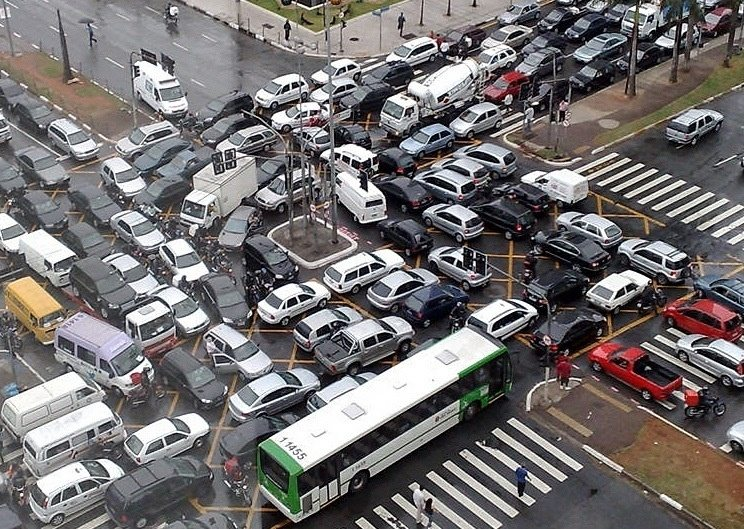
\includegraphics[height=4cm]{deadlock}
      \end{center}
\end{frame}

\begin{frame}
  \frametitle{Une solution pour éviter les deadlocks}
\vFill
  \begin{alertblock}{Composition}
    Des deadlocks peuvent se produire quand plusieurs verrous sont utilisés.
  \end{alertblock}
\vFill
  \begin{block}{Théorème}
    \begin{itemize}
    \item Supposons qu'il y a un ordre sur les verrous $v_1 \le v_2 \le \dots \le v_n$.
    \item Supposons qu'aucun thread ne cherche à obtenir $v$ alors qu'il possède déjà $v'$ avec $v\le v'$.
    \item Alors l'exécution ne comporte pas de deadlock.
    \end{itemize}
  \end{block}

\vFill
  \begin{alertblock}{En TD}
    Utilisez le théorème ci-dessus pour résoudre le problème du dîner des philosophes
  \end{alertblock}
\vFill
\end{frame}

\begin{frame}{Situation de famine}
  \vFill
  \begin{block}{Starvation}
    Situation où un ou  plusieurs threads n'ont \alert{jamais accès}
    à la ressource demandée.
  \end{block}
  \vFill
  \begin{center}
    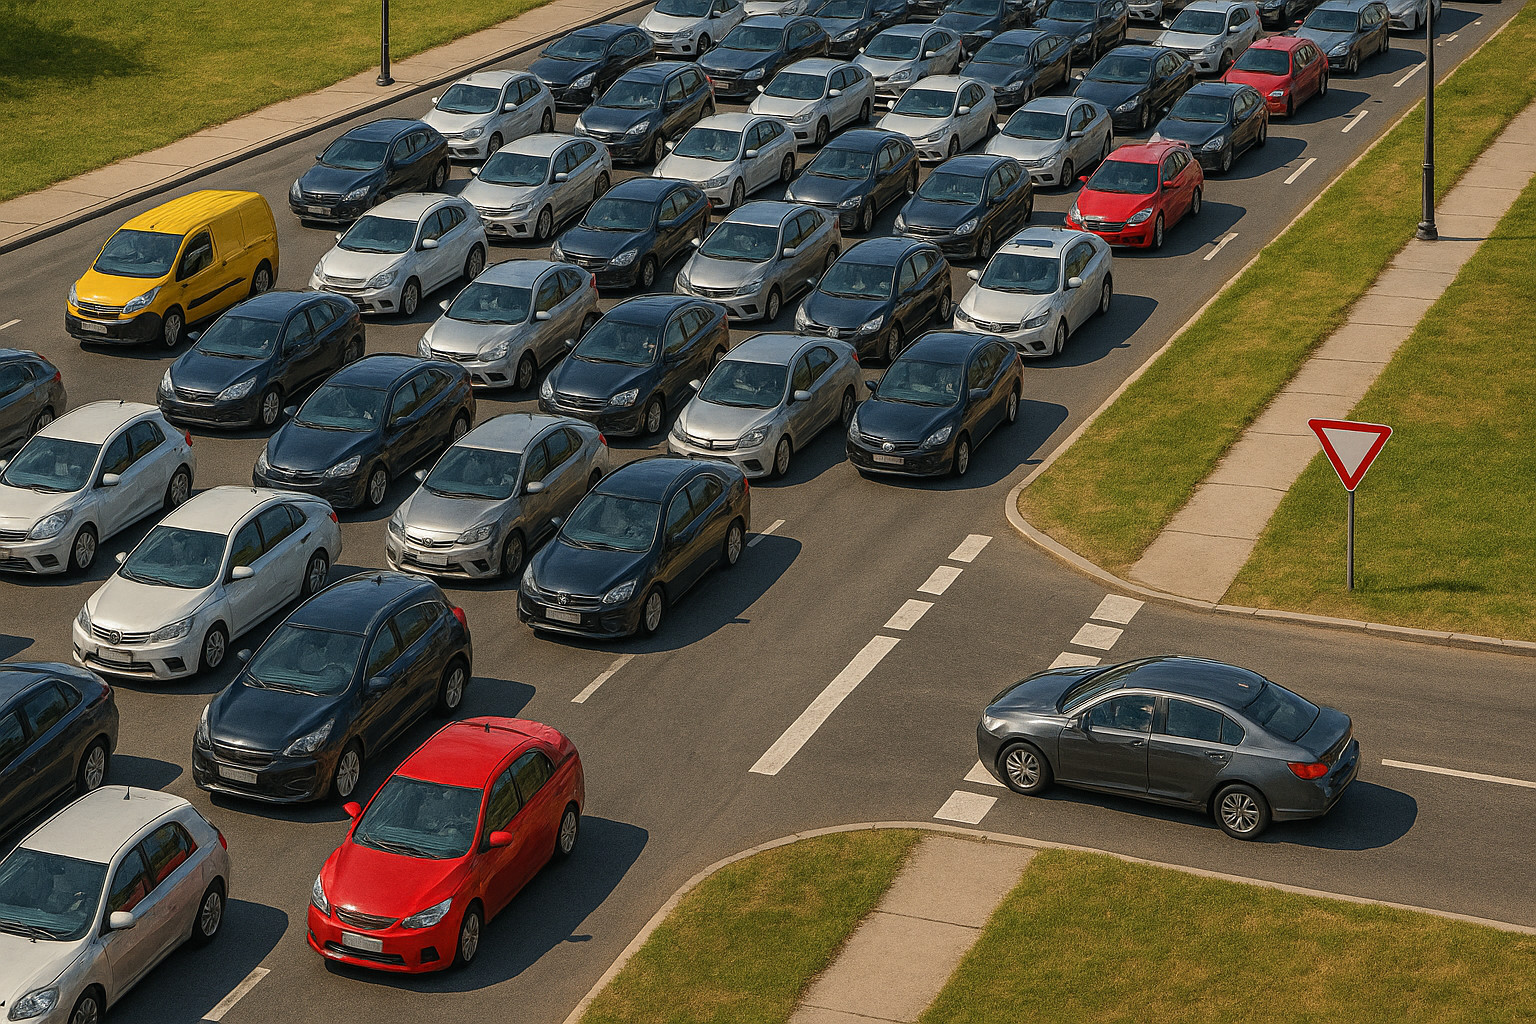
\includegraphics[height=4cm]{starvation}
  \end{center}      
  \vFill
  \begin{alertblock}{En TD}
    Observez les problèmes de famine dans le problème des toilettes unisexes.
  \end{alertblock}
  \vFill
\end{frame}


\subsection{Spécification d'un problème concurrent}
\begin{frame}{Spécification d'un problème réparti}
  \begin{block}{Sûreté (Safety)}
    \begin{itemize}
      \item Rien de mal ne se produit
      $$\forall t. P(t)$$
      \item Thread-safe : fonctionne correctement en multi-thread (très imprécis)
    \end{itemize}
  \end{block}
  \begin{block}{Vivacité (Liveness)}
    \begin{itemize}
      \item Quelque chose de bien finira par se produire
      $$\exists t. P(t)$$
    \end{itemize}
  \end{block}
  \begin{exampleblock}{Exemple : programme qui calcule $\pi$}
    \begin{itemize}
    \item[Sûreté :] \alert{À tout instant}, un préfixe
      de l'écriture décimale de $\pi$ est affiché.
    \item[Vivacité :] Pour tout $n$,
      au moins $n$ chiffres \alert{finiront par} être affichés.
    \end{itemize}
  \end{exampleblock}
\end{frame}

\begin{frame}{Sûreté et vivacité}
  \begin{alertblock}{Infirmez ou confirmez les affirmations suivante}
    \begin{enumerate}
    \item Tous les empires sont des agglomérats de royaumes.
    \item Tous les empires finissent par s'effondrer.
    \end{enumerate}
  \end{alertblock}
  \begin{alertblock}{Propriété de sûreté ou de vivacité ?}
    \begin{enumerate}
    \item Si deux voitures attendent à une intersection, l'une d'elle va finir par passer.
    \item Il n'y aura pas d'accident à l'intersection.
    \item Le feu va passer au vert.
    \item Le feu va passer au vert dans les cinq prochaines minutes.
    \item Seules deux choses sont certaines : la mort et les impôts.
    \end{enumerate}
  \end{alertblock}
\end{frame}

\begin{frame}{Condition de vivacité}

  \begin{block}{Progrès global}
    \alert{Au moins un} thread progresse dans son exécution.
    \begin{itemize}
    \item propriété violée lors d'un interblocage circulaire.
    \end{itemize}
  \end{block}

  \begin{block}{Progrès local}
    \alert{Tous les threads} progressent dans leur exécution.
    \begin{itemize}
    \item propriété violée lors d'une famine.
    \end{itemize}
  \end{block}

\pause
  \begin{alertblock}{Équité (fairness) des verrous}
    \begin{itemize}
    \item Les blocks \lstinline{synchronized}, les verrous \lstinline{ReentrantLock} et les \lstinline{mutex} ne garantissent que le progrès global.
    \item En Java, le constructeur de \lstinline{ReentrantLock} a un argument optionnel :\\
      \lstinline{public ReentrantLock(boolean fair)}
    \end{itemize}
  \end{alertblock}
\end{frame}

\begin{frame}{Caractérisation du progrès global}

  \begin{block}{Deux définitions équivalentes si le nombre de threads est fini}
    Un objet $O$ vérifie le progrès global si, pour toute exécution :
    \begin{enumerate}
    \item Pour tout suffixe de l'exécution, il existe un thread dont toutes les opérations sur $O$ se terminent.
    \item Si l'exécution contient un nombre fini d'opérations sur $O$, elles se terminent toutes.
    \end{enumerate}
  \end{block}

  \begin{exampleblock}{Idée de démonstration : $1 \implies 2$}
    Par récurrence sur le nombre de threads dans l'exécution :
    \begin{enumerate}
    \item S'il n'y a qu'un seul thread, toutes ses opérations se terminent
    \item S'il y a $n+1$ threads, l'un d'entre eux termine toutes ses opérations,
      et on se retrouve avec un suffixe avec $n$ threads. 
    \end{enumerate}
  \end{exampleblock}

  \begin{exampleblock}{Idée de démonstration : $2 \implies 1$}
    Par l'absurde : si aucun thread ne terminait l'une de ses opérations, il y aurait un nombre fini d'opérations dans l'exécution, donc elles termineraient toutes. 
  \end{exampleblock}

\end{frame}


 
\section{Moniteurs}
\mode*
\subsection{Attente et signalement}
\begin{frame}[fragile]{Attente et signalement}
  \begin{tikzpicture}
%    \fill[alertColor!20, rounded corners] (4,6.52) rectangle (6.4,6.82);


    \fill[structure!20, rounded corners] (3.5,3.5) rectangle (8.5,4.15);
    \draw[structure] (11,3.85) node{//$T_{reader}$};

    \draw<2>[alertColor, thick] (3.6,4.03) -- (7.7,4.03);
    \draw<2>[alertColor, thick] (7,4.2) node[above right]{Comment supprimer l'attente active ?};

    \fill[exampleColor!20, rounded corners] (5.1,1.85) rectangle (8.5,2.15);
    \draw[exampleColor] (11,2) node{//$T_{writer}$};
    \draw (5,4.85) node{\begin{minipage}{5cm}\begin{lstlisting}[numbers=none]
class Counter {
  private int value=0;
  public synchronized void increment() {
    ++value;
  }
  public synchronized int get() {
    return value;
  }

  public static void main(String[] args) {
    var counter = new Counter();
    
    new Thread(() -> {
      while(counter.get()==0);
      System.out.println("done");
    }).start();
    
    Thread.sleep(250);
   
    new Thread(counter::increment).start();
  }
}
\end{lstlisting}\end{minipage}};
  \end{tikzpicture}
\end{frame}

\begin{frame}{Sémaphore}
  \begin{center}
    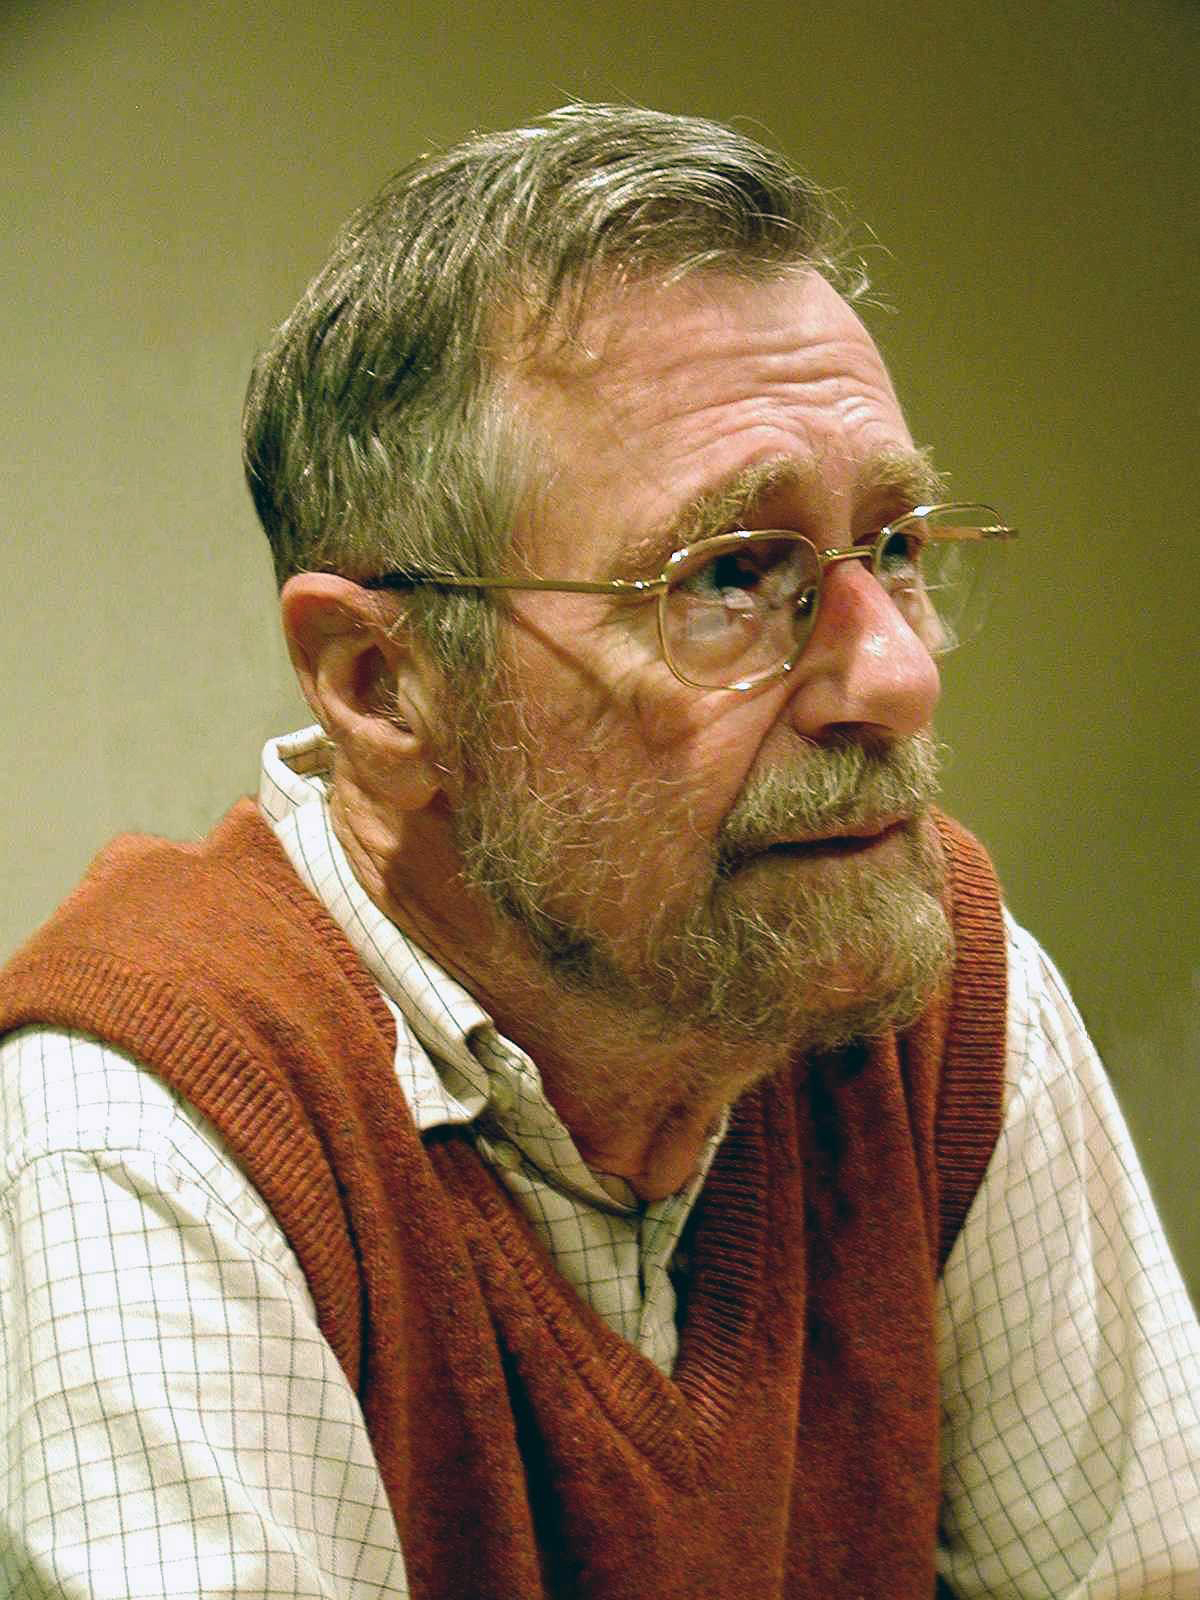
\includegraphics[height=2cm]{Dijkstra}\\
    Edsger W. Dijkstra
  \end{center}
  \vFill
  \begin{block}{Classe \lstinline{java.util.concurrent.Semaphore}}
      \begin{itemize}
      \item \lstinline{new Semaphore(n)}
	\begin{enumerate}
	\item Initialise un sémaphore avec $n$ jetons
	\end{enumerate}
      \item \lstinline{public void acquire() throws InterruptedException}
	\begin{enumerate}
	\item S'il reste un jeton, donner un jeton.
	\item Sinon, attendre qu'un jeton se libère.
	\end{enumerate}
      \item \lstinline{public void release()}
	\begin{enumerate}
	\item Libérer un jeton.
	\end{enumerate}
      \end{itemize}
  \end{block}
  \vFill
  \begin{citing}
  \item[D62] Edsger W. Dijkstra. \textit{Over de sequentialiteit van procesbeschrijvingen (About the sequentiality of process descriptions)} (1962-1963)
  \end{citing}
\end{frame}


\begin{frame}[fragile]{Signalement par sémaphore}
  \begin{tikzpicture}
    \draw (5,4.85) node{\begin{minipage}{5cm}\begin{lstlisting}[numbers=none]
public static void main(String[] args) {
  var semaphore = new Semaphore(0);
  
  new Thread(() -> {
    semaphore.acquire();
    System.out.println("done");
  }).start();
  
  Thread.sleep(250);
 
  new Thread(semaphore::release).start();
}
\end{lstlisting}\end{minipage}};
  \end{tikzpicture}
\end{frame}

\subsection{Notion de moniteur}

\begin{frame}{Moniteur}

  \vFill
  \begin{block}{Construction de synchronisation}
    \begin{itemize}
    \item Un moniteur est un objet encapsulant des données partagées.
    \item Accès aux données partagées en exclusion mutuelle.
    \item Méthodes gardées par des conditions bloquantes (gardes).
    \end{itemize}
  \end{block}

  \vFill
  \hFill
  \begin{minipage}{.4\textwidth}
    \begin{center}
      
\includegraphics[height=3cm]{hansen}\\
      Per Brinch Hansen
    \end{center}
  \end{minipage}
  \hFill
  \begin{minipage}{.5\textwidth}
    \begin{center}
      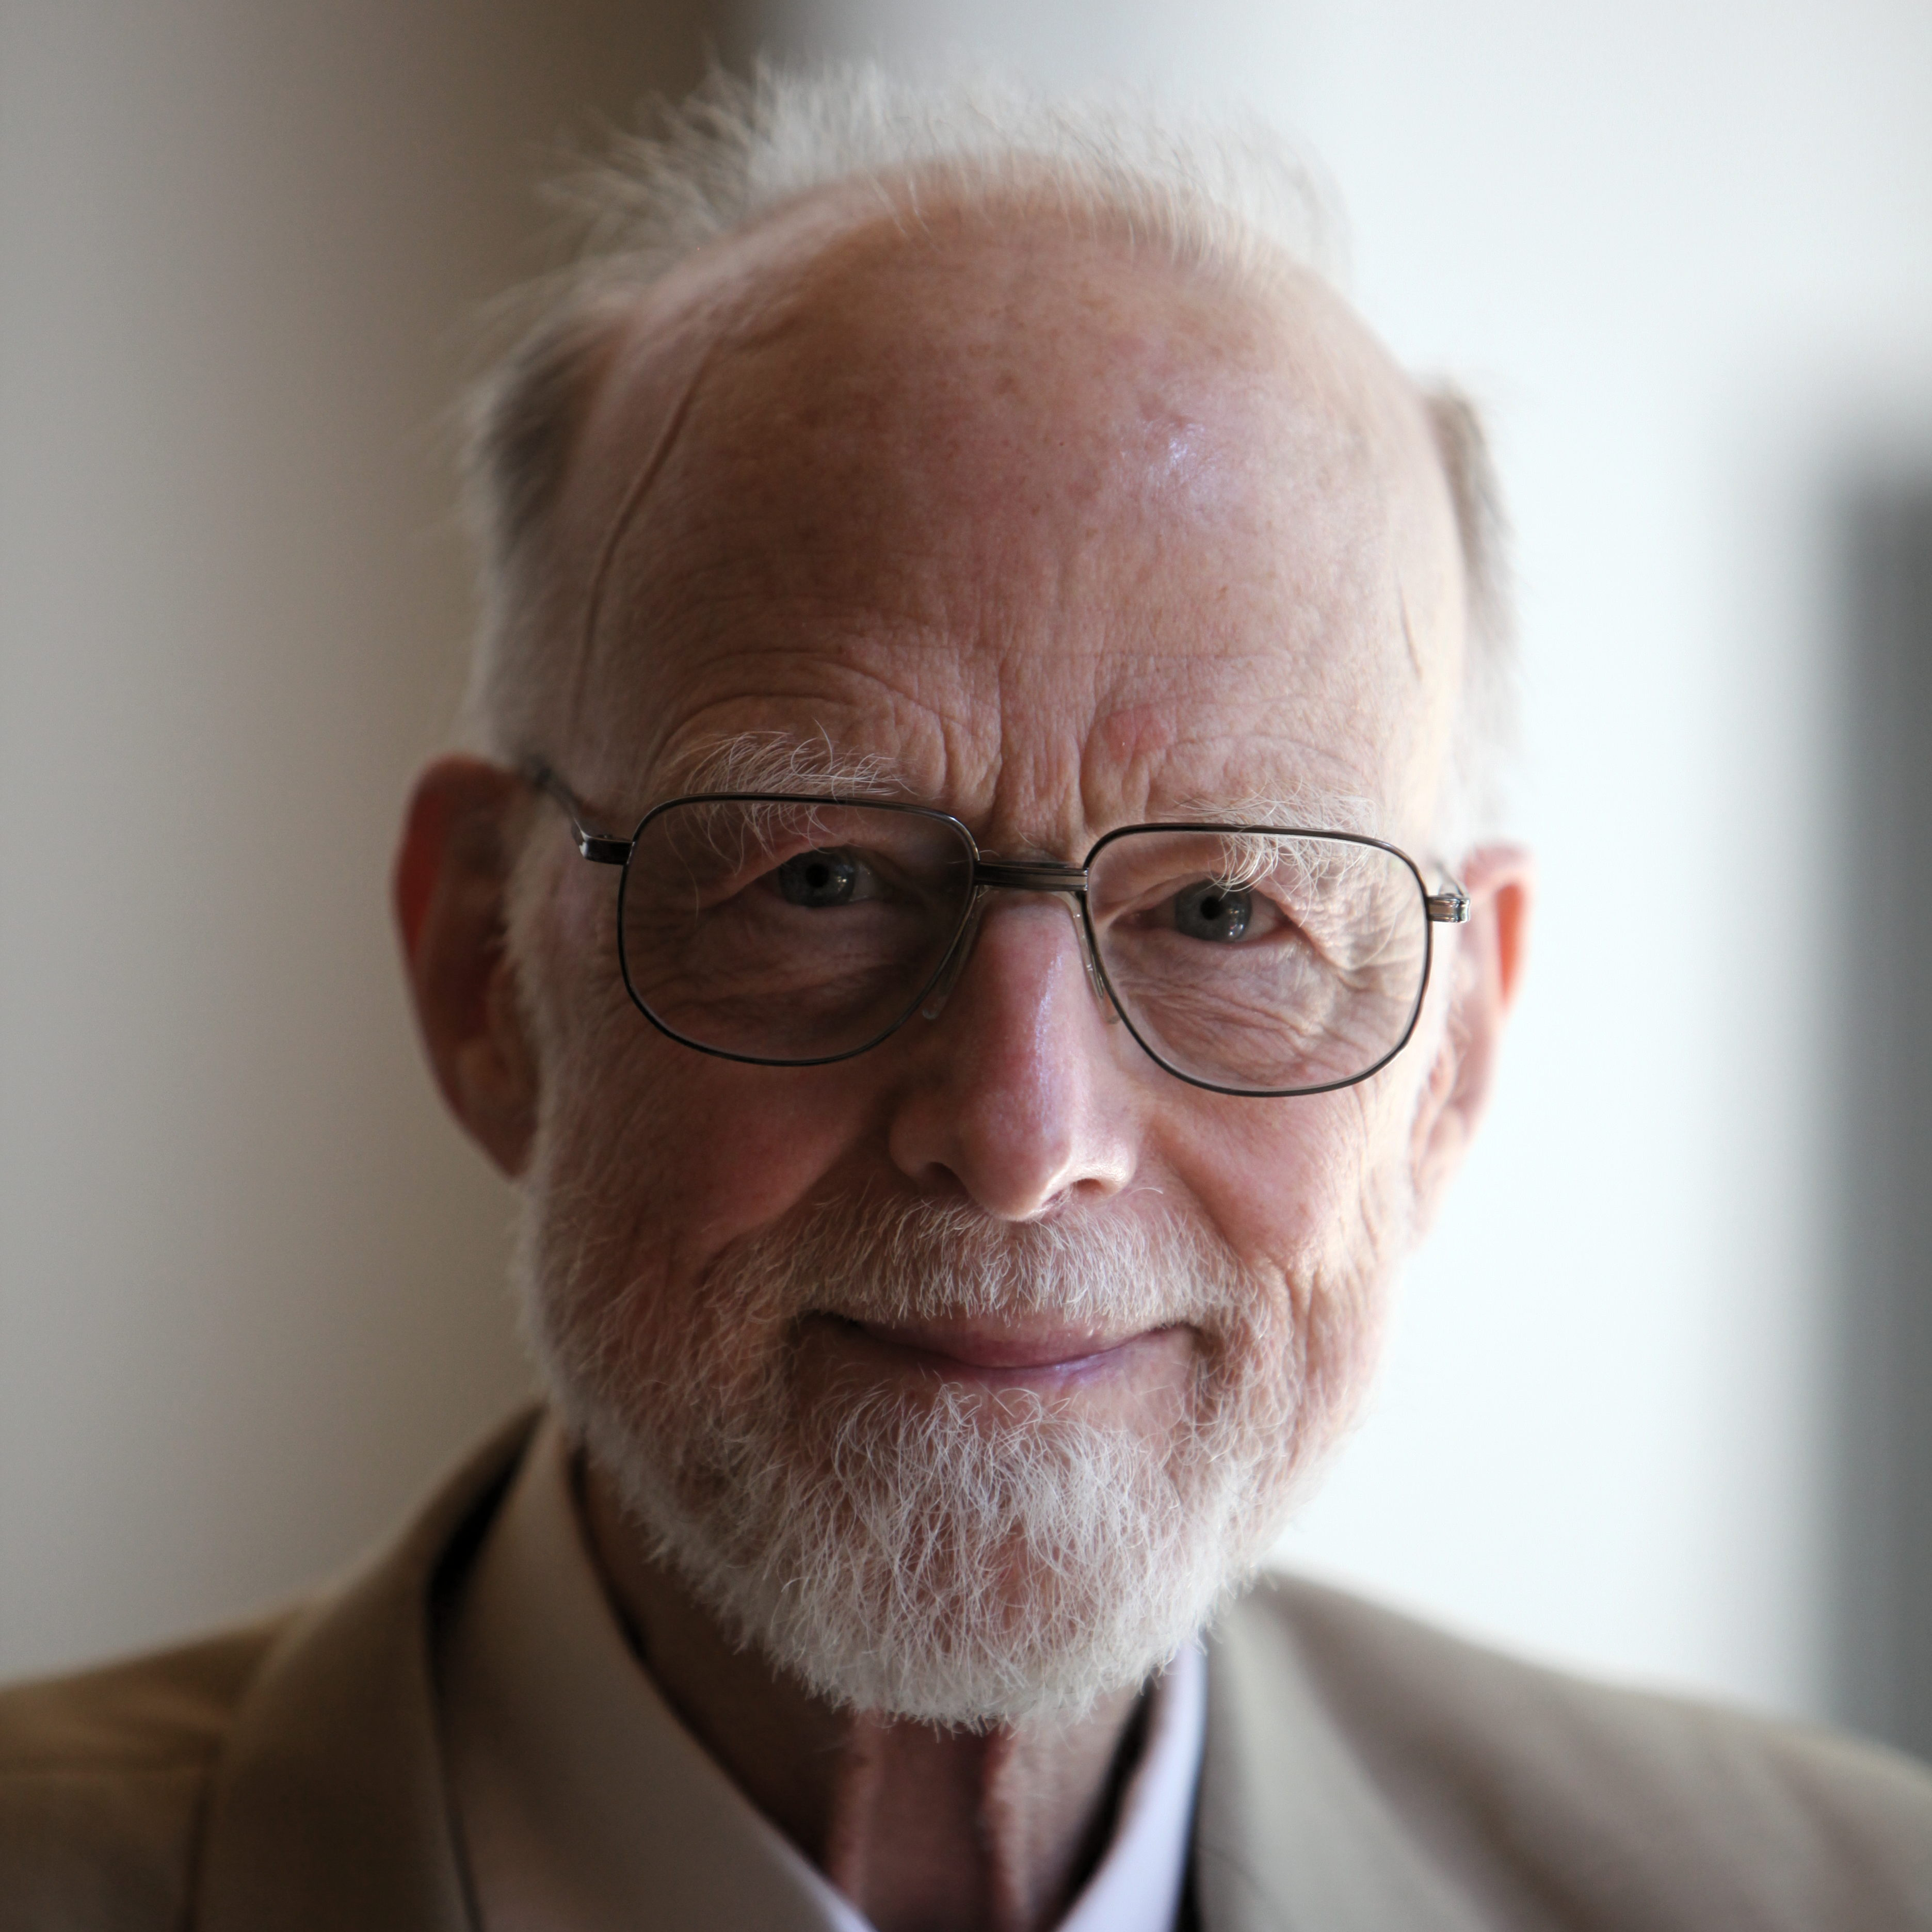
\includegraphics[height=3cm]{hoare}\\
      Tony Hoare
    \end{center}
  \end{minipage}
  \hFill

  \vFill
  \begin{citing}
  \item[] Per Brinch Hansen. \textit{Operating System Principles}. Prentice Hall (1973)
  \item[H74] C. A. R. Hoare. \textit{Monitors: an operating system structuring concept}. CACM (1974)
  \end{citing}
\end{frame}

%%%%%%%%%%%%%%%%%%%%%%%%%%%%%%%%%%%%%%%%%%%%%%%%%%%%%%%%%%%%%%%%%%%%%%%%% 

\begin{frame}{File bloquante}

\vfill
  \begin{exampleblock}{Interface \lstinline{java.util.concurrent.BlockingQueue}}~

\vfill

~\hspace{-5mm}\begin{tabular}{|l|l|l|l|l|}
      \hline
      & Exception & Valeur spéciale & Bloquante & Timeout\\
      \hline
      Insérer & \lstinline+add(e)+ & \lstinline+offer(e)+ & \lstinline+put(e)+ & \lstinline+offer(e, time, unit)+  \\
      \hline
      Supprimer & \lstinline+remove()+ & \lstinline+poll()+ & \lstinline+take()+ & \lstinline+poll(time, unit)+ \\
      \hline
      Regarder & \lstinline+element()+ & \lstinline+peek()+ &  &  \\
      \hline
    \end{tabular}
  \end{exampleblock}

\vfill
\end{frame}

\begin{frame}[fragile]{Le problème des producteurs et des consommateurs}
\vspace{-3mm}
  \begin{tikzpicture}

    \fill[structure!20, rounded corners] (2.8,1.7) rectangle (9.3,4.35);
    \draw[structure] (9.3,3) node[right]{Producteur};
  
    \fill[exampleColor!20, rounded corners] (2.8,5.35) rectangle (9.3,7);
    \draw[exampleColor] (9.3,6.2) node[right]{Consommateur};

    \fill[fill=alertColor!20, rounded corners] (2.8,1.7) rectangle (6,2);
    \fill[fill=alertColor!20, rounded corners] (3.1,3.35) rectangle (6.3,3.65);
    \fill[fill=alertColor!20, rounded corners] (3.1,6.05) rectangle (7,6.35);
    \fill[fill=alertColor!20, rounded corners] (2.4,8.05) rectangle (7.6,8.35);

    \draw (5,4.85) node{\begin{minipage}{5cm}\begin{lstlisting}[numbers=none]
BlockingQueue<Integer> queue
  = new LinkedBlockingQueue<Integer>();

new Thread(() -> {
  int value = 1;
  do {
    value = queue.take();
    System.out.println(value);
  } while(value != 1);
}).start();

new Thread(() -> {
  int value = 17;
  while(value != 1) {
    queue.put(value);
    if(value%2 == 0) value = value/2;
    else value = value*3+1;
    Thread.sleep(500);
  }
  queue.put(value);
}).start();
\end{lstlisting}\end{minipage}};
  \end{tikzpicture}

\vspace{-3mm}
\begin{citing}
\jitem \lstinline{ProducerConsumer.java}
\end{citing}
\end{frame}


%%%%%%%%%%%%%%%%%%%%%%%%%%%%%%%%%%%%%%%%%%%%%%%%%%%%%%%%%%%%%%%%%%%%%%%%% 

\begin{frame} 
  \frametitle{Barrières de synchronisation}

  \begin{exampleblock}{Classe \lstinline+java.util.concurrent.CountDownLatch+}
    \begin{itemize}
    \item \lstinline+public void await() throws InterruptedException+\\
      \begin{itemize}
      \item Se met en attente jusqu'à ce que le compteur atteigne 0
      \end{itemize}
      \medskip
    \item \lstinline+public void countDown()+\\
      \begin{itemize}
      \item Décrémente le compteur
      \end{itemize}
    \end{itemize}
  \end{exampleblock}

  \bigskip
  
  \begin{exampleblock}{Classe \lstinline{java.util.concurrent.CyclicBarrier}}
    \begin{itemize}
    \item\lstinline{public int await() throws InterruptedException, BrokenBarrierExc.}\\
      \begin{itemize}
      \item Se met en attente jusqu'à ce que tous les threads aient rejoint la barrière
      \item Quand tous les threads ont rejoint la barrière, les threads sont réveillés et la barrière est réinitialisée.
      \end{itemize}
      \end{itemize}
  \end{exampleblock}
  
\end{frame}

\subsection{Implémentation}

\begin{frame}[fragile]{Le moniteur universel en Java (\lstinline|java.lang.Object|)}

\vfill    
  \begin{block}{\lstinline|public final void java.lang.Object.wait() throws InterruptedException|}
    \begin{itemize}
    \item Met le thread en attente sur l'objet verrouillé.
    \item Il doit \alert{posséder} le verrou de l'objet sur lequel il se met en attente.
    \item Lorsqu'il entre en attente, il \alert{relâche}  le verrou.
    \end{itemize}
  \end{block}

\vfill    
  \begin{block}{\lstinline|public final void java.lang.Object.notify()|}
    \begin{itemize}
    \item Réveille un des threads en attente sur l'objet verrouillé.
    \item Le thread réveillé doit \alert{acquérir} le verrou.
    \end{itemize}
  \end{block}

\vfill    
  \begin{block}{\lstinline|public final void java.lang.Object.notifyAll()|}
    \begin{itemize}
    \item Pareil mais réveille tous les threads en attente sur l'objet verrouillé.
    \end{itemize}
  \end{block}
\vfill
  \begin{alertblock}{Point vocabulaire}
    \begin{itemize}
    \item Un thread demandant l'accès à un code déjà verrouillé est \alert{bloqué}.
    \item Un  thread qui  est mis  en pause  par l'opération wait est \alert{en attente}.      
    \end{itemize}
  \end{alertblock}
\vfill
\end{frame}


\begin{frame}[fragile]{Implémentation d'un sémaphore}
 
  \begin{lstlisting}
class Semaphore {
  private int counter;
  
  public Semaphore( int counter ) {
    this.counter = counter;
  }
 
  synchronized public void acquire()
  throws InterruptedException {
    while(counter <= 0) wait();
    --counter;
  }
  
  synchronized public void release() {
    ++counter;
    notify();
  }
}
\end{lstlisting}
\end{frame}

\begin{frame}[fragile]{Syntaxes alternatives}
  \begin{block}{En Java : \href{https://docs.oracle.com/javase/7/docs/api/java/util/concurrent/locks/Condition.html}{\lstinline{java.util.concurrent.locks.Condition}}}
\begin{lstlisting}
Lock lock = new ReentrantLock();
Condition condition = lock.newCondition(); 

lock.lock();
condition.signal();
condition.await();
lock.unlock();
\end{lstlisting}
\end{block}
  \begin{block}{En C++ : \href{http://www.cplusplus.com/reference/condition_variable/condition_variable/}{\lstinline{std::condition_variable}}}
\begin{lstlisting}
mutex mtx;
condition_variable condition;

unique_lock<mutex> lock(mtx);
condition.notify_one();
condition.wait(lock);
// unlock on ~unique_lock
\end{lstlisting}
\end{block}
\end{frame}

\mode<all>

 
\section{Implémentation des verrous}
\mode*

\subsection{Réflexions préliminaires}
\begin{frame}[fragile]{Spécification du problème}

\begin{block}{Interface du verrou}
\begin{lstlisting}[numbers=none]
interface Lock {
  void lock() ;
  void unlock() ;
}
\end{lstlisting}
\end{block}

\begin{block}{Spécification logique}
\begin{description}
\item[Exclusion mutuelle : ] Il ne peut jamais y avoir deux threads en section critique en même temps
\item[Starvation-freedom : ] Si un thread cherche à entrer en section critique, il finira par entrer en section critique
\end{description}
\end{block}
\end{frame}


\begin{frame}[fragile]{Un premier essai}
  \begin{tikzpicture}
    \draw (2,8.5) node{
    \begin{tikzpicture}
    \fill[exampleColor!20, rounded corners] (4.25,5.9) rectangle (8.3,6.2);
    \fill[structure!20, rounded corners] (3.1,4.85) rectangle (5.8,5.55);
    \fill[alertColor!20, rounded corners] (3.1,3.85) rectangle (5.8,4.15);

\draw (5,4.85) node{\begin{minipage}{5cm}\begin{lstlisting}[numbers=none]
class NaiveLock1 implements Lock {
  private boolean taken = false;
  public void lock() {
    while(taken);
    taken = true;
  }
  public void unlock() {
    taken = false;
  }
}
\end{lstlisting}\end{minipage}};
  \end{tikzpicture}};

\uncover<1>{
  \draw (4.5,5) node{\begin{minipage}{\textwidth}
  \begin{exampleblock}{Exercice}

  \vspace{2mm}
   Deux threads veulent entrer concurrament en section critique.

  \vspace{2mm}
  \begin{itemize}
  \item Tracer la machine à états du système. 
  \item Montrer que l'exclusion mutuelle n'est pas respectée
  \item Montrer que la starvation-freedom n'est pas respectée
  \end{itemize}
  \end{exampleblock}
  \end{minipage}};
}

\uncover<2->{
  \draw (5,5) node{\begin{tikzpicture}
  \newcommand\tinylst[1]{\scalebox{.5}{\lstinline{#1}}}

   \draw[exampleColor, fill=exampleColor!10, ultra thin, rounded corners] (0,6)    +(-.5,-.35) rectangle +(1.1,.35);
   \draw[structure]    (0,6.2)  node[left]{\tinylst{taken}} node {\tiny=} node[right]{\tinylst{false}};
   \draw               (0,6)    node[left]{\tiny$t1$} node {\tiny:} node[right]{\tinylst{while(taken)}};
   \draw               (0,5.8)  node[left]{\tiny$t2$} node {\tiny:} node[right]{\tinylst{while(taken)}};

   \draw[fill=black!10, ultra thin, rounded corners] (3,6)    +(-.5,-.35) rectangle +(1.1,.35);
   \draw[structure]    (3,6.2)  node[left]{\tinylst{taken}} node {\tiny=} node[right]{\tinylst{false}};
   \draw               (3,6)    node[left]{\tiny$t1$} node {\tiny:} node[right]{\tinylst{taken = true}};
   \draw               (3,5.8)  node[left]{\tiny$t2$} node {\tiny:} node[right]{\tinylst{while(taken)}};

   \draw[fill=black!10, ultra thin, rounded corners] (6,6)    +(-.5,-.35) rectangle +(1.1,.35);
   \draw[structure]    (6,6.2)  node[left]{\tinylst{taken}} node {\tiny=} node[right]{\tinylst{true}};
   \draw               (6,6)    node[left]{\tiny$t1$} node {\tiny:} node[right]{\tiny SC};
   \draw               (6,5.8)  node[left]{\tiny$t2$} node {\tiny:} node[right]{\tinylst{while(taken)}};


   \draw[fill=black!10, ultra thin, rounded corners] (0,4.7)  +(-.5,-.35) rectangle +(1.1,.35);
   \draw[structure]    (0,4.9)  node[left]{\tinylst{taken}} node {\tiny=} node[right]{\tinylst{false}};
   \draw               (0,4.7)  node[left]{\tiny$t1$} node {\tiny:} node[right]{\tinylst{while(taken)}};
   \draw               (0,4.5)  node[left]{\tiny$t2$} node {\tiny:} node[right]{\tinylst{taken = true}};

   \draw[fill=black!10, ultra thin, rounded corners] (3,4.7)  +(-.5,-.35) rectangle +(1.1,.35);
   \draw[structure]    (3,4.9)  node[left]{\tinylst{taken}} node {\tiny=} node[right]{\tinylst{false}};
   \draw               (3,4.7)  node[left]{\tiny$t1$} node {\tiny:} node[right]{\tinylst{taken = true}};
   \draw               (3,4.5)  node[left]{\tiny$t2$} node {\tiny:} node[right]{\tinylst{taken = true}};

   \draw[fill=black!10, ultra thin, rounded corners] (6,4.7)  +(-.5,-.35) rectangle +(1.1,.35);
   \draw[structure]    (6,4.9)  node[left]{\tinylst{taken}} node {\tiny=} node[right]{\tinylst{true}};
   \draw               (6,4.7)  node[left]{\tiny$t1$} node {\tiny:} node[right]{\tiny SC};
   \draw               (6,4.5)  node[left]{\tiny$t2$} node {\tiny:} node[right]{\tinylst{taken = true}};


   \draw[fill=black!10, ultra thin, rounded corners] (0,3.4)    +(-.5,-.35) rectangle +(1.1,.35);
   \draw[structure]    (0,3.6)  node[left]{\tinylst{taken}} node {\tiny=} node[right]{\tinylst{true}};
   \draw               (0,3.4)    node[left]{\tiny$t1$} node {\tiny:} node[right]{\tinylst{while(taken)}};
   \draw               (0,3.2)  node[left]{\tiny$t2$} node {\tiny:} node[right]{\tiny SC};

   \draw[fill=black!10, ultra thin, rounded corners] (3,3.4)    +(-.5,-.35) rectangle +(1.1,.35);
   \draw[structure]    (3,3.6)  node[left]{\tinylst{taken}} node {\tiny=} node[right]{\tinylst{true}};
   \draw               (3,3.4)    node[left]{\tiny$t1$} node {\tiny:} node[right]{\tinylst{taken = true}};
   \draw               (3,3.2)  node[left]{\tiny$t2$} node {\tiny:} node[right]{\tiny SC};

   \draw<3>[alertColor,fill=alertColor!20, ultra thin, rounded corners] (6,3.4)    +(-.5,-.35) rectangle +(1.1,.35);
   \draw<2,4>[fill=black!10, ultra thin, rounded corners] (6,3.4)    +(-.5,-.35) rectangle +(1.1,.35);
   \draw[structure]    (6,3.6)  node[left]{\tinylst{taken}} node {\tiny=} node[right]{\tinylst{true}};
   \draw               (6,3.4)  node[left]{\tiny$t1$} node {\tiny:} node[right]{\tiny SC};
   \draw               (6,3.2)  node[left]{\tiny$t2$} node {\tiny:} node[right]{\tiny SC};

   \draw[-latex]               (-1,6) -- (-.5,6);

   \draw[structure, -latex]    (0.3,5.65) -- (0.3,5.05);
   \draw[structure, -latex]    (0.3,4.35) -- (0.3,3.75);
   \draw<2,4>[structure, -latex]    (3.3,5.65) -- (3.3,5.05);
   \draw<2,4>[structure, -latex]    (3.3,4.35) -- (3.3,3.75);
   \draw<3>[alertColor, -latex]    (3.3,5.65) -- (3.3,5.05);
   \draw<3>[alertColor, -latex]    (3.3,4.35) -- (3.3,3.75);
   \draw[structure, -latex]    (6.3,4.35) -- (6.3,3.75);
   

   \draw[structure, -latex]    (1.1,4.7) -- (2.5,4.7);
   \draw[structure, -latex]    (4.1,4.7) -- (5.5,4.7);
   \draw<2,4>[structure, -latex]    (4.1,3.4) -- (5.5,3.4);
   \draw<3>[alertColor, -latex]    (4.1,3.4) -- (5.5,3.4);

   \draw[structure, -latex]    (1.1,3.3 ) to[out=-20,in=20,distance=15] (1.1,3.5);

     \draw<-3>[structure, -latex]    (6.2,5.65) to[out=-110,in=-80,distance=15] (6.4,5.65);
     \draw<2>[structure, -latex]    (1.1,6.0) -- (2.5,6.0);
     \draw<-3>[structure, -latex]    (4.1,6.0) -- (5.5,6.0);
     \draw<3->[alertColor, -latex]    (1.1,6.0) -- (2.5,6.0);
     \draw<4>[alertColor, -latex]    (4.1,6.0) -- (5.5,6.0);
     \draw<4>[alertColor, -latex]    (6.2,5.65) to[out=-110,in=-80,distance=15] (6.4,5.65);

     \uncover<4>{
       \draw[alertColor, -latex, rounded corners]    (6.3,6.35) -- (6.3,6.6) -- (0.3,6.6) -- (0.3,6.35);
     }

\end{tikzpicture}};
   }
 \end{tikzpicture}
\end{frame}


\begin{frame}[fragile]{Un deuxième essai}

On suppose deux processus, d'identifiants 0 et 1. 

    \begin{tikzpicture}
    \fill[structure!20, rounded corners] (4.25,6.2) rectangle (13.5,6.5);
    \fill[structure!20, rounded corners] (3.1,4.85) rectangle (7.5,5.55);
    \fill[structure!20, rounded corners] (3.1,3.55) rectangle (7.2,3.85);

\draw (5,4.85) node{\begin{minipage}{5cm}\begin{lstlisting}[numbers=none]
class NaiveLock2 implements Lock {
  private boolean[] entering = new boolean[]{false, false};
  public void lock() {
    int i = ThreadID.get();
    entering[i] = true; 
    while(entering[1-i]);
  }
  public void unlock() {
    int i = ThreadID.get();
    entering[i] = false;
  }
}
\end{lstlisting}\end{minipage}};
  \end{tikzpicture}

  \begin{exampleblock}{Exercice}

  \vspace{2mm}
  \begin{itemize}
  \item Cet algorithme respecte-t-il l'exclusion mutuelle ?
  \item Cet algorithme est-il starvation-free ?
  \end{itemize}
  \end{exampleblock}

\end{frame}


\begin{frame}[fragile]{Un troisième essai}

On suppose deux processus, d'identifiants 0 et 1. 

\begin{tikzpicture}
    \fill[exampleColor!20, rounded corners] (4.25,5.9) rectangle (7.4,6.2);
    \fill[exampleColor!20, rounded corners] (3.1,4.85) rectangle (7.1,5.2);
    \fill[exampleColor!20, rounded corners] (3.1,3.55) rectangle (6.0,3.85);

\draw (5,4.7) node{\begin{minipage}{5cm}\begin{lstlisting}[numbers=none]
class NaiveLock3 implements Lock {
  private int priority = 0;
  public void lock() {
    int i = ThreadID.get();
    while(priority != i);
  }
  public void unlock() {
    int i = ThreadID.get();
    priority = 1-i;
  }
}
\end{lstlisting}\end{minipage}};
  \end{tikzpicture}

  \begin{exampleblock}{Exercice}

  \vspace{2mm}
  \begin{itemize}
  \item Cet algorithme respecte-t-il l'exclusion mutuelle ?
  \item Cet algorithme est-il starvation-free ?
  \end{itemize}
  \end{exampleblock}
\end{frame}

\subsection{Algorithme de Peterson}

\begin{frame}[fragile]{Algorithme de Peterson}
On suppose deux processus, d'identifiants 0 et 1. 

\begin{tikzpicture}
    \fill[exampleColor!20, rounded corners] (4.25,5.85) rectangle (7.4,6.15);
    \fill[exampleColor!20, rounded corners] (3.1,4.55) rectangle (6.0,4.82);
    \fill[structure!20, rounded corners] (4.25,6.2) rectangle (13.2,6.5);
    \fill[structure!20, rounded corners] (3.1,4.835) rectangle (7.0,5.15);
    \fill[structure!20, rounded corners] (3.1,2.85) rectangle (7.0,3.15);

\draw (5,4.5) node{\begin{minipage}{5cm}\begin{lstlisting}[numbers=none]
class PetersonLock implements Lock {
  private boolean[] entering = new boolean[]{false, false};
  private int priority = 0;
  public void lock() {
    int i = ThreadID.get();
    entering[i] = true;
    priority = 1-i;
    while(entering[1-i] && priority != i);
  }
  public void unlock() {
    int i = ThreadID.get();
    entering[i] = false;
  }
}
\end{lstlisting}\end{minipage}};
  \end{tikzpicture}

\vspace{-3mm}
  \begin{exampleblock}{Exercice}
  \begin{itemize}
  \item Cet algorithme respecte-t-il l'exclusion mutuelle ?
  \item Cet algorithme est-il starvation-free ?
  \end{itemize}
  \end{exampleblock}

  \vspace{-1mm}
  \begin{citing}
  \item Gary L. Peterson. \textit{Myths About the Mutual Exclusion Problem.} IPL (1981)
  \jitem \lstinline{cm5/PetersonLock.java}
  \end{citing}
\end{frame}



\subsection{Algorithme de la Boulangerie de Lamport}

\begin{frame}[fragile]{Algorithme simplifié}

  \scalebox{.9}{
    \begin{tikzpicture}

      \draw (10.8,0) node{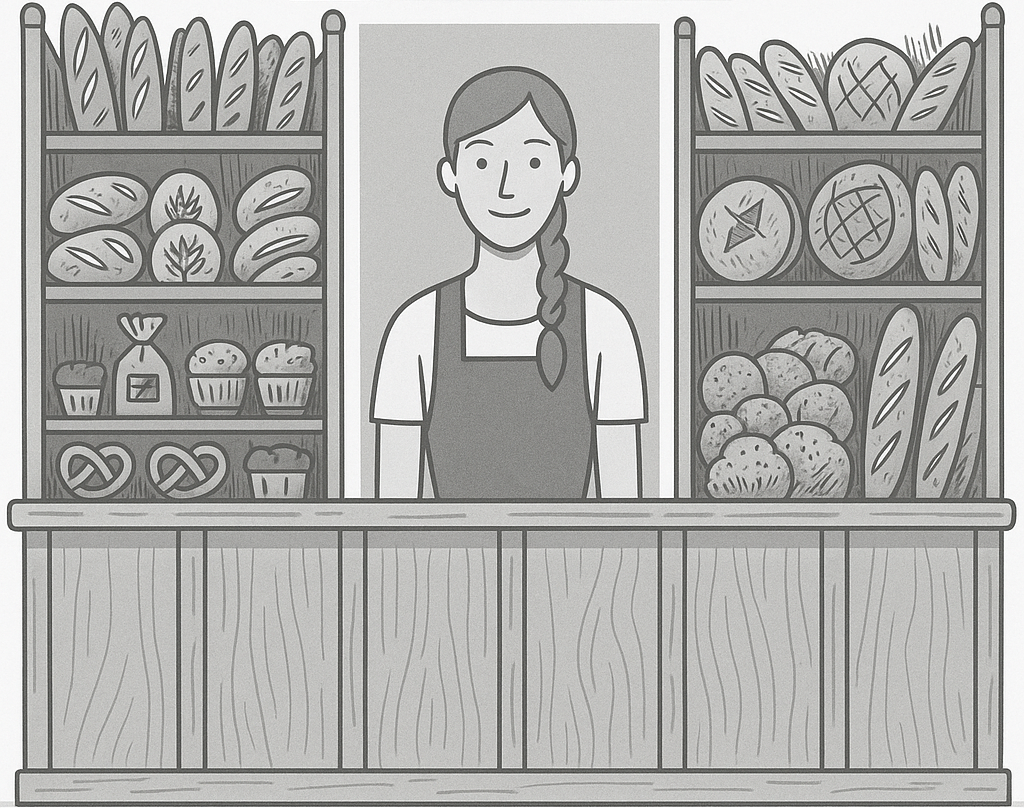
\includegraphics[height=3.3cm]{bakery}};

    \fill<2>[rounded corners, structure!20]       (0,6.6) rectangle (3.8,7.05);
    \fill<2>[rounded corners, structure!20]       (0,2.65) rectangle (2.55,3.1);

    \fill<3>[rounded corners, structure!20] (0,5.5)  rectangle (2.4,5.95);
    \fill<4>[rounded corners, structure!20] (0,4.35) rectangle (7.3,5.5);
    \fill<5>[rounded corners, structure!20] (0,3.7)  rectangle (5.5,4.4);
    
    \draw<2>   (10.8,5) node{
\includegraphics[height=2.5cm]{frenchieBleu}};
    \draw<4>   (1,0)    node{
\includegraphics[height=2.5cm]{frenchieDroit}};
    \draw<2-4> (3.2,0)  node{
\includegraphics[height=2.5cm]{frenchieRouge}};
    \draw<2-4> (5.4,0)  node{
\includegraphics[height=2.5cm]{frenchieVert}};
    \draw<3>   (7.6,0)  node{
\includegraphics[height=2.5cm]{frenchieBleu}};
    \draw<5>   (7.5,0)  node{
\includegraphics[height=2.5cm]{frenchieDroit}};

    \draw<2>  [structure]    (10.7,4.7) node{\Large $\infty$};
    \draw<4>  [structure]    (1.1,-.3)  node{\Large $3$};
    \draw<2-4>[alertColor]   (3.3,-.3)  node{\Large $2$};
    \draw<2-4>[exampleColor] (5.5,-.3)  node{\Large $1$};
    \draw<3>  [structure]    (7.5,-.3)  node{\Large $0$};
    \draw<5>  [structure]    (7.6,-.3)  node{\Large $3$};

    \draw<6> (4,1.4) node{\begin{minipage}{.8\textwidth}
        \begin{block}{Exclusion mutuelle:}
          \vspace{-3mm}
          Supposons $p_i$ et $p_j$ en section critique, avec $\left\langle t_i,i \right\rangle < \left\langle t_j,j \right\rangle$
        \end{block}
    \end{minipage}};

    \draw<6>[->] (0.25,0) node[left]{$p_i$} -- (6.8,0) ;
    \draw<6>[->] (0.25,-.75 ) node[left]{$p_j$} -- (6.8,-.75) ;
    
    \draw<6>[rounded corners, exampleColor, fill=exampleColor!20] (1.75,0)    node{\scriptsize 1: $tickets[i] \leftarrow 0$}   +(-1.3,-.25) rectangle +(1.3,.25);
    \draw<6>[rounded corners, alertColor,   fill=alertColor!20]   (4.9,0)     node{\scriptsize 2: $tickets[j] \rightarrow {<t_j} $}    +(-1.6,-.25) rectangle +(1.6,.25);
    \draw<6>[rounded corners, alertColor,   fill=alertColor!20]   (1.75,-.75) node{\scriptsize 3: $tickets[j] \leftarrow t_j$} +(-1.3,-.25) rectangle +(1.3,.25);
    \draw<6>[rounded corners, exampleColor, fill=exampleColor!20] (4.9,-.75)  node{\scriptsize 4: $tickets[i] \rightarrow \infty$}    +(-1.6,-.25) rectangle +(1.6,.25);
    
    \fill<6>[rounded corners, exampleColor!20] (0,5.5)    rectangle (2.5,5.95);
    \fill<6>[rounded corners, alertColor!20]   (5.2,5.05)  rectangle (7.2,5.5);
    \fill<6>[rounded corners, alertColor!20]   (0,4.35)   rectangle (2.5,4.8);
    \fill<6>[rounded corners, exampleColor!20] (3.45,3.9) rectangle (5.45,4.4);
    
    \draw (5,5) node{\begin{minipage}{\textwidth}
        \begin{algorithm}[H]
        \SetKwFunction{Lock}{lock}
        \SetKwFunction{Unlock}{unlock}
          \SubAlgo{\structure{\textbf{shared variables}}}{
            $tickets[n] \leftarrow [\infty, ..., \infty]$\;
          }
          ~\\
          \SubAlgo{\structure{\textbf{operation}} $\Lock()$}{
            \nl $tickets[i] \leftarrow 0$\;
            \nl \structure{\textbf{let}} $t_i$ \structure{\bf such that} $\displaystyle \left\langle t_i,i \right\rangle > \max_{j : tickets[j] < \infty} \left\langle tickets[j], j\right\rangle$\;
            \nl $tickets[i] \leftarrow t_i$\;
            \nl \structure{\textbf{wait until}} $\displaystyle \left\langle t_i,i \right\rangle = \min_j \left\langle tickets[j], j \right\rangle$.
          }
          ~\\
          \SubAlgo{\structure{\textbf{operation}} $\Unlock()$}{
            $tickets[i] \leftarrow \infty$.
          }
        \end{algorithm}
    \end{minipage}};

    \end{tikzpicture}
    
  }
\end{frame}




\begin{frame}[fragile]{Algorithme de Lamport}
\begin{tikzpicture}
    \fill[exampleColor!20, rounded corners] (4.25,5.85) rectangle (8.8,6.15);
    \fill[exampleColor!20, rounded corners] (3.2,4.65) rectangle (8.5,4.95);
    \fill[exampleColor!20, rounded corners] (3.2,2.25) rectangle (6,2.55);
    \fill[exampleColor!20, rounded corners] (3.2,0.45) rectangle (10.2,1.65);
    \fill[exampleColor!20, rounded corners] (6.9,3.75) rectangle (10.5,4.05);
    \fill[structure!20, rounded corners] (4.25,6.2) rectangle (10.2,6.5);
    \fill[structure!20, rounded corners] (3.2,4.95) rectangle (6.5,5.25);
    \fill[structure!20, rounded corners] (3.2,4.35) rectangle (6.5,4.65);
    \fill[structure!20, rounded corners] (4.55,3.75) rectangle (6.5,4.05);

\draw (8,3.3) node[scale=.9]{\begin{minipage}{1.1\textwidth}\begin{lstlisting}[numbers=none]
class BakeryLock implements Lock {
  private boolean[] entering = new boolean[n]; // {false...}
  private int[] priority = new int[n]; // {0...}
  public void lock() {
    int i = ThreadID.get();
    entering[i] = true;
    priority[i] = 1 + max(priority);
    entering[i] = false;
    for(int j = 0; j < n; j++) {
      while(entering[j] || hasPriorityOverI(j));
    }
  }
  public void unlock() {
    int i = ThreadID.get();
    priority[i] = 0;
  }
  private boolean hasPriorityOverI(int j) {
    if(priority[j] == 0) return false;
    if(priority[j] < priority[i]) return true;
    if(priority[j] == priority[i]) return j<i;
    return false;
  }
}
\end{lstlisting}\end{minipage}};
  \end{tikzpicture}

  \vspace{-2mm}
  \begin{citing}
  \item[L74] Leslie Lamport. \textit{A new solution of Dijkstra's concurrent programming problem.} CACM (1974)
  \jitem \lstinline{cm5/BakeryLock.java}
  \end{citing}

\end{frame}

\subsection{Algorithme spin-lock}

\begin{frame}[fragile]{L'algorithme spin-lock}

\begin{tikzpicture}
    \fill[structure!20, rounded corners] (4.25,5.7) rectangle (12.8,6.0);
    \fill[structure!20, rounded corners] (4.25,4.7) rectangle (8.1,5.0);
    \fill[structure!20, rounded corners] (3.1,3.35) rectangle (6.4,3.65);

\draw (5,4.5) node{\begin{minipage}{5cm}\begin{lstlisting}[numbers=none]
class SpinLock {
  private AtomicBoolean taken = new AtomicBoolean(false);

  public void lock() {
    while(taken.getAndSet(true));
  }

  public void unlock() {
    taken.set(false);
  }
}
\end{lstlisting}\end{minipage}};
  \end{tikzpicture}

\begin{block}{L'opération \alert{atomique} test-and-set}
    \vspace{-2mm}
    \begin{minipage}{.3\textwidth}
    \begin{lstlisting}[numbers=none]
getAndSet(T val) {
  T old = get();
  set(val);
  return old;
}
    \end{lstlisting}
    \end{minipage}
    \hfill    
    \begin{minipage}{.5\textwidth}
    \begin{description}
    \item [Java :] \lstinline{T getAndSet(T val)}
    \item [C++ :] \lstinline{T exchange(T val)}
    \end{description}
    \end{minipage}
    \vspace{-2mm}
  \end{block}

  \vFill
  \begin{citing}
  \item[D62] Edsger W. Dijkstra. \textit{Over de sequentialiteit van procesbeschrijvingen (About the sequentiality of process descriptions)} (1962-1963)
  \jitem \lstinline{cm5/SpinLock.java}
  \end{citing}
\end{frame}


\mode<all>



 
\section{Cohérence des données partagées}
\subsection{Registres atomiques et instructions spéciales}
\mode*

\begin{frame}[fragile]{Registres atomiques}
  \vspace{-2mm}
  \begin{exampleblock}{Java}
  \begin{itemize}
    \item Dans le package \lstinline{java.util.concurrent.atomic}
  \begin{itemize}
    \item \lstinline{AtomicInteger}, \lstinline{AtomicLong}, \lstinline{AtomicReference<T>}, ...
  \end{itemize}
  \end{itemize}
  \end{exampleblock}
  \vspace{-2mm}
  \begin{exampleblock}{C++}
  \begin{itemize}
    \item Structure \lstinline{template <class T> struct std::atomic} 
    \item Fonctions de \lstinline{<atomic>}
  \end{itemize}
 \end{exampleblock}
  \begin{alertblock}{Méthodes \lstinline{get()} et \lstinline{set()} (Java) ou \lstinline{load()} et \lstinline{store()} (C++)}
  \begin{itemize}
    \item Lectures et écritures \structure{atomiques}
  \end{itemize}
  \end{alertblock}
  \begin{block}{Méthodes RMW (read-modify-write)}
    \begin{itemize}
    \item test-and-set, fetch-and-add, compare\_and\_swap...
    \item Opérations atomiques matérielles (instructions spéciales)
    \item Permettent la synchronisation non-bloquante
    \end{itemize}
  \end{block}
\end{frame}


\begin{frame}{Structures de données non-bloquante en Java}
  \begin{itemize}
  \item Compteur : \lstinline{java.util.concurrent.atomic.LongAdder}
    \begin{itemize}
    \item \lstinline{void add(long x)} : incrémente
    \item \lstinline{long sum()} : lit
    \item \alert{Attention : cohérence ?}
    \end{itemize}
  \item File : \lstinline{java.util.concurrent.ConcurrentLinkedQueue<E>} :
    \begin{itemize}
    \item \lstinline{void add(E e)} : ajoute en queue
    \item \lstinline{E peek()} : lit la tête
    \item \lstinline{E poll()} : lit et supprime la tête
    \end{itemize}
  \item Liste doublement chaînée : \lstinline{java.util.concurrent.ConcurrentLinkedDeque<E>}
    \begin{itemize}
    \item \lstinline{void addFirst(E e)}, \lstinline{E getFirst()}, \lstinline{E pollFirst()} : accède la tête
    \item \lstinline{void addLast(E e)}, \lstinline{E getLast()}, \lstinline{E pollLast()} : accède la queue
    \end{itemize}
  \item Table de hashage : \lstinline{java.util.concurrent.ConcurrentHashMap<K,V>}
    \begin{itemize}
    \item \lstinline{put(K key, V value)} : ajoute
    \item \lstinline{get(K key)} : lit
    \item \lstinline{remove(K key)} : supprime une clé
    \item \lstinline{putIfAbsent(K key, V value)} : ajoute ou retourne la valeur
    \end{itemize}
  \end{itemize}
  \begin{citing}
  \item Présentation de Scott sur les structures de données non-bloquantes
  \end{citing}
\end{frame}




\begin{frame}[fragile]{Un compteur non-bloquant}
\small
\begin{itemize}
\item Implémentation de \lstinline{AtomicInteger.getAndIncrement} dans l'\href{https://github.com/openjdk-mirror/jdk7u-jdk/blob/master/src/share/classes/java/util/concurrent/atomic/AtomicInteger.java}{OpenJDK 7}
\end{itemize}

\vspace{-3mm}
  \begin{tikzpicture}
    \fill[alertColor!20, rounded corners] (6.7,6.35) rectangle (7.8,6.65);
    \fill[structure!20, rounded corners] (11.4,6.35) rectangle (11.7,6.65);
    \fill[structure!20, rounded corners] (5.5,5.05) rectangle (7.55,5.35);
    \fill[structure!20, rounded corners] (5.15,4.35) rectangle (6.5,4.65);

    \fill[alertColor!20, rounded corners] (6,5.4) rectangle (7.7,5.7);
    \fill[alertColor!20, rounded corners] (4.3,4.7) rectangle (7.7,5);
    
    \draw (5,5.18) node{\begin{minipage}{5cm}\begin{lstlisting}
class Counter {
  private AtomicInteger value = new AtomicInteger(0); 
  public int getAndIncrement() {
    for (;;) {
      int current = value.get();
      int next = current + 1;
      if (value.compareAndSet(current, next))
        return current;
    }
  }
}
\end{lstlisting}\end{minipage}};

\draw (7,1.2) node{\begin{minipage}{\textwidth}
\begin{block}{L'opération \alert{atomique} compare\_and\_swap}
\vspace{-3mm}
    \begin{lstlisting}[numbers=none]
compareAndSet(T expect, T udpade) {
  if (get() == expect) {
    set(update);
    return true;
  }
  return false;
}
    \end{lstlisting}
  \end{block}
\end{minipage}};

\draw (9,.5) node{\begin{minipage}{\textwidth}
    \begin{description}
    \item [Java :] \lstinline{boolean compareAndSet(T expect, T update)}
    \item [C++ :] \lstinline{bool compare_exchange_strong (T& expected, T val)}
    \end{description}
\end{minipage}};

\draw<2>[exampleColor] (9,3.5) node{Sûreté ?~~~~Vivacité ?};


  \end{tikzpicture}
\end{frame}

\mode<all>



\subsection{La linéarisabilité}
\mode*

\begin{frame}[fragile]{La cohérence séquentielle}

\vfill
\begin{center}
   \alert{Quand peut-on dire qu'une implémentation est \alert{correcte} ?}
\end{center}    

\vfill
\begin{block}{Rappels}
  \begin{itemize}
  \item Raisonnements sur les exécutions à base d'\structure{entrelacements}
  \item Nécessite des exécutions \structure{séquentiellement cohérentes}
  \end{itemize}
\end{block}
\vfill

\begin{block}{Exécution séquentiellement cohérente}
  Le résultat observable d'une exécution est le même que celui d'un entrelacement de l'ordre ``happened before''
\end{block}

\pause

\vfill
\begin{block}{Objet partagé séquentiellement cohérent}
  Le résultat observable \alert{des opérations sur l'objet partagé} d'une exécution est le même que celui d'un entrelacement de l'ordre ``happened before''
\end{block}
\vfill

\end{frame}

\begin{frame}[fragile]{Composabilité des critères de cohérence}
    \begin{lstlisting}[numbers=none]
public static void main(String[] args) {    
  var x = new SequentiallyConsistentCounter(0);
  var y = new SequentiallyConsistentCounter(0);
   
  new Thread(() ->
    x.increment();
    System.out.print(y.get());
  ).start();
   
  new Thread(() ->
    y.increment();
    System.out.print(x.get());
  ).start();
}
    \end{lstlisting}

\vspace{-3mm}
\begin{center}
  \color{exampleColor} Quelles sont les sorties possibles ? 
\end{center}
\pause
\begin{block}{Composabilité}
   \begin{itemize}
      \item Si deux objets sont cohérents, leur composition est cohérente 
      \item \alert{La cohérence séquentielle n'est pas composable !}
   \end{itemize}
\end{block}
\end{frame}


\begin{frame}{Linéarisabilité}
  \vFill
  \hFill
  \begin{minipage}{.6\textwidth}
    \begin{center}
      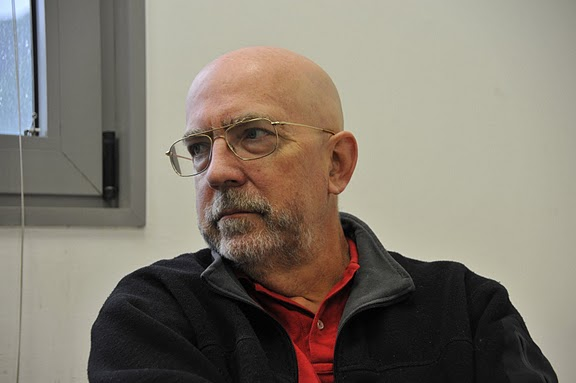
\includegraphics[height=4cm]{Herlihy}\\
      Maurice P. Herlihy
    \end{center}
  \end{minipage}
  \hFill
  \begin{minipage}{.28\textwidth}
    \begin{center}
      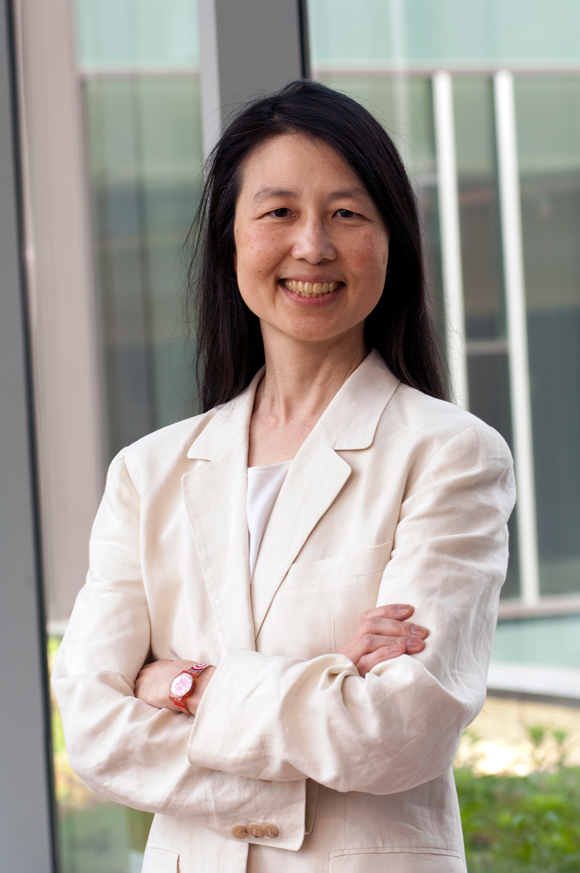
\includegraphics[height=4cm]{Wing}\\
      Jeanette M. Wing
    \end{center}
  \end{minipage}
  \hFill

  \vFill
  \begin{citing}
  \item[L86] Leslie Lamport. \textit{On interprocess communication.} Distributed Computing (1986)
  \item[HW90] Maurice P. Herlihy, Jeanette M. Wing. \textit{Linearizability: A Correctness Condition for Concurrent Objects.} ToPLaS (1990)
  \end{citing}
\end{frame}




\begin{frame}{Linéarisabilité}
  \begin{block}{Définition}
    Un objet partagé est linéarisable si : \\
    le résultat observable des opérations sur l'objet partagé d'une exécution est le même que celui d'un entrelacement de l'ordre ``happened before''
    \alert{tel que, si une opération $e$ se termine avant qu'une autre opération $e'$ ne commence, alors $e$ doit précéder $e'$ dans l'entrelacement}
  \end{block}

\vfill
  \begin{exampleblock}{Exemple}
  \vspace{-3mm}
    \begin{center}
    \scalebox{.7}{
      \begin{tikzpicture}
        \draw[-latex] (0,3) node[left]{$T_1$} -- (10,3);
        \draw[-latex] (0,2) node[left]{$T_2$} -- (10,2);

        \draw[exampleColor, fill=exampleColor!20, rounded corners] (1 , 1.6) rectangle (5 , 2.4);
        \draw[exampleColor, fill=exampleColor!20, rounded corners] (6, 2.6) rectangle (9, 3.4);

        \draw[exampleColor] (3,2) node{$increment()$ };
        \draw[exampleColor] (7.5,3) node{$get()$};
        \end{tikzpicture}
    }
    \end{center}

    Un seul ordre de linéarisation possible : 
    \begin{itemize}
    \item $increment() ;~ get()$
      \begin{itemize}
      \item La lecture doit retourner 1
      \end{itemize}
    \end{itemize}
  \end{exampleblock}

\end{frame}

\begin{frame}{Caractérisation}

  \begin{block}{Point de linéarisation}
    Un objet partagé est linéarisable si, et seulement si : \\
    le résultat observable des opérations sur l'objet partagé d'une exécution est le même que si
    \alert{chaque opération avait lieu en un point atomique
    situé entre son début et sa fin.}
  \end{block}

  \vfill
  \begin{exampleblock}{Exemple}

\begin{center}
    \scalebox{.7}{
      \begin{tikzpicture}
        \draw[exampleColor, -latex] (0,4) node[left]{$counter$} -- (10,4);
        \draw[-latex] (0,3) node[left]{$T_1$} -- (10,3);
        \draw[-latex] (0,2) node[left]{$T_2$} -- (10,2);

        \draw[exampleColor, thick, densely dotted] (3  , 2) -- (3  , 4) node{$\bullet$};
        \draw[exampleColor, thick, densely dotted] (7.5, 3) -- (7.5, 4) node{$\bullet$};

        \draw[exampleColor, fill=exampleColor!20, rounded corners] (1 , 1.6) rectangle (5 , 2.4);
        \draw[exampleColor, fill=exampleColor!20, rounded corners] (6, 2.6) rectangle (9, 3.4);

        \draw[exampleColor] (3,2) node{$increment()$ };
        \draw[exampleColor] (7.5,3) node{$get()$};
        \end{tikzpicture}
    }
    \end{center}
  \end{exampleblock}

\vfill
\small
  \begin{alertblock}{Propriétés}
  \vspace{-2mm}
    \begin{itemize}
      \item La linéarisabilité est composable
      \item La linéarisabilité implique la cohérence séquentielle
      \item Si chaque objet est linéarisable, l'exécution est séquentiellement cohérente
    \end{itemize}
  \end{alertblock}
\end{frame}

\begin{frame}[fragile]{Exemple}
\vspace{-3mm}
\begin{center}
\scalebox{.6}{
      \begin{tikzpicture}
        \draw[white] (-2.5,0.5) rectangle (15,4);

        \draw[structure ,     -latex] (-1,3) node[left]{$T_1$} -- (15,3);
        \draw[exampleColor,   -latex] (-1,2) node[left]{$T_2$} -- (15,2);
        \draw<7> [alertColor, -latex] (-1,1) node[left]{$result$} +(.2,.15) node{$0$} +(0,0) -- (15,1);
        \draw<2-6>[alertColor, -latex] (-1,1) node[left]{$counter$} +(.2,.15) node{$0$} +(0,0) -- (15,1);

        \draw[exampleColor, fill=exampleColor!20, rounded corners] (1 , 1.6) rectangle (5 , 2.4);
        \draw[exampleColor, fill=exampleColor!20, rounded corners] (6 , 1.6) rectangle (13, 2.4);
        \draw[structure, fill=structure!20, rounded corners] (2 , 2.6) rectangle (10, 3.4);
        \draw[structure, fill=structure!20, rounded corners] (11, 2.6) rectangle (14, 3.4);

        \draw<7>[alertColor, fill=alertColor!20, rounded corners] (1.1 , 1.7) rectangle (2.9 , 2.3);
        \draw<7>[alertColor, fill=alertColor!20, rounded corners] (3.1 , 1.7) rectangle (4.9 , 2.3);
        \draw<7>[alertColor, fill=alertColor!20, rounded corners] (6.1 , 1.7) rectangle (12.9, 2.3);
        \draw<7>[alertColor, fill=alertColor!20, rounded corners] (2.1 , 2.7) rectangle (5.4, 3.3);
        \draw<7>[alertColor, fill=alertColor!20, rounded corners] (5.6 , 2.7) rectangle (9.9, 3.3);
        \draw<7>[alertColor, fill=alertColor!20, rounded corners] (11.1, 2.7) rectangle (13.9, 3.3);

        \draw<7>[alertColor] (2   , 2) node{$get()$}; 
        \draw<7>[alertColor] (4   , 2) node{$put(1)$}; 
        \draw<7>[alertColor] (9.5 , 2) node{$get()$}; 
        \draw<7>[alertColor] (4.25, 3) node{$get()$}; 
        \draw<7>[alertColor] (7.75, 3) node{$put(1)$}; 
        \draw<7>[alertColor] (12.5, 3) node{$get()$}; 

        \draw<7>[alertColor, thick, densely dotted] (2   , 1.7) -- (2   , 1) node{$\bullet$} ++(0,.15) node[right]{\footnotesize$0$}; 
        \draw<7>[alertColor, thick, densely dotted] (4   , 1.7) -- (4   , 1) node{$\bullet$} ++(0,.15) node[right]{\footnotesize$1$}; 
        \draw<7>[alertColor, thick, densely dotted] (9.5 , 1.7) -- (9.5 , 1) node{$\bullet$} ++(0,.15) node[right]{\footnotesize$1$}; 
        \draw<7>[alertColor, thick, densely dotted] (3, 2.7)    -- (3, 1)    node{$\bullet$} ++(0,.15) node[right]{\footnotesize$0$}; 
        \draw<7>[alertColor, thick, densely dotted] (7.75, 2.7) -- (7.75, 1) node{$\bullet$} ++(0,.15) node[right]{\footnotesize$1$}; 
        \draw<7>[alertColor, thick, densely dotted] (12.5, 2.7) -- (12.5, 1) node{$\bullet$} ++(0,.15) node[right]{\footnotesize$1$}; 

        \draw<7>[structure] (6,3.65) node{$increment()$ };
        \draw<7>[structure] (12.5,3.65) node{$get()$};
        \draw<7>[exampleColor] (1,1.35) node{$increment()$ };
        \draw<7>[exampleColor] (11,1.35) node{$get()$};

        \draw<-6>[structure] (6,3) node{$increment()$ };
        \draw<1>[structure] (12.5,3) node{$get()$};
        \draw<2>[structure] (12.5,3) node{$get()$ retourne $2$};
        \draw<3>[structure] (12.5,3) node{$get()$ retourne $2$};
        \draw<4>[structure] (12.5,3) node{$get()$ retourne $2$};
        \draw<5>[structure] (12.5,3) node{$get()$ retourne $2$};
        \draw<6>[structure] (12.5,3) node{$get()$ retourne $2$};
        \draw<-6>[exampleColor] (3,2) node{$increment()$ };
        \draw<1>[exampleColor] (9.5,2) node{$get()$};
        \draw<2>[exampleColor] (9.5,2) node{$get()$ retourne $2$};
        \draw<3>[exampleColor] (9.5,2) node{$get()$ retourne $2$};
        \draw<4>[exampleColor] (9.5,2) node{$get()$ retourne $2$};
        \draw<5>[exampleColor] (9.5,2) node{$get()$ retourne $2$};
        \draw<6>[exampleColor] (9.5,2) node{$get()$ retourne $1$};

        \draw<2>[densely dotted, thick, structure]    (4.0  ,2.6) node{$\bullet$} -- (4.0  ,1)    node{$\bullet$};
        \draw<2>[densely dotted, thick, structure]    (11.5 ,2.6) node{$\bullet$} -- (11.5 ,1) node{$\bullet$};
        \draw<2>[densely dotted, thick, exampleColor] (4.5  ,1.6) node{$\bullet$} -- (4.5  ,1)    node{$\bullet$};
        \draw<2>[densely dotted, thick, exampleColor] (12.5 ,1.6) node{$\bullet$} -- (12.5 ,1)  node{$\bullet$};

        \draw<3>[densely dotted, thick, structure]    (4.0  ,2.6) node{$\bullet$} -- (4.0  ,1)    node{$\bullet$};
        \draw<3>[densely dotted, thick, structure]    (13.5 ,2.6) node{$\bullet$} -- (13.5 ,1) node{$\bullet$};
        \draw<3>[densely dotted, thick, exampleColor] (4.5  ,1.6) node{$\bullet$} -- (4.5  ,1)    node{$\bullet$};
        \draw<3>[densely dotted, thick, exampleColor] (9.5  ,1.6) node{$\bullet$} -- (9.5  ,1)  node{$\bullet$};

        \draw<4>[densely dotted, thick, structure]    (5.5  ,2.6) node{$\bullet$} -- (5.5  ,1)    node{$\bullet$};
        \draw<4>[densely dotted, thick, structure]    (11.5 ,2.6) node{$\bullet$} -- (11.5 ,1) node{$\bullet$};
        \draw<4>[densely dotted, thick, exampleColor] (3    ,1.6) node{$\bullet$} -- (3    ,1)    node{$\bullet$};
        \draw<4>[densely dotted, thick, exampleColor] (12.5 ,1.6) node{$\bullet$} -- (12.5  ,1)  node{$\bullet$};

        \draw<5>[densely dotted, thick, structure]    (5.5  ,2.6) node{$\bullet$} -- (5.5  ,1)    node{$\bullet$};
        \draw<5>[densely dotted, thick, structure]    (13.5 ,2.6) node{$\bullet$} -- (13.5 ,1) node{$\bullet$};
        \draw<5>[densely dotted, thick, exampleColor] (3    ,1.6) node{$\bullet$} -- (3    ,1)    node{$\bullet$};
        \draw<5>[densely dotted, thick, exampleColor] (9.5  ,1.6) node{$\bullet$} -- (9.5  ,1)  node{$\bullet$};

        \draw<6>[densely dotted, thick, structure]    (7.5  ,2.6) node{$\bullet$} -- (7.5  ,1)    node{$\bullet$};
        \draw<6>[densely dotted, thick, structure]    (13.5 ,2.6) node{$\bullet$} -- (13.5 ,1) node{$\bullet$};
        \draw<6>[densely dotted, thick, exampleColor] (3    ,1.6) node{$\bullet$} -- (3    ,1)    node{$\bullet$};
        \draw<6>[densely dotted, thick, exampleColor] (6.5  ,1.6) node{$\bullet$} -- (6.5  ,1)  node{$\bullet$};


\end{tikzpicture}
}
\end{center}
\pause
\begin{alertblock}{Linéarisations acceptables}
      \begin{itemize}
      \item $\structure{T_1:increment();}~{\color{exampleColor}T_2:increment();}~\structure{T_1:get();}~{\color{exampleColor}T_2:get();}$
        \begin{itemize}
        \item Les deux lectures retournent 2
        \end{itemize}
        \pause
      \item $\structure{T_1:increment();}~{\color{exampleColor}T_2:increment();}~{\color{exampleColor}T_2:get();}~\structure{T_1:get();}$
        \begin{itemize}
        \item Les deux lectures retournent 2
        \end{itemize}
        \pause
      \item ${\color{exampleColor}T_2:increment();}~\structure{T_1:increment();}~\structure{T_1:get();}~{\color{exampleColor}T_2:get();}$
        \begin{itemize}
        \item Les deux lectures retournent 2
        \end{itemize}
        \pause
      \item ${\color{exampleColor}T_2:increment();}~\structure{T_1:increment();}~{\color{exampleColor}T_2:get();}~\structure{T_1:get();}$
        \begin{itemize}
        \item Les deux lectures retournent 2
        \end{itemize}
        \pause
      \item ${\color{exampleColor}T_2:increment();}~{\color{exampleColor}T_2:get();}~\structure{T_1:increment();}~\structure{T_1:get();}$
        \begin{itemize}
        \item $T_1$ lit $2$ et $T_2$ lit $1$
        \end{itemize}
      \end{itemize}
      \end{alertblock}
%    \end{itemize}

\end{frame}





\begin{frame}{Algorithmes d'incrémentation}
\begin{block}{Algorithme bloquant}
\begin{itemize}
\item Point de linéarisation n'importe où en section critique
\end{itemize}
\centering
\scalebox{.6}{\begin{tikzpicture}
        \draw[exampleColor, fill=exampleColor!20, rounded corners] (0.6,0.6)  rectangle (10.1,1.4);
        \draw[alertColor, fill=alertColor!20, rounded corners] (0.6,-0.4) rectangle (5.8,0.4);
 
        \draw[structure, -latex] (0,2) node[left]{$counter$} +(.2,.15) node{$0$} +(0,0) -- (10.5,2);
        \draw[exampleColor,-latex] (0,1) node[left]{$t1$} -- (10.5,1);
        \draw[alertColor, -latex] (0,0) node[left]{$t2$} -- (10.5,0);
        \draw[structure, -latex] (0,-1   ) node[left]{\scriptsize $value$} +(.15,.12) node{\scriptsize $0$} +(0,0) -- (10.5,-1   );
        \draw[structure, -latex] (0,-1.25) node[left]{\scriptsize $lock$}  +(0,0) -- (10.5,-1.25);
 
        \draw[exampleColor, thick, densely dotted] (7.9 ,1.4) node{$\bullet$} -- (7.9 ,2) node{$\bullet$} ++(0,.15) node[left]{\footnotesize$increment()$} node[right]{\footnotesize$2$}; 
        \draw[alertColor,   thick, densely dotted] (3.6 ,0.4) node{$\bullet$} -- (3.6 ,2) node{$\bullet$} ++(0,.15) node[left]{\footnotesize$increment()$} node[right]{\footnotesize$1$}; 
 
        \draw[alertColor,   ultra thick] (1.2 ,-1.25) -- (5.0 ,-1.25) ; 
        \draw[exampleColor, ultra thick] (5.75 ,-1.25) -- (9.3 ,-1.25) ; 
 
 
        \draw[structure, thick, densely dotted] (5.75 ,1) -- (5.75 ,-1.25) node{$\bullet$} +(.15,.12) ; 
        \draw[structure, thick, densely dotted] (6.7 ,1) -- (6.7 ,-1   ) node{$\bullet$} +(.15,.12) node{\scriptsize $1$}; 
        \draw[structure, thick, densely dotted] (7.9 ,1) -- (7.9 ,-1   ) node{$\bullet$} +(.15,.12) node{\scriptsize $2$}; 
        \draw[structure, thick, densely dotted] (9.3 ,1) -- (9.3 ,-1.25) node{$\bullet$} +(.15,.12) ; 
        \draw[structure, thick, densely dotted] (1.2 ,0) -- (1.2 ,-1.25) node{$\bullet$} +(.15,.12) ; 
        \draw[structure, thick, densely dotted] (2.4 ,0) -- (2.4 ,-1   ) node{$\bullet$} +(.15,.12) node{\scriptsize $0$}; 
        \draw[structure, thick, densely dotted] (3.6 ,0) -- (3.6 ,-1   ) node{$\bullet$} +(.15,.12) node{\scriptsize $1$}; 
        \draw[structure, thick, densely dotted] (5.0 ,0) -- (5.0 ,-1.25) node{$\bullet$} +(.15,.12) ; 
 
 
        \draw[structure, fill=structure!20, rounded corners] (3.0 ,1)  +(-2.3,-0.3) rectangle +(3.0,0.3) +(0,0) node{$lock()$};
        \draw[structure, fill=structure!20, rounded corners] (6.7 ,1)  +(-0.5,-0.3) rectangle +(0.5,0.3) +(0,0) node{$get()$};
        \draw[structure, fill=structure!20, rounded corners] (7.9 ,1)  +(-0.5,-0.3) rectangle +(0.5,0.3) +(0,0) node{$set(2)$};
        \draw[structure, fill=structure!20, rounded corners] (9.3 ,1)  +(-0.7,-0.3) rectangle +(0.7,0.3) +(0,0) node{$unlock()$};
        \draw[structure, fill=structure!20, rounded corners] (1.2 ,0)  +(-0.5,-0.3) rectangle +(0.5,0.3) +(0,0) node{$lock()$};
        \draw[structure, fill=structure!20, rounded corners] (2.4 ,0)  +(-0.5,-0.3) rectangle +(0.5,0.3) +(0,0) node{$get()$};
        \draw[structure, fill=structure!20, rounded corners] (3.6 ,0)  +(-0.5,-0.3) rectangle +(0.5,0.3) +(0,0) node{$set(1)$};
        \draw[structure, fill=structure!20, rounded corners] (5.0 ,0)  +(-0.7,-0.3) rectangle +(0.7,0.3) +(0,0) node{$unlock()$};
 
 
        \end{tikzpicture}}
        \end{block}
\begin{block}{Algorithme non-bloquant}
\begin{itemize}
\item Point de linéarisation sur la dernière instruction \lstinline{compareAndSet} 
\end{itemize}
\centering
   \scalebox{.6}{\begin{tikzpicture}
        \draw[exampleColor, fill=exampleColor!20, rounded corners] (0.6,0.6)  rectangle (10.1,1.4);
        \draw[alertColor, fill=alertColor!20, rounded corners] (0.6,-0.4) rectangle (5.8,0.4);
 
        \draw[structure, -latex] (0,2) node[left]{$counter$} +(.2,.15) node{$0$} +(0,0) -- (10.5,2);
        \draw[exampleColor,-latex] (0,1) node[left]{$t1$} -- (10.5,1);
        \draw[alertColor, -latex] (0,0) node[left]{$t2$} -- (10.5,0);
        \draw[structure, -latex] (0,-1   ) node[left]{\scriptsize $value$} +(.15,.12) node{\scriptsize $0$} +(0,0) -- (10.5,-1   );
 
        \draw[exampleColor, thick, densely dotted] (8.0 ,1.4) node{$\bullet$} -- (8.0 ,2) node{$\bullet$} ++(0,.15) node[left]{\footnotesize$increment()$} node[right]{\footnotesize$2$}; 
        \draw[alertColor,   thick, densely dotted] (4.0 ,0.4) node{$\bullet$} -- (4.0 ,2) node{$\bullet$} ++(0,.15) node[left]{\footnotesize$increment()$} node[right]{\footnotesize$1$};  
 
        \draw[structure, thick, densely dotted] (8.0 ,1) -- (8.0 ,-1) node{$\bullet$} +(.15,.12) node{\scriptsize $2$}; 
        \draw[structure, thick, densely dotted] (4.0 ,0) -- (4.0 ,-1) node{$\bullet$} +(.15,.12) node{\scriptsize $1$}; 
        \draw[structure, thick, densely dotted] (3.0 ,1) -- (3.0 ,-1) node{$\bullet$};
        \draw[structure, thick, densely dotted] (5.0 ,1) -- (5.0 ,-1) node{$\bullet$};
        \draw[structure, thick, densely dotted] (6.5 ,1) -- (6.5 ,-1) node{$\bullet$};
        \draw[structure, thick, densely dotted] (2.0 ,0) -- (2.0 ,-1) node{$\bullet$};


        \draw[structure, fill=structure!20, rounded corners] (3.0 ,1)  +(-0.50,-0.3) rectangle +(0.50,0.3) +(0,0) node{$get()$};
        \draw[structure, fill=structure!20, rounded corners] (5.0 ,1)  +(-0.75,-0.3) rectangle +(0.75,0.3) +(0,0) node{$cas(0, 1)$};
        \draw[structure, fill=structure!20, rounded corners] (6.5 ,1)  +(-0.50,-0.3) rectangle +(0.50,0.3) +(0,0) node{$get()$};
        \draw[structure, fill=structure!20, rounded corners] (8.0 ,1)  +(-0.75,-0.3) rectangle +(0.75,0.3) +(0,0) node{$cas(1, 2)$};
        \draw[structure, fill=structure!20, rounded corners] (2.0 ,0)  +(-0.50,-0.3) rectangle +(0.50,0.3) +(0,0) node{$get()$};
        \draw[structure, fill=structure!20, rounded corners] (4.0 ,0)  +(-0.75,-0.3) rectangle +(0.75,0.3) +(0,0) node{$cas(0, 1)$};
 
        \end{tikzpicture}}
        \end{block}
\end{frame}



\mode<all>



\subsection{Modèles de mémoire}
\mode*

\begin{frame}[fragile]{Que fait ce programme ?}
  \begin{tikzpicture}
    \fill[alertColor!20, rounded corners] (4,6.52) rectangle (6.4,6.82);
    \draw[alertColor, thick] (4.1,6.67) -- (6.3,6.67);

    \fill[structure!20, rounded corners] (3.5,3.5) rectangle (8.5,4.15);
    \draw[structure] (11,3.85) node{//$T_{reader}$};

    \fill[exampleColor!20, rounded corners] (5.1,1.85) rectangle (8.5,2.15);
    \draw[exampleColor] (11,2) node{//$T_{writer}$};
    \draw (5,4.85) node{\begin{minipage}{5cm}\begin{lstlisting}[numbers=none]
class Counter {
  private int value=0;
  public synchronized void increment() {
    ++value;
  }
  public synchronized int get() {
    return value;
  }

  public static void main(String[] args) {
    var counter = new Counter();
    
    new Thread(() -> {
      while(counter.get()==0);
      System.out.println("done");
    }).start();
    
    Thread.sleep(250);
   
    new Thread(counter::increment).start();
  }
}
\end{lstlisting}\end{minipage}};
  \end{tikzpicture}
  
  \vspace{-5mm}
\begin{citing}
\jitem \lstinline{tp1/Volatile.java}
\end{citing}
\end{frame}

\begin{frame}[fragile]{Quels affichages sont possibles ?}
  \vspace{-3mm}
  \begin{tikzpicture}
    \fill[structure!20, rounded corners] (4,5.85) rectangle (6.5,6.5);
    \fill[structure!20, rounded corners] (3.5,4.85) rectangle (8.3,5.2);
    \fill[structure!20, rounded corners] (3.5,3.85) rectangle (9.9,4.2);
    \draw (5,4.85) node{\begin{minipage}{5cm}\begin{lstlisting}[numbers=none]
class Optimizations {
  static int sum = 0;
  static int i = 0;
  public static void main(String args[]) {
    new Thread(() -> {
      for(i=1; i<2; i++) sum+=i;
    }).start();
    new Thread(() -> {
      if(sum != 0) System.out.println(i);
    }).start();
  }
}
\end{lstlisting}\end{minipage}};
  \end{tikzpicture}
  \pause
    \vspace{-2mm}
  \begin{block}{Compilateur et JVM : respect de la sémantique séquentielle}
    \vspace{-3mm}
    \begin{minipage}{.35\textwidth}
    \begin{lstlisting}[numbers=none]
for(i=1; i<2; i++)
  sum+=i;

\end{lstlisting}
    \end{minipage}
    \pause
    \hspace{\fill}
    \begin{minipage}{.2\textwidth}
    \begin{lstlisting}[numbers=none]
i=1;
sum=1;
i=2;
    \end{lstlisting}
    \end{minipage}
    \hspace{\fill}
    \pause
    \begin{minipage}{.2\textwidth}
    \begin{lstlisting}[numbers=none]
      
sum=1;
i=2;
    \end{lstlisting}
    \end{minipage}
  \end{block}

    \vspace{-2mm}
\pause
  \begin{exampleblock}{Mot-clé \lstinline{volatile int x;}}
    \begin{itemize}
    \item Pas d'optimisation qui change la position d'une opération sur $x$
    \end{itemize}
  \end{exampleblock}
\end{frame}

\begin{frame}[fragile]{Cohérence de cache}
  \begin{block}{Architectures UMA (Uniform Memory Access)}
    \begin{center}
      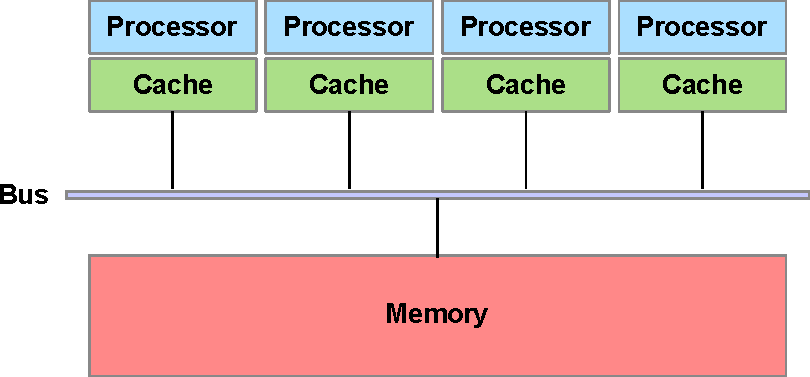
\includegraphics[height=2cm]{uma}
    \end{center}
  \end{block}
  \begin{exampleblock}{Mot-clé \lstinline{volatile int x;} (depuis Java 5)}
    \begin{itemize}
    \item Tout le cache est invalidé \structure{avant chaque lecture}  de $x$
    \item Tout le cache est invalidé \structure{après chaque écriture} de $x$
    \item Le cache n'est pas invalidé \structure{pendant} une lecture ou écriture de $x$ $^\star$
    \end{itemize}
  \end{exampleblock}
  \begin{alertblock}{Attention}
    \begin{itemize}
    \item Une invalidation de cache est très inefficace !
    \end{itemize}
  \end{alertblock}

\vfill

\fontsize{4}{4}\selectfont{ $^\star$ \href{https://docs.oracle.com/javase/specs/jls/se7/html/jls-17.html#jls-17.7}{(§17.7)} \it Implementations of the Java Virtual Machine are \alert{encouraged} to avoid splitting 64-bit values where possible. Programmers are encouraged to declare shared 64-bit values as volatile or synchronize their programs correctly to avoid possible complications.}

\end{frame}


\begin{frame}{Échelles de temps}
   \begin{center}
      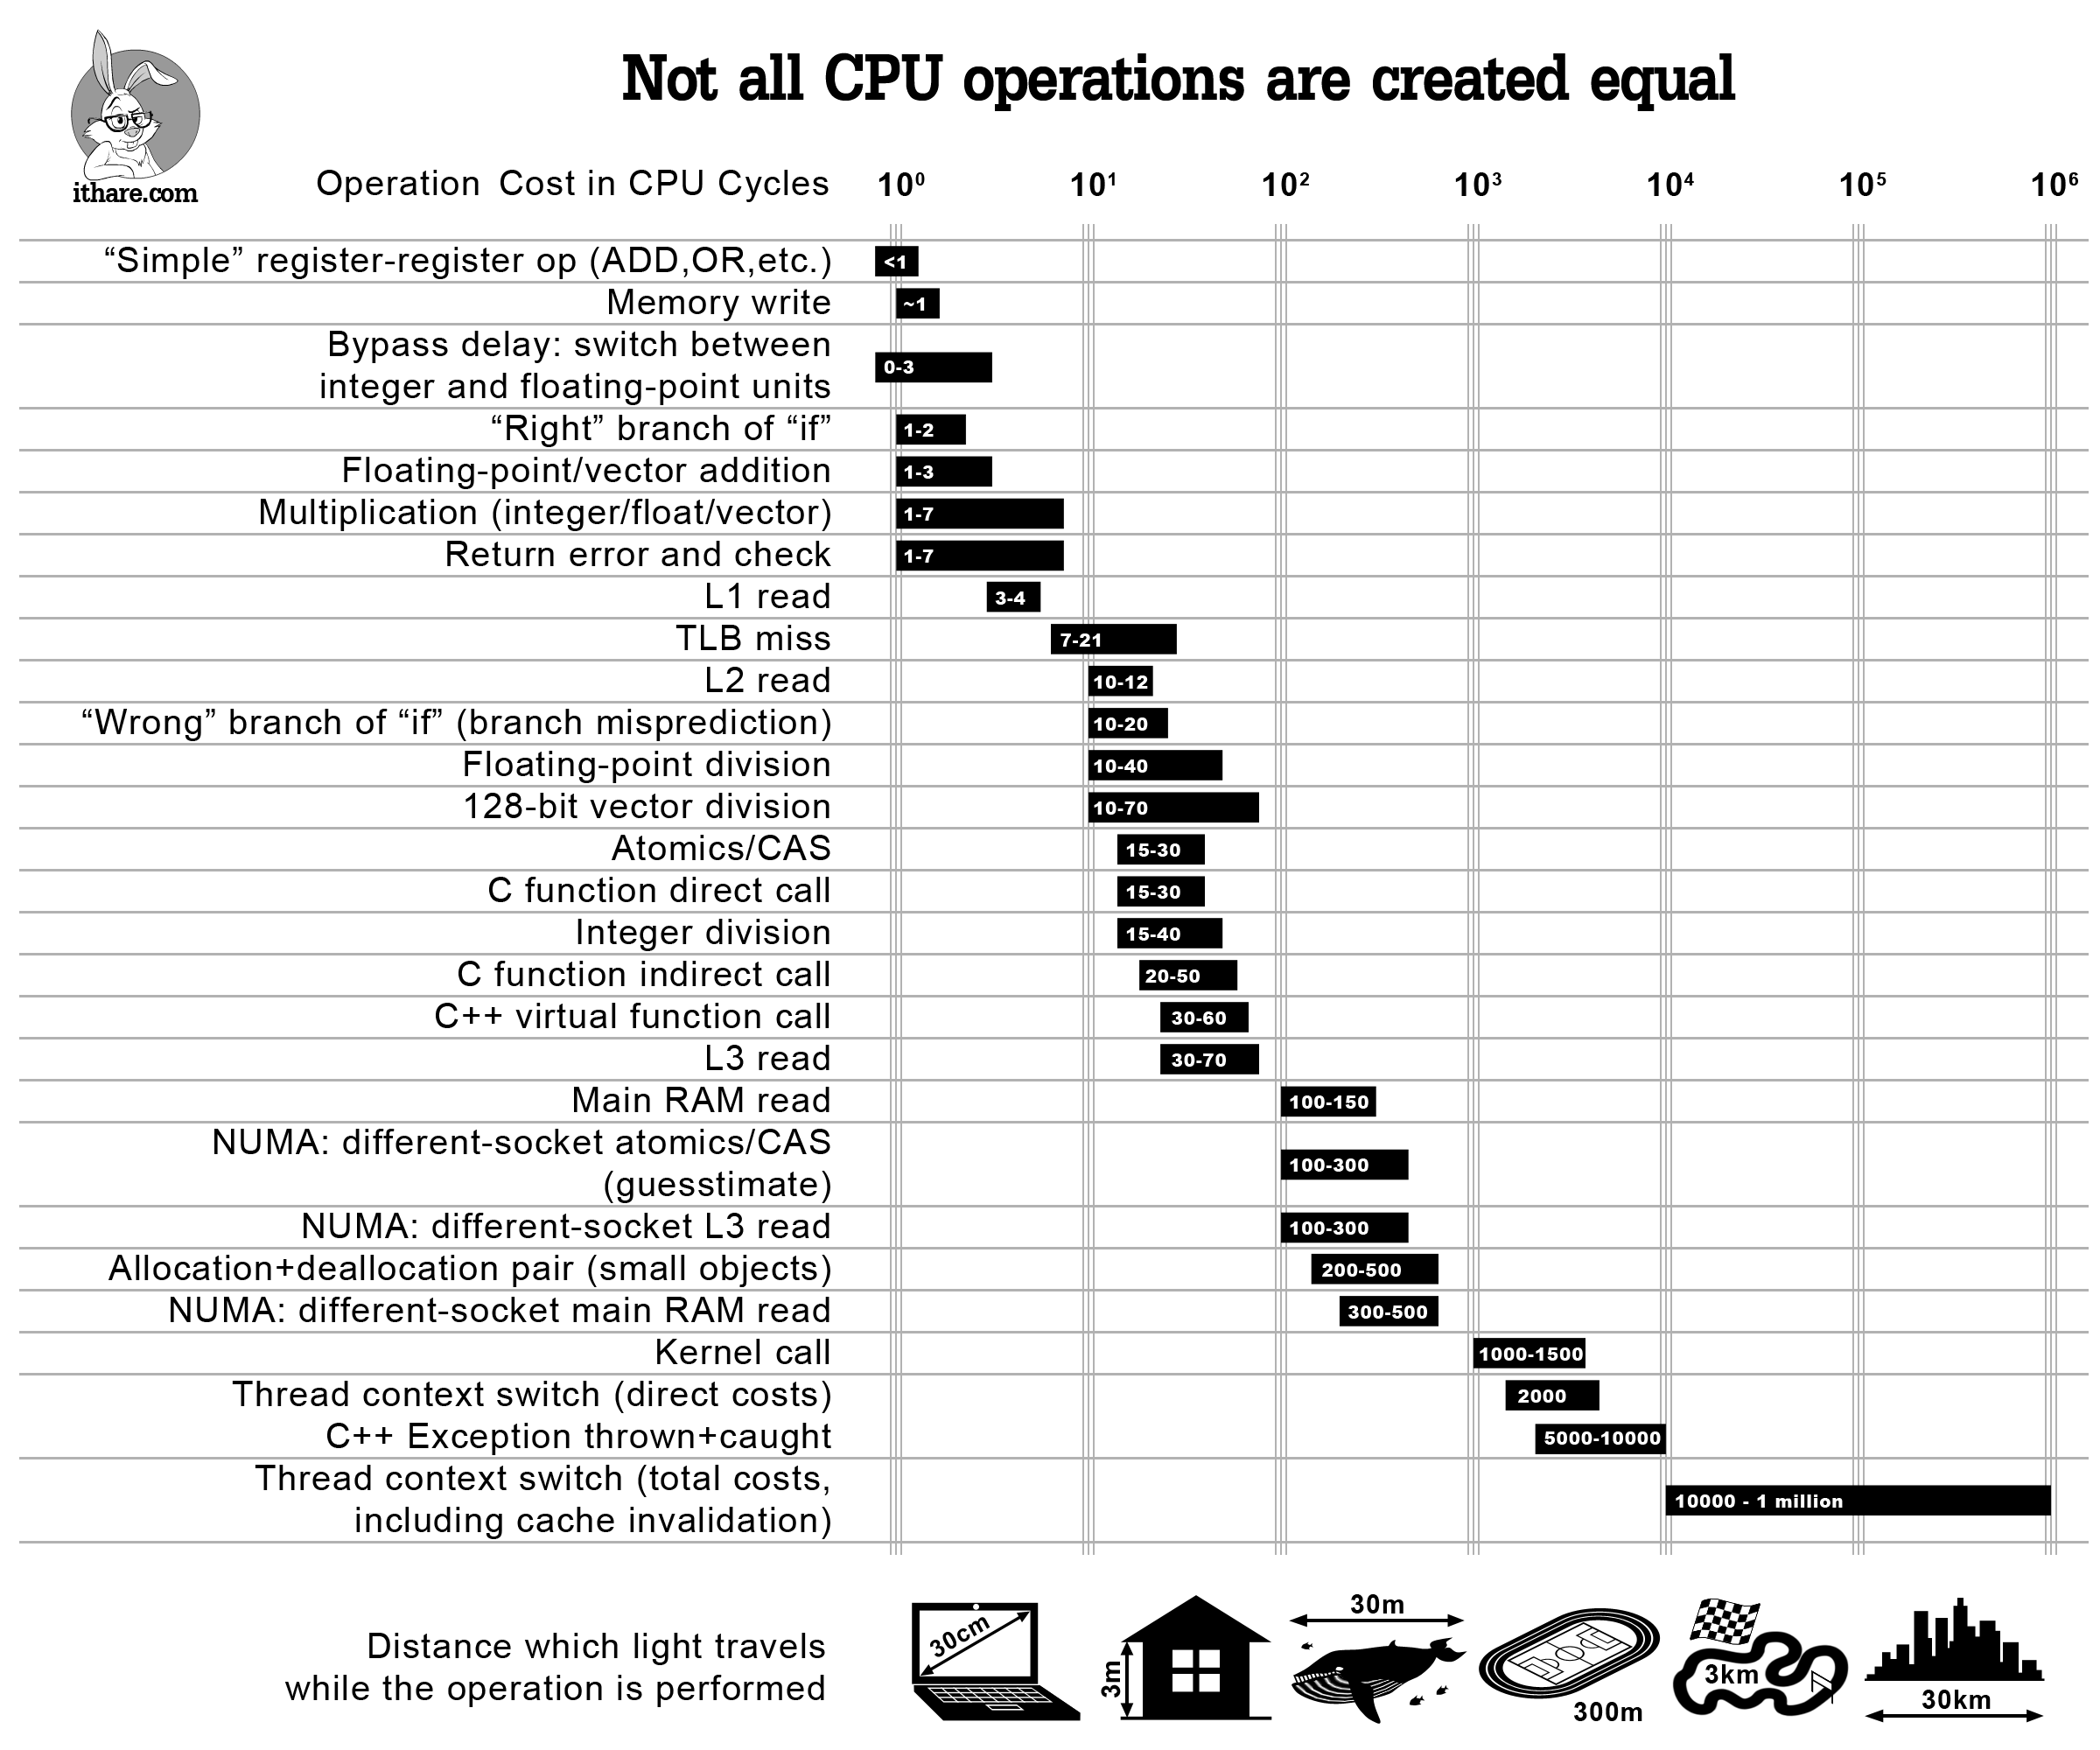
\includegraphics[width=9cm]{time}\\
   \end{center}
\end{frame}


\begin{frame}[fragile]{Modèle de mémoire en Java}
  \begin{block}{Le mot-clé \lstinline{volatile} en Java}
    \begin{itemize}
    \item Les variables \lstinline{volatile} sont linéarisables
    \item Gestion par le système
      \begin{itemize}
      \item Limite les optimisations du compilateur
      \item Limite l'utilisation des caches
      \end{itemize}
    \end{itemize}
  \end{block}
\vfill
  \begin{alertblock}{Toute variable doit être :}
    \begin{itemize}
    \item soit déclarée \lstinline{final}
    \item soit déclarée \lstinline{volatile}
    \item soit uniquement accédée séquentiellement
      \begin{itemize}
      \item exemple des variables locales
      \item par exemple en section critique
      \item lectures et écritures ordonnées par ``happened before''
      \end{itemize}
    \end{itemize}
  \end{alertblock}
\vfill
\begin{citing}
\item \href{https://docs.oracle.com/javase/specs/jls/se7/html/jls-17.html#jls-17.4}{Voir la spécification officielle de la JVM, chapitre 17.4}
\end{citing}
\end{frame}


\begin{frame}{La relation ``happened before'' (ordre causal)}
  $e\mapsto e'$ si l'une des conditions s'applique :    
  \begin{itemize}
  \item \structure{Ordre de programme :} le même thread produit $e$ puis $e'$
  \item \structure{Ordre de synchronisation :} ordre total sur un sous-ensemble d'actions
  \begin{itemize}
    \item Entrée et sortie d'un block \lstinline{synchronized} ;
    \item Lecture et écriture d'une variable \lstinline{volatile} ;
    \item Lancement d'un thread $\mapsto$ première action du thread
    \item $t.interrupt() \mapsto$ détection de l'interruption 
      \begin{itemize}
      \item \lstinline{throw InterruptedException}, \lstinline{interrupted()} ou \lstinline{isInterrupted()}
      \end{itemize}
    \item Dernière action d'un thread $\mapsto$ détection de terminaison
      \begin{itemize}
      \item $t.join()$ ou $t.isAlive()$
      \end{itemize}
    \item Écriture d'une valeur par défaut $\mapsto$ première action d'un thread
  \end{itemize}
  \item \structure{Vie d'un objet :} $e$ est la fin du constructeur et $e'$ l'appel de \lstinline{finalizer}.
  \item \structure{Transitivité :} $\exists e'', e\mapsto e'' \mapsto e'$
  \end{itemize}
  \begin{alertblock}{Happened before consistency pour une variable}
  \begin{itemize}
  \item \alert{Si les seules opérations concurrentes sont des lectures,}
  \item alors chaque lecture retourne la dernière valeur écrite
  \end{itemize}
  \end{alertblock}
\end{frame}

\begin{frame}[fragile]{Exemple (schématique) }
  \begin{tikzpicture}
    \fill<2->[alertColor!20, rounded corners] (3.1,6.85) rectangle (7.5,7.15);
    \fill<2->[alertColor!20, rounded corners] (3.55,4.85) rectangle (6.2,5.15);
    \fill<2->[alertColor!20, rounded corners] (4.5,3.2) rectangle (6.3,3.5);
    \draw (5,5) node{\begin{minipage}{5cm}\begin{lstlisting}[numbers=none]
  class Future<T> {


    final Callable<T> task;
    volatile boolean isDone = false;
    T value = null;


    void init() { // par thread du thread pool
      value = task.call();
      isDone = true;
    }


    T get() { // par autre thread
      while(!isDone);
      return value;
    }


  }
  \end{lstlisting}\end{minipage}
  };

    \draw<3->[|->, structure, thick, rounded corners] (6.5,5.2) -- (6.5,5) -- (6.2,5);
    \draw<3->[structure] (6.5,4.65) node[right] {Ordre de programme};
    \draw<2->[|->, alertColor, thick, rounded corners] (3.5,5) -- (3,5) -- (3,3.3) -- (3.5,3.3);
    \draw<2->[alertColor] (3.1,4.25) node[right]{Ordre de synchronisation};
    \draw<3->[|->, structure, thick, rounded corners] (6.3,3.35) -- (6.5,3.35) -- (6.5,3) -- (6,3);
    \draw<3->[structure] (6.15,2.7) node {Ordre de programme};
    \draw<4>[|->, exampleColor, thick, rounded corners] (7.5,5.3) -- (10,5.3) -- (10,3) -- (6.5,3);
    \draw<4>[exampleColor] (10,4.15) node[right] {Transitivité};

\end{tikzpicture}
\end{frame}

\begin{frame}[fragile]{Retour sur le calcul de $\pi$}
  \begin{tikzpicture}
    \fill[structure!20, rounded corners] (6.7,6.2) rectangle (8.5,6.5);
    \fill[alertColor!20, rounded corners] (6.9,3.2) rectangle (8.6,3.5);
    \fill[structure!20, rounded corners] (8.05,2.52) rectangle (9.8,2.82);

    \draw[|->, alertColor, thick, rounded corners] (8.7,6.35) -- (10,6.35) -- (10,3.35) -- (8.7,3.35);
    \draw[|->, structure , thick]                  (8.4,3.1) -- (8.4,2.92);
    
    \draw (5,5) node{\begin{minipage}{5cm}\begin{lstlisting}[numbers=none]
public class PiMonteCarlo implements Runnable {
  private int result = 0;
  public void run() {
    for(int i = 0; i<nbIterations; i++) {
      double x = random.nextDouble();
      double y = random.nextDouble();
      if(x*x + y*y < 1) result++;
    }
  }
  static int experiment() {
    for(int i = 0; i<nbThreads; i++) {
      tasks[i] = new PiMonteCarlo();
      threads[i] = new Thread(tasks[i]);
    }
    for(var t : threads) t.start();
    for(var t : threads) t.join();
    int result = 0;
    for(var t : tasks) result+=t.result;
    return result;
  }
}
\end{lstlisting}\end{minipage}};
  \end{tikzpicture}
\end{frame}



\begin{frame}[fragile]{Modèle de mémoire en C++}
\vfill
  \begin{block}{Le mot-clé \lstinline{volatile} en C++}
    \begin{itemize}
    \item Limite les optimisations du compilateur
    \item \alert{Ne place pas les barrières de mémoire}
    \end{itemize}
  \end{block}
\vfill
  \begin{block}{Barrières de mémoire en C++}
      \begin{itemize}
      \item \lstinline{void std::atomic_thread_fence( std::memory_order order )}
      \item Choix de synchronisation read/write, write/read...
        \begin{itemize}
        \item Seulement \lstinline{memory_order_seq_cst} chez Intel
        \end{itemize}
      \end{itemize}
  \begin{shadequote}{Phil Karlton}
    There are only two hard things in Computer Science: \\cache invalidation and naming things.
  \end{shadequote}
  \end{block}

\vspace{-3mm}
\begin{alertblock}{C++ Core Guidelines}
    \begin{description}
    \item[CP.8] \href{https://isocpp.github.io/CppCoreGuidelines/CppCoreGuidelines#Rconc-volatile}{Don’t try to use \lstinline{volatile} for synchronization}
    \end{description}
    \begin{itemize}
    \item Utiliser \lstinline{template <class T> struct std::atomic}
    \end{itemize}
  \end{alertblock}
\vspace{-1mm}
  \begin{citing}
  \item Tutoriel de Ori Lahav sur les modèles de mémoire en C++
  \end{citing}
\end{frame}


\begin{frame}[fragile]{Limite de \lstinline{volatile} : les tableaux}
  \begin{exampleblock}{Tableaux volatiles}
    \begin{lstlisting}[numbers=none]
volatile int array[];
array = new int[10];          // volatile
array[5] = 3;                 // pas volatile
    \end{lstlisting}    
  \end{exampleblock}
  \pause
  \begin{alertblock}{Première solution}
    \begin{lstlisting}[numbers=none]
class VolatileInt{public volatile int x=0;}
VolatileInt array[] = new VolatileInt[10];
array[5] = new VolatileInt(); // pas volatile
array[5].x = 3;               // volatile
    \end{lstlisting}
  \end{alertblock}
  \pause
  \begin{block}{Meilleure solution: \lstinline{java.util.concurrent.atomic.AtomicIntegerArray}}
    \begin{lstlisting}[numbers=none]
AtomicIntegerArray array = new AtomicIntegerArray(10);
array.set(5, 3);              // volatile
    \end{lstlisting}
  \end{block}    
\end{frame}


\begin{frame}[fragile]{Le compteur bloquant}
\begin{enumerate}
\item Si beaucoup de lectures :

  \begin{tikzpicture}
    \fill[alertColor!20, rounded corners] (4.3,5.7) rectangle (5.8,6);
    \draw (5,4.85) node{\begin{minipage}{5cm}\begin{lstlisting}[numbers=none]
class Counter {
  private volatile int value=0;
  public synchronized void increment() {
    ++value;
  }
  public int get() {
    return value;
  }
}
\end{lstlisting}\end{minipage}};
  \end{tikzpicture}
\item Si plus d'incrémentations que de lectures :

\begin{tikzpicture}
    \fill[alertColor!20, rounded corners] (4,4.35) rectangle (6.4,4.65);
    \draw (5,4.85) node{\begin{minipage}{5cm}\begin{lstlisting}[numbers=none]
class Counter {
  private int value=0;
  public synchronized void increment() {
    ++value;
  }
  public synchronized int get() {
    return value;
  }
}
\end{lstlisting}\end{minipage}};
  \end{tikzpicture}
\end{enumerate}
\end{frame}


\mode<all>

 
\section{Conclusion}
\subsection{Bilan}
\begin{frame}[fragile]{Bilan}

  \vfill
  \begin{block}{Calcul réparti en mémoire partagée}
    \begin{itemize}
    \item La concurrence crée de nouveaux problèmes de sûreté
    \item La synchronisation pour les résoudre limite la vivacité
    \end{itemize}
  \end{block}
  \vfill
  \begin{block}{Attention aux contre-intuitions !}
    \begin{itemize}
    \item \lstinline{x++} \alert{ne signifie pas} \og incrémenter \lstinline{x} \fg
    \item \lstinline{A ; B} \alert{ne signifie pas} \og exécuter \lstinline{A} puis \lstinline{B} \fg
    \item \og Écrire dans une variable \fg{} est une notion très floue
    \item ...
    \end{itemize}
  \end{block}
  \vfill
  \begin{alertblock}{Limiter le partage des données}
    \begin{itemize}
    \item Utiliser des objets immutables
    \item Ne pas partager si possible
    \end{itemize}
  \end{alertblock}
  \vfill
\end{frame}


\subsection{Perspectives}

\begin{frame}[fragile]{Un monde en constante évolution}

 \begin{block}{Modèles à passage de messages}
    \begin{itemize}
    \item Cloud computing
    \item Réseaux pair-à-pair
    \end{itemize}
  \end{block}

 \begin{block}{Algorithmique du réparti en calcul réparti}
    \begin{itemize}
    \item Problèmes de calculabilité
    \item Problèmes de complexité
    \end{itemize}
 \end{block}

   \begin{block}{Modèles de programmation concurrente}
    \begin{itemize}
    \item Loom project et Java 21
    \begin{itemize}
    \item Threads virtuels
    \item Concurrence structurée
    \end{itemize}
    \item Modèles de concurrence de Go, Gleam, Rust...
    \end{itemize}
  \end{block}
\end{frame}




\begin{frame}[fragile]{Mémoire transactionelle}
  \vFill
  \begin{block}{Mémoire transactionelle logicielle}
    \begin{lstlisting}
void increment (Register<Integer> X) {
  Transaction t = new STMTransaction();
  while (!t.isCommited()) {
    try {
      t.begin();
      X.write(t, X.read(t) + 1);
      t.try_to_commit();
    } catch (AbortException e) {}
  }
}
    \end{lstlisting}
  \end{block}
  \pause
  \begin{alertblock}{TP4}
    \begin{enumerate}
    \item Lire l'article sur Madoc
 
    \item Implémenter l'algorithme TL2
    \end{enumerate}
  \end{alertblock}
  \vFill
  
  \begin{citing}
  \item[IR09] Damien Imbs et Michel Raynal. \textit{Software transactional memories: an approach for multicore programming}. PaCT 2009
    \end{citing}
\end{frame}



\end{document}

\endinput
